\documentclass[11pt,a4paper]{article}
\usepackage[T1]{fontenc}
\usepackage[utf8]{inputenc}
\usepackage{lmodern}
\usepackage[margin=22mm]{geometry}
\usepackage{amsmath,amssymb,booktabs,tabularx,array}
\usepackage{enumitem,xcolor,tikz,xurl,hyperref}
\usetikzlibrary{arrows.meta,positioning,calc,fit}
\hypersetup{colorlinks=true,linkcolor=blue!55!black,urlcolor=blue!55!black,
  citecolor=blue!55!black,pdftitle={Abstract Machines: Steppers, Worlds and Semantic Connections}}
\setlength{\emergencystretch}{3em}
\setlength{\parskip}{5pt}
\setlength{\parindent}{0pt}
\setlist{nosep,leftmargin=*}
\definecolor{ink}{HTML}{18344D}
\definecolor{sea}{HTML}{087F8C}
\definecolor{amber}{HTML}{A86513}
\definecolor{pale}{HTML}{EDF5F8}
\tikzset{
  box/.style={draw=ink!65,fill=pale,rounded corners=2pt,align=center,
    text width=35mm,minimum height=13mm,inner sep=5pt,font=\small},
  wide/.style={box,text width=48mm},
  smallbox/.style={box,text width=27mm},
  future/.style={box,draw=amber,dashed,fill=amber!5},
  arr/.style={-{Stealth[length=2mm]},thick,draw=ink},
  hint/.style={font=\scriptsize,align=center,text=ink},
  boundary/.style={draw=amber,dashed,rounded corners,inner sep=7pt}
}
\newcommand{\code}[1]{\texttt{\detokenize{#1}}}
\newcommand{\name}[1]{\textup{\Urlmuskip=0mu\relax\nolinkurl{#1}}}
\newcommand{\sources}[1]{\par\smallskip{\small\raggedright\textbf{Existing owners.} #1\par}}
\newcommand{\scope}[1]{\par\smallskip\begin{quote}\small\textbf{Boundary.} #1\end{quote}}
\newcommand{\diagramcaption}[1]{\par{\small\color{ink}#1\par}\medskip}
\newcommand{\run}{\mathsf{run}}
\newcommand{\resume}{\mathsf{resume}}
\newcommand{\obs}{\mathsf{obs}}

\title{\color{ink}Abstract Machines\\[3pt]
  \large Steppers, retained worlds and semantic connections in Mettapedia}
\author{Mettapedia Working Notes}
\date{16 October 2026}

\begin{document}
\maketitle
\begin{abstract}
An abstract machine records unfinished work, its environment or world, and
what has become observable. This overview connects the functional,
categorical, call-by-need, refocusing, GSLT, rho, C and proof machines through their
steppers, observers and resumption laws. Scoped, licensed composition supplies
a common checking interface; costed relational stages and functional path
transport supply two constructed categorical organizations of machines. The common execution contracts
preserve distinct evaluation strategies and logical theories. Deterministic
regions, probabilistic execution, zippers and typed graph holes supply
ingredients of a candidate computational-metagraph machine. Diagrams
distinguish constructed connections from remaining obligations.
\end{abstract}

\section{One map, several machines}

The language rules say what a computation means. The machine says how its
unfinished work is represented. A VM additionally supplies a code image,
loader and instruction-admission contract. A native implementation must
realize those representations and transitions under its memory and service
assumptions. Each connection needs its own theorem or qualification evidence.
Section~\ref{sec:checking} develops the corresponding proof-checking machine:
what follows from what, under which conditions, and how its evidence composes.

\begin{center}
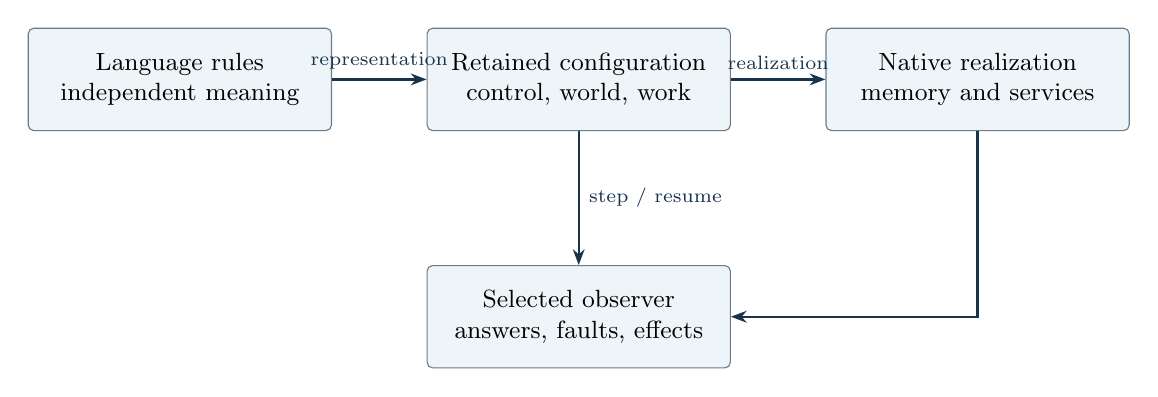
\begin{tikzpicture}
  \node[box] (source) {Language rules\\independent meaning};
  \node[box,right=12mm of source] (machine) {Retained configuration\\control, world, work};
  \node[box,right=12mm of machine] (native) {Native realization\\memory and services};
  \node[box,below=17mm of machine] (observer) {Selected observer\\answers, faults, effects};
  \draw[arr] (source) -- node[hint,above]{representation} (machine);
  \draw[arr] (machine) -- node[hint,above]{realization} (native);
  \draw[arr] (machine) -- node[hint,right]{step / resume} (observer);
  \draw[arr] (native.south) |- (observer.east);
\end{tikzpicture}
\end{center}
\diagramcaption{Similar outputs on examples test a connection. They do not replace a
general correspondence theorem between independently defined semantics.}

\begin{tabularx}{\linewidth}{@{}lX@{}}
\toprule
Family & Distinguishing retained information \\
\midrule
CEK / Krivine & Value environments and argument frames / unevaluated closures. \\
Categorical CAM & Register, compiled closures, remaining code and value stack. \\
Branch-local Need & Cell origins, memo states, branch worlds and reuse identity. \\
Refocusing & Legal context stack, focused redex and ordered candidate attempts. \\
GSLT / rho & Scoped search jobs, unmet obligations and occurrence-bearing receipts. \\
C-language core & Byte memory, continuations, pending expression occurrences. \\
\bottomrule
\end{tabularx}

The historical \emph{Categorical Abstract Machine} and the machine for the
\emph{C language} are different instances. Neither supplies a universal fastest
strategy. The broader observer and logical-world foundation is developed in
\name{papers/metatheory.tex}.

\newpage
\section{What the common stepper must retain}

An individual run records an execution sequence; MeTTa need not promise one
global answer enumeration order. Cross-machine observations may retain the
multiset of full answer occurrences, including multiplicity, bindings and
provenance, while forgetting enumeration. Stronger ordered theorems qualify a
selected worker policy. Within each worker, resumption keeps its captured
publication and remaining work without replay or omission. Bounded selection
can choose different valid occurrences under different strategies. Observable
effects and causal dependencies require their own preservation laws.

The simplest core is a state type, a loader and a partial step function.
A missing step alone does not tell us whether a program answered or got stuck.
The productive event interface therefore makes successful completion explicit:
\[
 \mathsf{step}:S\longrightarrow
 \mathsf{Option}\bigl(\mathsf{Transition}(S,E,V,Q)\bigr).
\]
Here $E$ is an event, $V$ a verdict and $Q$ a request. A transition can perform
silent administration, publish events, finish, fail with events, or call out
while saving its continuation. An absent transition is reported as stuck.

\begin{center}
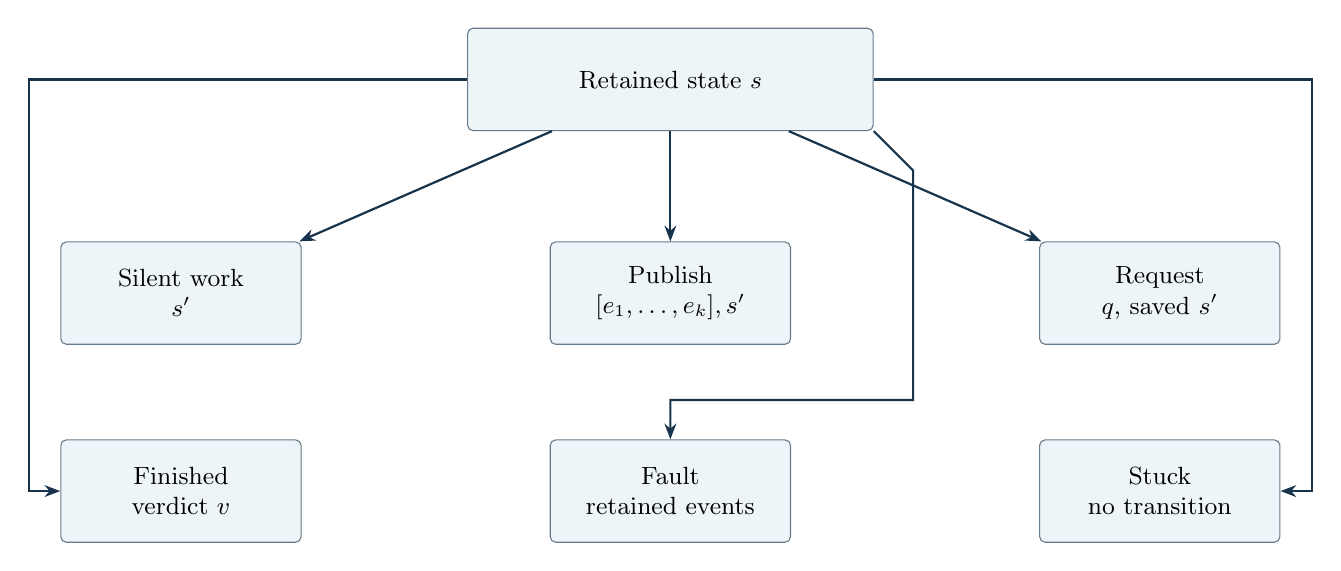
\begin{tikzpicture}
  \node[wide] (s) {Retained state $s$};
  \node[smallbox,below left=14mm and 21mm of s] (silent) {Silent work\\$s'$};
  \node[smallbox,below=14mm of s] (publish) {Publish\\$[e_1,\ldots,e_k],s'$};
  \node[smallbox,below right=14mm and 21mm of s] (call) {Request\\$q$, saved $s'$};
  \node[smallbox,below=12mm of silent] (final) {Finished\\verdict $v$};
  \node[smallbox,below=12mm of publish] (fault) {Fault\\retained events};
  \node[smallbox,below=12mm of call] (stuck) {Stuck\\no transition};
  \draw[arr] (s) -- (silent); \draw[arr] (s) -- (publish); \draw[arr] (s) -- (call);
  \draw[arr] (s.west) -- ++(-3mm,0) -| ([xshift=-4mm]final.west) -- (final.west);
  \draw[arr] (s.east) -- ++(3mm,0) -| ([xshift=4mm]stuck.east) -- (stuck.east);
  \draw[arr] (s.south east) -- ++(5mm,-5mm)
    |- ([yshift=5mm]fault.north) -- (fault.north);
\end{tikzpicture}
\end{center}
\diagramcaption{The arrows show possible transition or outcome kinds, not a sequence
that visits every box. Exhausting fuel retains a residual; it proves neither
completion nor divergence.}

A finite runner returns an ordered event list and an outcome. After fuel
exhaustion, running longer uses the saved residual and appends only the newly
produced events. A suspended request instead needs explicit response delivery;
extra fuel does not supply its answer. Finishing,
faults, suspension, stuckness and exhaustion remain distinct. Separate price
functions account for instructions, allocations or other declared resources.
An administrative rank excludes an infinite silent stretch when its hypotheses
hold; it does not assume the whole program terminates.

\subsection*{Three different choices in a stepper}

Semantic alternatives, redex selection within a branch, and scheduling between
branches have different contracts. For a pure snapshot, expanding one branch
$b$ can replace its frontier occurrence by the complete bag of its successors:
\[
  F'=(F-\{b\})+\mathsf{Succ}(b).
\]
Choosing which $b$ to expand need not discard any semantic alternative. Choosing
one successor and forgetting the others changes the computation. Occurrences
remain distinct even when their printed terms agree. Fairness is a separate
obligation for an infinite search; a finite pause establishes no exhaustive
answer collection.

Redex selection inside a branch must still follow its evaluation policy.
Call-time choice illustrates why unrestricted term rewriting is insufficient:
copies of one shared choice must not become independent choices. Let-rewriting
provides an explicit reduction presentation with soundness and completeness
against its call-time-choice semantics~\cite{LetRewriting}. Our branch-local
Need instance has its own independently stated judgments and adequacy laws;
that precedent does not establish native MeTTa adequacy automatically.

A source-level step also need not be one implementation instruction.
Clements, Flatt and Felleisen separately prove preservation by instrumentation
and reconstruction of the source reduction sequence~\cite{AlgebraicStepper}.
The corresponding obligation here is a constructed source/configuration map
and a productive block simulation. A debugger may expose that semantic view
without making all optimizer frames ordinary program observations.

Scheduling shared effects requires further evidence: commuting actions,
isolation, or an explicit serialization policy. The answer observer must also
be declared. Alpha-renaming of internal bindings cannot erase a string that
an ordinary operation has already produced from a variable's displayed name.
These distinctions prevent a scheduler-independence claim from silently
changing sharing, effects, or the language's observations.

\subsection*{The strongest useful form of correspondence}
A related source/native pair should reproduce the same selected occurrences,
with related residuals, at every relevant observation boundary. Native
administration may take several steps for one source step. A ranked block
simulation licenses that difference without erasing observable failures.
The backward direction establishes no invention; the forward direction
establishes that source behavior is realized. Cost bounds need an explicit
resource model in addition to behavioral correspondence.

\subsection*{A logical machine with replaceable backends}

The stable MeTTa machine is specified at the level of scoped evaluation
operations. Its configuration retains the term or task, binding constraints,
continuation, answer occurrences, observable world and required authority.
The selected language profile determines argument evaluation, rule freshening,
choice sharing, returned-value treatment and effects. A frame's address,
hash-table layout or symbol number belongs to a backend realization.
Logical object identity, freshness and ownership remain obligations wherever
the declared operations can observe them; changing addresses does not license
merging identities.

The representation boundary is a relation $R(b,s)$ between a backend state
$b$ and a logical configuration $s$. Several backend states may represent the
same configuration. At the declared observation boundaries, a logical step
$s\xrightarrow{e}s'$ must be realized by a finite backend block
$b\overset{e}{\Longrightarrow}b'$ with $R(b',s')$, and backend behavior must satisfy the
applicable reflection law. The block may contain internal administration;
productivity and endpoint laws prevent that administration from concealing
divergence, stuckness or faults. This is a behavioral obligation. A uniform
bound on the number or physical cost of backend instructions requires a
separate argument.

The existing event-machine interface now proves this finite-block connection
without a uniform cost premise. \name{Machine.run_related_of_one} derives
whole-prefix correspondence from local implementations of individual
inspections. Its resumption corollary retains the matched checkpoint and
appends only the suffix. Local implementations in both directions give equal
completed observations. Their outcomes retain faults, stuckness, requests and
related saved states; a separate corollary reflects unbounded execution within
the current interaction region. The local contracts compose through the
actual middle state. Costed stages retain their stronger resource law.

A checked control makes the difference concrete: each logical publication
has size-dependent internal work, with no single instruction bound for all
admitted states. Both directions preserve its duplicate publications and
completed observations; resumption appends the saved suffix, while restarting
repeats the prefix. Existing forward-only controls still demonstrate that
preservation alone cannot establish completion reflection. These generic laws
do not supply the missing local CeTTa, Rust or SWI implementation instances.

The local obligations concern loading, scoped query and binding operations,
invocation and return, host effects, retained control and observation.
Their constructed laws are inputs to the existing run-composition theorems.
Assuming the complete run correspondence as an implementation field would
not discharge those obligations. A new storage representation can replace
one backend instance while the language judgments and logical machine remain
unchanged. Representation differences can be hidden only when the declared
operations and future continuations respect the proposed relation; this
includes the identities correlating several uses of one unresolved variable.

Implementation evidence has its own scope. A formal proof about a memory
model, a source-fragment correspondence under ABI and service assumptions,
and an executable conformance test support different claims. In particular,
a model theorem conditional on a backend contract is not an unconditional
correctness theorem for the compiled evaluator. Physical helper proofs
strengthen an instance; they do not become definitions of MeTTa evaluation.
The independent fixed C-core development remains a separate substantial
instance of the common theory.

The same comparison framework also guides machine redesign. Explicit
continuations can replace hidden evaluator calls; one invocation dispatcher
can replace duplicated classification; a retained binding representation can
replace repeated reconstruction. These are machine refinements when the
specified observations are preserved. They earn efficiency claims only through
an appropriate cost comparison and measurements of the actual implementation.
A small change to the evaluation policy may instead yield a more coherent
language. Such a change is an explicitly compared semantic candidate, with
programs distinguishing the two policies and laws explaining the gain. It is
not evidence for equivalence under the old observation. The relevant choices
include fault versus ordinary failure, repeated evaluation versus ready values,
and who may inspect, advance or publish a retained computation. A licensed
transition and possession of authority to perform it remain separate judgments.
Execution determinism, answer cardinality and probabilistic meaning are
separate dimensions (Section~\ref{sec:contracts}). Focused graph holes and
changes of resolution follow in Sections~\ref{sec:holes} and~\ref{sec:zoom}.

\sources{\name{Mettapedia/Machines/MachineSubstrate.lean},
\name{Mettapedia/Machines/ProductiveCoreAdapters.lean},
\name{Mettapedia/GSLT/Distinction/ProductiveBlocks.lean},
\name{Mettapedia/GSLT/Distinction/SpanTransport.lean},
\name{Mettapedia/GSLT/Distinction/SimulationComposition.lean},
\name{Mettapedia/GSLT/Distinction/OrderedAdministration.lean}.}
\scope{These are common execution interfaces. They do not make the selected
logical kernels equal, or automatically prove a native evaluator refines them.}

\newpage
\section{CEK and Krivine: one syntax, different demands}

Both examples use de Bruijn lambda terms with natural-number literals.
The CEK-shaped machine implements left-to-right call by value. Its environment
contains values; its continuation first remembers an argument, then the
evaluated function. The Krivine-shaped machine uses call by name: its argument
stack contains closures whose evaluation is deferred.

\subsection*{CEK stepper}
For an application, evaluate the operator, evaluate the argument, and enter the
function's captured environment extended by the argument value.
\begin{center}
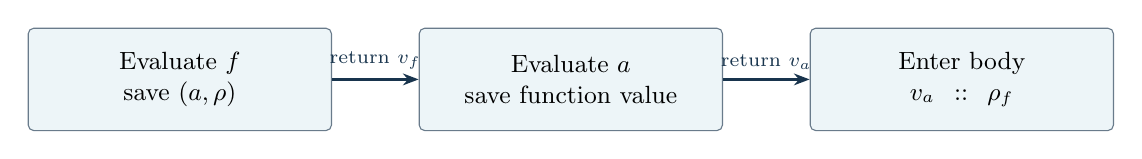
\begin{tikzpicture}
  \node[box] (f) {Evaluate $f$\\save $(a,\rho)$};
  \node[box,right=11mm of f] (a) {Evaluate $a$\\save function value};
  \node[box,right=11mm of a] (body) {Enter body\\$v_a::\rho_f$};
  \draw[arr] (f) -- node[hint,above]{return $v_f$} (a);
  \draw[arr] (a) -- node[hint,above]{return $v_a$} (body);
\end{tikzpicture}
\end{center}
\subsection*{Krivine stepper}
Push the argument closure, enter the operator, and bind the saved closure when
a lambda is reached. A variable lookup resumes its closure.
\begin{center}
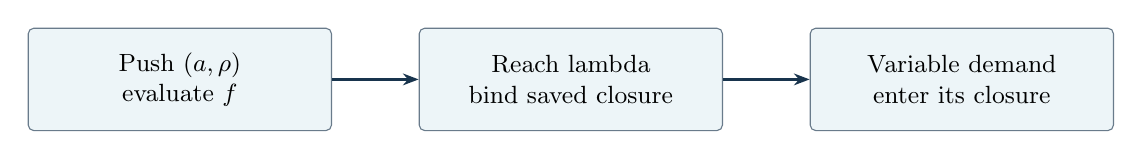
\begin{tikzpicture}
  \node[box] (save) {Push $(a,\rho)$\\evaluate $f$};
  \node[box,right=11mm of save] (lam) {Reach lambda\\bind saved closure};
  \node[box,right=11mm of lam] (use) {Variable demand\\enter its closure};
  \draw[arr] (save) -- (lam); \draw[arr] (lam) -- (use);
\end{tikzpicture}
\end{center}

The existing \name{CEK.eval_to_machine} and
\name{Krivine.eval_to_machine} theorems construct machine paths from successful
independent evaluator results, uniformly in the surrounding continuation.
The common adapters expose checked answer boundaries, finite traces, resumption
and computational accounts. This endpoint development does not mechanize the
entire CPS/defunctionalization derivation.

A discriminating term is $(\lambda x.\lambda y.x)\;7\;\Omega$.
Call by value evaluates the discarded divergent argument, so its evaluator
returns no answer at every finite fuel. Call by name reaches $7$ without
demanding that argument. This is a proved strategy difference, not an
implementation defect.

\sources{\name{Mettapedia/Machines/FunctionalCorrespondence.lean},
\name{Mettapedia/Machines/MachineSubstrate.lean},
\name{Mettapedia/Machines/ProductiveFunctionalMachines.lean}.}
\scope{Call by name does not memoize. Repeated demand may repeat work;
branch-local call by need requires the additional cell and cache laws below.}

\newpage
\section{The historical Categorical Abstract Machine}

The CAM follows Cousineau--Curien--Mauny's source strategy and instruction
tables~\cite{CAM}. One indexed source grammar contains variables, lambda,
application, pairs and projections, with literals and Boolean conditionals
enabled by its extension index. Source closures retain source bodies;
machine closures retain compiled instruction lists.

\begin{center}
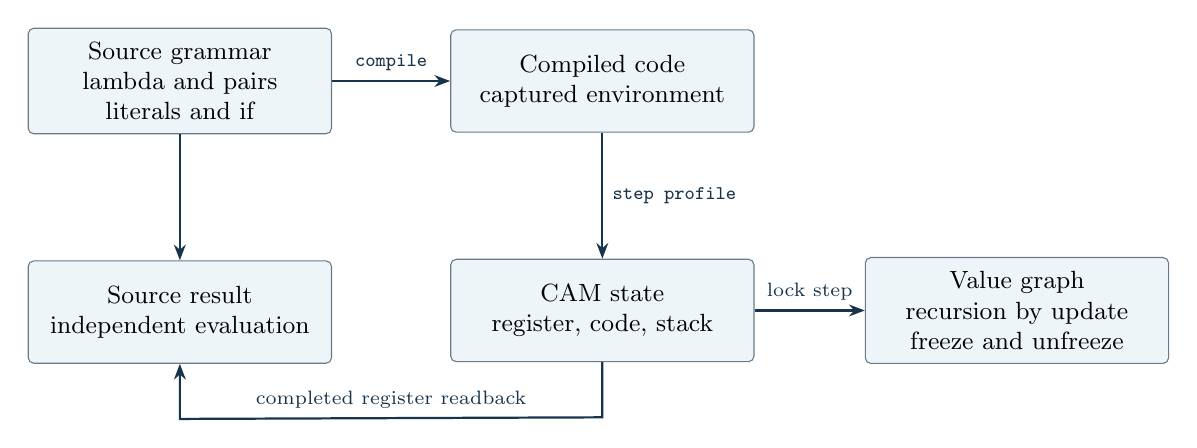
\begin{tikzpicture}
  \node[box] (source) {Source grammar\\lambda and pairs\\literals and if};
  \node[box,right=15mm of source] (code) {Compiled code\\captured environment};
  \node[box,below=16mm of source] (result) {Source result\\independent evaluation};
  \node[box,below=16mm of code] (state) {CAM state\\register, code, stack};
  \draw[arr] (source) -- node[hint,above]{\texttt{compile}} (code);
  \draw[arr] (source) -- (result);
  \draw[arr] (code) -- node[hint,right]{\texttt{step profile}} (state);
  \coordinate (sread) at ([yshift=-7mm]state.south);
  \coordinate (rread) at ([yshift=-7mm]result.south);
  \draw[arr] (state.south) -- (sread) --
    node[hint,above]{completed register readback} (rread) -- (result.south);
  \node[box,right=14mm of state] (graph) {Value graph\\recursion by update\\freeze and unfreeze};
  \draw[arr] (state) -- node[hint,above]{lock step} (graph);
\end{tikzpicture}
\end{center}
\diagramcaption{The tree machine and the value-graph machine share one instruction table.
On the tree machine's instructions they move in lock step; recursion and delay run
only on the graph.}

Application compiles to saving the environment, evaluating the operator,
restoring the environment, evaluating the argument, constructing their pair,
and applying. The actual state retains the register, remaining instructions and
stack throughout this work. The executable \name{step} agrees in both
directions with the independent \name{Transition} rules.

The shared compiler and code/value decoder have proved inverses on their
admitted images, including captured closure environments.
\name{evaluation_iff_execution} connects independent evaluation to completed
neutral-profile execution at both indices; completion requires empty code
and stack. A conditional evaluates its condition, restores the saved environment
and runs only the selected arm. A non-Boolean condition can be stuck.
\name{Lambda.proposition_3_2} connects historical scoped weak source reduction
to execution and readback at either syntax index, including literal and
conditional source terms and captured scoped environments. The strategy does
not reduce under a lambda.
Typed source formation constructs actual Cartesian closed morphisms;
\name{Typed.evaluation_iff_strict_execution} and the meaning theorems connect
the active instruction table to that interpretation.

The historical constant-free compiler remains the disabled-index specialization;
its no-quotation/no-branch laws and typed Cartesian-closed results keep that
scope. The enabled source uses the existing native quotation/branch instructions.

Recursion and delayed evaluation follow the paper's Sections~4 and~5 on a value
graph. Heap cells are couples, closures and frozen computations. Allocation
appends a cell; \name{wind} updates the second component of an existing couple,
as LISP's \name{rplacd} does. Recursion compiles as in the paper's Table~6 and
leaves the cyclic closure $c = C{:}(s,c)$ in the register. \name{freeze} builds a
frozen computation and \name{unfreeze} forces it at strict positions (Table~7);
forcing is by name. The module records two corrections to the published listing:
\name{unfa} and \name{unfb} rebuild the couple with exchanged components, and the
\name{letrec} code of Section~5 has a stray \name{swap}.

An independent big-step judgment covers recursion, frozen values and strict
primitives. \name{evaluation_iff_execution} relates it to completed execution
without assuming termination; executions keep the caller's code and stack and never
change existing cells. Heap words represent source values by finite derivations.
A cycle represents both a recursive value and its unfolding
(\name{Represents.not_functional}), so source syntax is not observable on the graph;
represented words agree with the depth-indexed unfoldings of their values, and
bisimilarity is agreement at every depth (\name{Represents.bisimilar_iff}).
\name{refinement} and \name{abstraction} are cost-one simulations between the tree
machine and the graph machine on the tree's instructions. Allocation keeps the heap
topologically ordered; \name{wind} breaks the order, and its cycle has no tree
unfolding (\name{windHeap_no_unfolding}). Controls run the paper's factorial and
lazy stream, a divergent loop, and stuck cases.

A memoizing variant uses the existing branch-local demand store. Each frozen
cell has its own allocation identity and immutable origin. Starting evaluation
records an owner; nested update frames retain the caller until the result can
be committed. Later forces read the completed cache without restarting its
producer. Separate allocations of equal source terms remain separate demands.

The independent source judgments \name{Need.Evaluation},
\name{Need.Invocation} and \name{Need.Force} use source constructors, an arena
and a demand store. They have no machine control or transition premise.
\name{Need.evaluation_iff_execution} proves both directions for complete values
and the entire retained world, including recursion, conditionals, cached hits
and nested updates. Its source-arena condition requires stored closure and
suspension bodies to be compiled source terms; the empty loader establishes
that condition directly. Active ownership blocks recursive demand. This is
explicit memoizing semantics, distinct from the historical by-name strategy.

\sources{\name{Mettapedia/Machines/CategoricalAbstractMachine.lean},
\name{Mettapedia/Machines/CategoricalAbstractMachineGraph.lean},
\name{Mettapedia/Machines/CategoricalAbstractMachineControls.lean}.}
\scope{Cartesian closure supplies typed meaning, not recursion or update; the graph
machine gives those their own operational laws. The extended readback and
memoizing correspondence are constructed. Logical instruction counts do not
by themselves establish physical performance or a native-code compiler.}

\newpage
\section{Branch-local Need: choose once, reuse in that branch}

The existing call-time-choice core separates value expressions from
computations. The distinction follows the call-time-choice separation between
shared demand and unrestricted rewriting~\cite{LetRewriting}. Its runtime
distinguishes a memoized implicit suspension,
a resampled implicit thunk, and explicitly quoted code. A cell retains its
original code and environment while its cache changes state.

\begin{center}
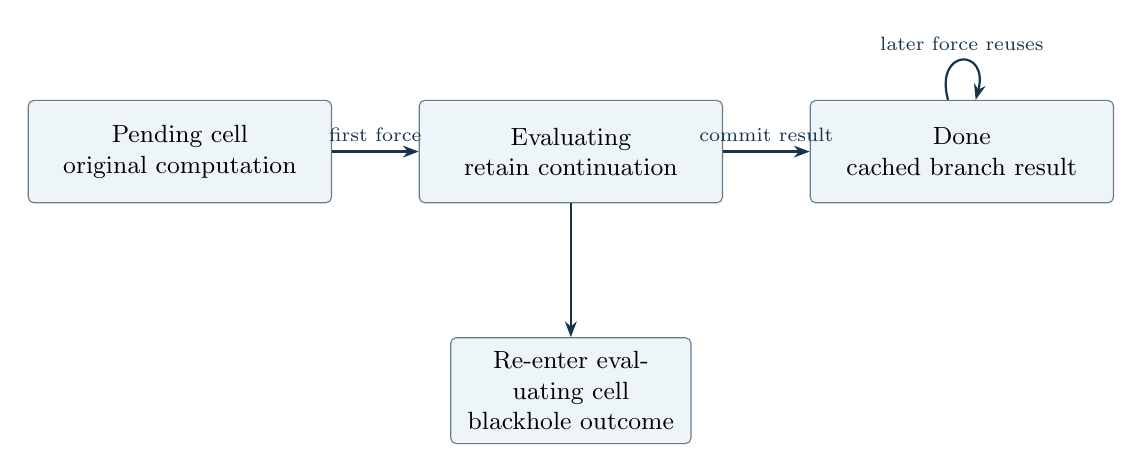
\begin{tikzpicture}
  \node[box] (pending) {Pending cell\\original computation};
  \node[box,right=11mm of pending] (running) {Evaluating\\retain continuation};
  \node[box,right=11mm of running] (done) {Done\\cached branch result};
  \draw[arr] (pending) -- node[hint,above]{first force} (running);
  \draw[arr] (running) -- node[hint,above]{commit result} (done);
  \draw[arr] (done) to[loop above,looseness=5]
    node[hint,above]{later force reuses} (done);
  \node[smallbox,below=17mm of running] (cycle) {Re-enter evaluating cell\\blackhole outcome};
  \draw[arr] (running) -- (cycle);
\end{tikzpicture}
\end{center}

\begin{center}
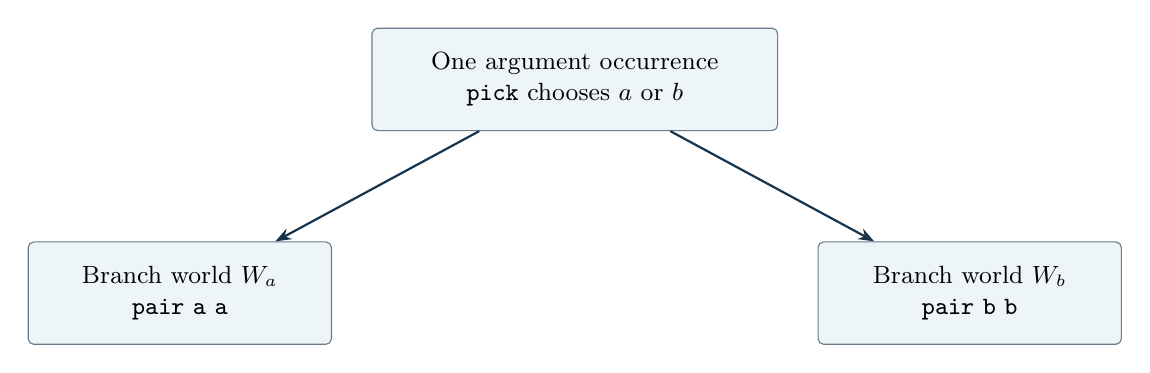
\begin{tikzpicture}
  \node[wide] (pick) {One argument occurrence\\\texttt{pick} chooses $a$ or $b$};
  \node[box,below left=14mm and 5mm of pick] (a) {Branch world $W_a$\\\texttt{pair a a}};
  \node[box,below right=14mm and 5mm of pick] (b) {Branch world $W_b$\\\texttt{pair b b}};
  \draw[arr] (pick) -- (a); \draw[arr] (pick) -- (b);
\end{tikzpicture}
\end{center}
\diagramcaption{Both uses share one chosen value in their own branch. A cache written
in $W_a$ does not become the cache of $W_b$. Separate argument occurrences can
still make independent choices.}

The natural semantics \name{Derives} is independently defined. The
\name{adequacy} and \name{observes_iff_halts} results connect it to the
unchanged branch-local Need machine in both directions, keeping the ordered
list of outcomes and duplicate occurrences. Failure and blackhole outcomes
are explicit. The strict-position theorem ensures primitives receive normal
forms under the modeled binding policies.

Quoted code is a value until explicit activation. Structural observation may
materialize an implicit pending cell under its original world and force rights;
it must not infer execution permission from a callable-looking written subtree.

\sources{\name{Mettapedia/Machines/BranchLocalNeed/CallTimeChoiceSpec.lean},
\name{Mettapedia/Machines/BranchLocalNeed/CallTimeChoiceBackward.lean},
\name{Mettapedia/Machines/BranchLocalNeed/CallTimeChoiceStrict.lean},
\name{Mettapedia/Machines/BranchLocalNeed/SharedContinuationInstance.lean}.}
\scope{This is source/model adequacy. Full native heap, producer/world identity,
resource retention and evaluator correspondence require their own joins.}

\newpage
\section{Refocusing: retain the route to the next redex}

A reduction evaluator repeatedly decomposes a term, contracts a redex, and
plugs the result back into its context. Refocusing keeps the context and searches
from the contractum, avoiding unnecessary reconstruction when the strategy's
laws justify it~\cite{Refocusing}.

\begin{center}
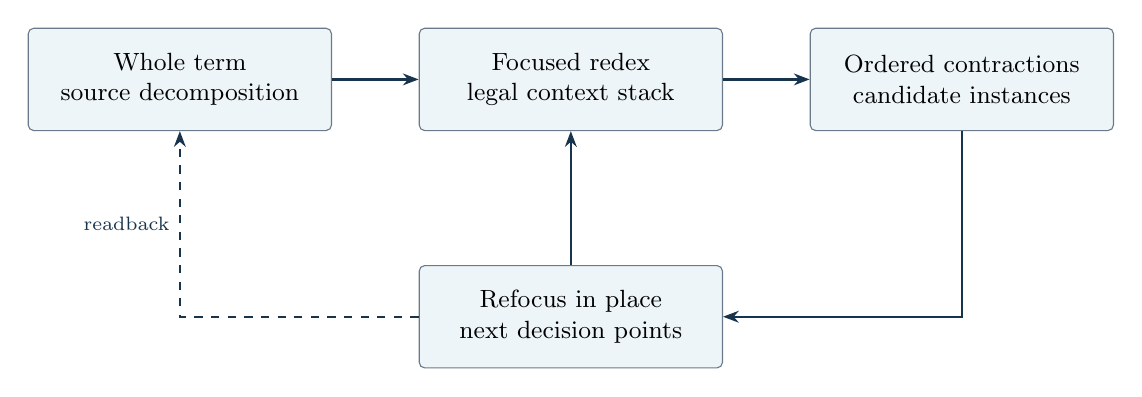
\begin{tikzpicture}
  \node[box] (whole) {Whole term\\source decomposition};
  \node[box,right=11mm of whole] (focus) {Focused redex\\legal context stack};
  \node[box,right=11mm of focus] (contract) {Ordered contractions\\candidate instances};
  \node[box,below=17mm of focus] (refocus) {Refocus in place\\next decision points};
  \draw[arr] (whole) -- (focus); \draw[arr] (focus) -- (contract);
  \draw[arr] (contract.south) |- (refocus.east);
  \draw[arr] (refocus) -- (focus);
  \draw[arr,dashed] (refocus.west) -| node[hint,near end,left]{readback} (whole.south);
\end{tikzpicture}
\end{center}

Frames are supplied by the evaluation strategy; their kinded stacks reuse
\name{Quiver.Path}. A structural syntax position alone does not authorize
evaluation. Traversal supplies local inspection and frame-resumption equations.
The branching strategy supplies candidates in order and ordered instantiations
for each candidate.

Inspection and rejected candidate attempts are administrative work, ranked by
\name{SearchCredits}. A focused computational step remains visible even if
its source and target terms are equal. A rejected candidate can be an empty
block; an observable fault or unmatched redex cannot be discarded on that basis.

\name{refocusingComplete} constructs reverse tracing from local
unique-decomposition laws. \name{blockSimulation}, \name{frontiers} and
\name{outcomes} preserve ordered alternatives, multiplicity and pending work.
\name{observable_stable} and \name{erasure_licensed} record the fault boundary.
\name{Authored.ruleScan_simulation} supplies an actual GSLT rule-scan instance.

\subsection*{Where generalization is still needed}
Several legal redex positions require an explicit position-selection policy.
The present unique-decomposition instance must not be silently treated as a
theorem about every parallel or nondeterministic traversal. Effectful attempts
also need a history model: erasing a rejected attempt is licensed only if its
observable commitments are accounted for.

\sources{\name{Mettapedia/Machines/Refocusing.lean},
\name{Mettapedia/Machines/RefocusingControls.lean},
\name{Mettapedia/OSLF/MeTTaIL/DerivedContexts.lean}.}
\scope{The authored rule scan is a real anchor. It does not yet establish the
full native evaluator's contextual traversal or administrative rank.}

\newpage
\section{HE and Prime: the retained representation boundary}

HE, PeTTa and declared Prime profiles are distinct language selections. A
common machine substrate can retain the selected package and its own state
without making those dialects interchangeable. Changing the selected
interpretation requires a justified crossing, not merely a new label.

The implementation boundary matters. LeaTTa is an auxiliary interpreter;
its correctness and conformance to HE are not acceptance conditions for
the CeTTa machine correspondence. A theorem about LeaTTa's instruction
worker establishes a property of that worker, even when its source judgment
is independently specified. It supplies no CeTTa transition map by itself.
HE claims must be checked against the independent judgments, the published
semantics and Rust HE; any disagreement remains explicit. The native target
is CeTTa's retained driver with its actual instruction phases, saved child
stacks, binding environments and delivery state.

\begin{center}
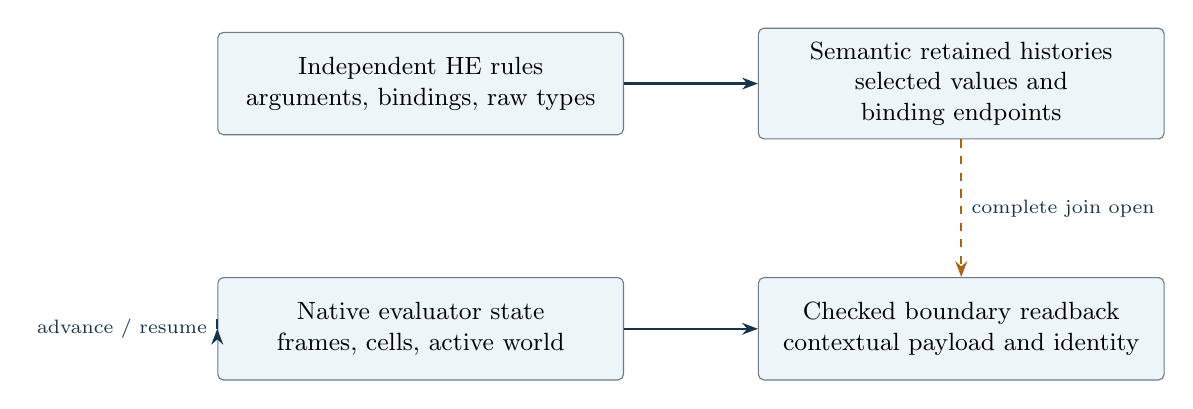
\begin{tikzpicture}
  \node[wide] (source) {Independent HE rules\\arguments, bindings, raw types};
  \node[wide,right=17mm of source] (history) {Semantic retained histories\\selected values and binding endpoints};
  \node[wide,below=18mm of source] (native) {Native evaluator state\\frames, cells, active world};
  \node[wide,right=17mm of native] (payload) {Checked boundary readback\\contextual payload and identity};
  \draw[arr] (source) -- (history);
  \draw[arr] (native) -- (payload);
  \draw[arr,dashed,draw=amber] (history) -- node[hint,right]{complete join open} (payload);
  \draw[arr] (native.west) to[out=180,in=180,looseness=3]
    node[hint,left]{advance / resume} (native.west);
\end{tikzpicture}
\end{center}

The independent argument judgment constructs an ordered history of selected
values and exact intermediate bindings.
\name{RetainedArgumentSpecification.arguments_history_iff} gives both
directions at that semantic boundary. Leaf and nonleaf service packages
connect further parts of the independent evaluation.

Live scope is part of the evaluation judgment. A recursive equation call
freshens its private variables away from the arguments, current bindings and
saved caller context. This matters even for a single rule: an inner call to
\name{inc} must not reuse the outer call's private variable. The executable
evaluator, declarative relations and contextual step relation carry this
scope explicitly. Context replacement consequently requires the appropriate
agreement of live variable inventories.

Resource exhaustion is a separate observation from completed failure.
The checked recursive machine retains the pending task and requests further
resources when its evaluation depth or a supporting query is insufficient.
Its depth-coverage checks follow the actual recursive dependencies; a
successful check proves stability under every additional depth allowance.
A completed checked run also certifies the whole evaluator result at every
greater evaluation depth, for each of its six entry points and internal list
traversals. The proof increases the depths in every saved caller frame, not
only the currently selected task. Equal answers at two shallow depths would
not suffice: both can be empty while a deeper run returns a value.
For all six entry points this completed execution constructs the existing
evaluation certificate, including its eventual-stability witness and retained
live scope. It is still a theorem about this evaluator profile; its matching
and typing leaves do not disappear from the independent-language boundary.

Binding materialization now has a structural sufficient depth. A resolver
marks fresh assigned keys, and syntax traversal decreases the current atom's
height. The finite remaining-key set and the maximum stored value height give
a decreasing rank for both ordinary and equality-aware resolution, including
compound values and detected cycles. Control forms use this proved bound
instead of a fixed numerical cutoff. Cycle detection is a different operation:
the existing finite dependency analysis checks the complete graph of assigned
values and their equality classes. Its result is equivalent to the independent
absence-of-cycles judgment and can retain an explicit cycle witness. Every
stored assignment matters, including a value hidden by a later lookup entry.
Satisfiability together with nonvariable assignment payloads proves this
admission condition by strict descent of interpreted term size. Nonvariable
lookup results alone do not: a shadowed variable assignment is a counterexample.
The older finite list evaluator is still an approximation:
an empty list from that evaluator alone does not certify completed failure.

The service adapter uses this checked machine. Replenishment preserves its
selected alternatives, caller stack, world and already emitted results.
Completed checked executions refine the corresponding finite evaluator run;
the resource request is propagated through the C service caller. Thus a
shallow budget suspends a recursive service, while a sufficiently provisioned
three-call example returns the successive values $3$, $7$ and $12$.

The same checked execution has an actual data representation. Each advance
reads its supplied configuration and preserves every saved frame, published
occurrence and pending resource request. Reading after encoding is an
identity; malformed input is refused. The shared partial-reader adapter has
identity and composition laws and preserves the exact finite run, its
suspended residual, stuckness and unbounded exhaustion. Its logical step
account excludes the physical cost of encoding and decoding. In particular,
an encoded exhausted or suspended run cannot become an accepted empty result.

Application selection also retains history. A selected branch starts after the
preceding branches have advanced the state; its seed and entry state are
therefore part of the correspondence. The shared argument-fold laws retain
this chronological origin. A theorem about normalization from empty bindings
cannot replace a theorem about that reached environment. General conversion
soundness must supply normalization and binding invariants at the retained
endpoint; the concrete nested identity and constructor examples establish
those conditions directly. General normalization adequacy remains a separate
obligation.

The equation-query observation retains a physical row together with the same
raw rule, freshened pair, match, ambient merge and emitted work item.
The explicit-scope query is sound at this boundary and observationally complete
for any legal private freshening of that same row. A constructed permutation
fixes the query, incoming bindings and retained caller names; valuation
reindexing preserves the full output solution theory. Private binding records
need not have identical spellings, and this existence theorem does not count
semantic derivations. Separate laws for the actual HE continuation retain
the changed binding frame of each instantiated body beneath any saved caller
stack. Their finite realizations inherit completion, representation and exact
saved-residual resumption from one shared proof. The service adapter carries
each full value/binding occurrence into both its event log and endpoint reply;
structured and represented execution share that result. The typed application
continuation also retains those full results, including the actual
success-priority filtering. A typed duplicate-equation control returns both
changed frames to a saved caller through the real callback transitions.
The argument continuation now resumes each head's remaining arguments under
that head's selected frame. A second argument following two equation results
keeps both changed endpoints; restoring the common input frame preserves the
packet values and fails the full-result observation.
The same control law covers changed error and Empty results: it publishes
that occurrence without evaluating the pending argument suffix. Its independent
history records either the completed packet or the first failure and the
unexecuted suffix. A saved head-return frame needs only the residual children;
it does not replay the completed head. Duplicate rejected casts remain separate
occurrences, and the public success-priority judgment excludes successful
alternatives only when total rejection has independently been established.

The following query-item and materialized-entry laws additionally concern an
auxiliary minimal interpreter. They describe useful representation boundaries,
but do not identify that interpreter with Rust HE or construct a CeTTa step
map. Completing its instruction coverage is not a prerequisite for the native
correspondence.

The scoped-query completeness law additionally constructs the interpreter's
actual \name{queryOpItemsOfRule} work item and its \name{evalResult}
continuation, preserving the entire saved minimal stack. These work items
are already merged; the older HE equation task expects pre-merge candidates.
Bounded HE application now has a constructed observation law at every fuel.
The existing canonical native model promotes it to equality after actual
materialization, and to invocation congruence because \name{evalOp}
substitutes before dispatch. This does not license raw shape inspection of
unresolved syntax, or establish transport through every later typed RHS.
The actual query-item theorem uses the same materialization boundary to
identify its emitted continuation with the independently freshened source
result after substitution.

An independent normal finite presentation of the binding equations now supplies
the materialized source entry. Its one-pass result and the actual query value
agree up to renaming residual variables, by the existing principality theorem.
Exact function arity, the broader function-head test and embedded-instruction
classification are preserved separately. A raw head guard on this normal
source value constructs both the independent raw-completion judgment and the
actual finished query item. Function entries instead supply alpha-related
body witnesses. This applies at the existing query materialization boundary;
it does not authorize evaluating held operands or inserting substitution into
raw structural instructions. Transporting arbitrary unresolved source syntax
or executing every related body remains a further obligation.

Function completion preserves fuel, native state, pending alternatives,
saved callers and earlier results. Open \name{cons-atom}/\name{decons-atom}
steps and their \name{chain}/\name{return} bodies are constructed on both
sides. The finished chain handler materializes its raw result under the selected
output bindings; no fixed-result premise is needed by the general bridge.
A bound head becomes a symbol while two correlated free occurrences stay shared.
The actual complete driver suffix retains its pending queue and earlier results.
Materialized entry is a separate operation: raw primitives do not substitute.
A bound tail alias distinguishes those entries, and empty deconstruction
exposes an uncovered source fault.

Unify has sound and complete finite endpoints, including shared and reflexive
variables, success and refusal. Source and native merge orientations need
only agree on their complete solution theories. The actual candidate list
retains its occurrences; fallback syntax stays raw until materialization.

A caller-indexed terminal observer agrees with the actual function handler
after materialization, and its prefix law preserves faults and publication.
The nearest saved caller stays raw as the \name{NoReturn} subject; without a
caller, the terminal is blamed. The existing source judgments now retain that
caller and protect entered chain/function syntax in the query scope. This is
the full-syntax frame policy; Rust's placeholder frames require an adapter.
Malformed forms and the difference between core HE and extended
LeaTTa instruction classifiers delimit those auxiliary results. These
source judgments now materialize every finished function-body result before
classifying it as terminal or scheduling an exposed instruction. The independent
relation is generated by finite binding-equation presentation, exists exactly
for satisfiable frames, and agrees with the actual resolver up to residual
variable renaming. Controls expose both a return marker and a further
instruction through a bound variable. This corrects raw-syntax terminal
classification; the general body/typed-continuation correspondence induction
remains open.

Equation producers now earn this materialization from their actual matched
output frame and retain the saved continuation. Native producers declare a
separate raw-or-materialized binding mode, independently of whether they have
completed interpretation. Raw delivery keeps the authored atom literally;
materialized delivery must supply its independent presentation. These policies
do not identify raw LeaTTa callbacks with Rust's post-merge materialization.

\subsection*{A continuation slot is distinct from its binding environment}

The distinction has an executable counterexample:
\begin{verbatim}
!(function (chain (unify $x A B refused) $x (return $x)))
\end{verbatim}
Rust HE returns \code{B}. An earlier CeTTa image returned \code{A}, although
renaming the chain destination to \code{$y} produced \code{B}. The child
unification constrains \code{$x} to \code{A} and selects the branch
\code{B}; these are different pieces of information. Chain substitutes the
selected value into its saved template and carries the child's bindings
separately. Applying those bindings to the template first erases the slot.
For $\beta(x)=A$, the two operations need not commute:
\[
  [x:=B](\beta(x))=A \qquad\ne\qquad
  \beta([x:=B](x))=B.
\]
The repaired instruction path retains literal instruction operands and
performs the selected substitution before entering the continuation with
its reached environment. This also protects a nested instruction's future
destination from premature substitution. It does not turn minimal chain's
structural substitution into capture-avoiding lambda substitution: replacing
a slot can also replace the same name inside a nested instruction's syntax.
Each language profile must state the operation it actually provides.

Raw instruction shape checks expose another boundary. A variable constrained
to an expression is still a variable at a raw \code{cons-atom} or
\code{decons-atom} operand; substitution is licensed at the instruction's
specified boundary, rather than inserted before every shape test. For
\code{unify}, success requires a surviving match and merge. A match whose
merge conflicts with the incoming bindings selects the failure branch with
the original environment, rather than silently losing that occurrence.

The runtime qualification compares these cases with Rust HE across the
declared HE profiles and both canonical and fallback execution paths. Nested collection
additionally preserves captured bindings, repeated equal occurrences and
one committed effect across every scheduler pause. The implementations can
enumerate the same completed multiset in different orders; exact resumption
continues to preserve each implementation's own chronology. These are local
instruction and runtime results, not the complete native/source simulation.

\subsection*{A raw rewrite result still has a return continuation}

The root rewrite relation and the public evaluator observe different
boundaries. For example:
\begin{verbatim}
(= (freeze $x) NotReducible)
!(freeze (+ 1 2))
\end{verbatim}
Rust HE returns \code{(freeze 3)}. The argument has already been evaluated;
the returned protocol symbol asks the owning invocation to retain that
assembled call. An earlier CeTTa image instead published
\code{NotReducible}; an intermediate repair restored the unevaluated
\code{(freeze (+ 1 2))}. Neither observation implements that return rule.
The independent source relation also lacked this stage on its successful
equation and emitted-grounded branches. A checked counterexample exposed
the source defect independently of the native implementation.

Let $a$ be the assembled invocation, $v$ its raw result, $D$ its selected
return demand and $\beta$ its reached bindings. The ordinary return
judgment has three cases:
\[
 \operatorname{return}_{D}(a,v,\beta)=
 \begin{cases}
   [(a,\beta)] & v=\mathsf{NotReducible},\\
   [(v,\beta)] & v\text{ is Empty or an error},\\
   \operatorname{eval}_{D}(v,\beta) & \text{otherwise}.
 \end{cases}
\]
This is an intermediate judgment; the public observation still performs
its own filtering. The repaired source rules and retained worker both
represent this continuation explicitly. The invocation, bindings and
demand survive a scheduler pause. Restoring the invocation does not
evaluate its arguments again. In particular, a raw successor alone is
insufficient evidence for replacing a public call: its ordinary return
evidence is also required. The smaller atomic-contraction fragment licenses
non-protocol successors; the staged machine continues to cover protocol
replies.

The selected native return clauses also have checked partial projections.
Their source squares cover refusal, stopped replies and the actual typed
callback request, retaining the assembled invocation and reached frame.
The ordinary callback's variant-only operand and its fully materialized
source value remain separate readbacks. A direct corollary applies when
those inputs already agree; general open-input transport is still a proof
obligation. The generic retained adapter starts after the C child push. A
constructed native-memory join now supplies that entry from selected parsed
field updates, operand reads, scalar initialization and intrusive push/pop.
The paused sequencer's advanced counter determines the occurrence, while the
active return frame's copied row supplies its environment. The retained
residual contains the actual stack address, child address and complete
storage. Selected owned-data copy paths now derive identical scalar,
binding-row, variant and goal-map images from the actual stores and array
transfers. Repeated payload cells survive, while equal contents in separately
allocated arrays retain distinct physical identities. The retained binding
path copies through the actual temporary and aggregate assignment; the
resulting child-request equality also preserves decoding refusal. These are
data projections at explicit successful helper boundaries. Allocation,
retention, index rebuilding, cache refresh, materialization, payload decoding
and ABI layout remain separate contracts; the result does not establish the
entire native caller body or a loader from arbitrary source syntax.

One materializer boundary now executes the complete parsed variant-only
helper together with its actual presence and storage helpers. For a live
inline outcome with null variant storage, it returns the stored atom and
preserves arbitrary disjoint framed memory. The proof supplies neither a
materializer-result oracle nor a helper-noninterference assumption. Controls
separate null input, answer-reference inflation, dead or malformed storage,
and a retained unfinished cut. The full parsed helper is also checked on
its zero-binding and populated-cache paths, under the actual automatic
storage entry and exit contract. A populated cache need not equal the stored
atom; the full helper returns that cache, whereas the variant-only helper
ignores it. The controls refute unconditional agreement between these two
readbacks and show that a pause before the cache write retains that write
without replaying it after resumption. Nonzero binding materialization,
allocation and ABI interpretation remain separate joins.

The physical statement profile separates by-value record admission from
logical cell extent. An extent supplies an array stride; it does not imply
that a pointer or integer local is a record. The explicit finite record
inventory selects aggregate copying and automatic record storage. One checked
profile consequently supports pointer-array addressing and reads, scalar
pointer assignment and complete two-cell record copying together. A pointer
supplied as that record's source is refused. Byte extents and native layout
agreement remain independent representation obligations.

The finite physical Atom reader also distinguishes numbered symbols from
managed symbols whose stored number is zero. Managed symbols retain their
exact spelling bytes and length, including embedded NUL and invalid UTF-8;
conversion to a source String requires a checked UTF-8 boundary. Actual
forwarding, terminal-tag inspection and owned byte reads compose with the
existing graph reader. Repeated child pointers preserve repeated positions,
while equal contents at distinct addresses preserve distinct storage nodes.
The sorted frame-directory reader separately executes the parsed probe loop:
capacity, half-load and full-epoch invariants earn completion without assuming
a successful lookup. These are physical helper correspondences, with table
publication, native layout and borrowed lifetime still explicit.

The actual open-addressed handle directory now also executes its helper
after loading each reached epoch. The by-value reference check, automatic
storage, full-epoch comparison and lexical cleanup compose into the complete
parsed \code{find_ref} body. Its retained runner preserves the exact unfinished
suffix and does not repeat a completed helper effect. A separate physical
symbol-table proof executes the actual span lookup, retaining the distinct
seven-tenths load invariant, native-width index arithmetic and byte comparison.
The shared source reader admits the actual const character-pointer view by
an independent C11 type judgment; it preserves nullable pointer identity and
the operand's reached effects without inventing storage ownership. The coherent
seven-owner cohort passes strict checking and audits 7,141 kernel declarations
and 3,946 theorem declarations; 55 generated implementations are validated
separately. These source/helper joins do not yet close nonzero binding
materialization or the complete activation and caller-return paths.

The current function-entry projection reads the body, checks its expression
kind and records the selected native profile flag before deciding whether to
push an instruction child. The checked branch preserves the parent stack,
original bindings and private outcome target. Compatibility stepping,
minimal-instruction stepping and a raw return are separate admissions to
that branch. An ordinary evaluator call belongs to the other branch; lack
of a projection for that call does not establish native failure. This
selected entry theorem and the existing function-return square retain their
independent body-execution and materialization obligations.

Provenance is essential here. A raw invocation refusal, a held Atom operand
and a value explicitly completed by a native producer are different
events, even when their syntax is the same symbol. Globally interpreting
all completed values again would lose that distinction. A concrete
Rust-compatibility defect exposed this boundary: \code{get-state} previously
kept a stored callable unevaluated and omitted its effects. The repaired
compatibility path first uses ordinary application admission, then emits its
raw host result through the retained return continuation. Incompatible
codomains are rejected at the owning call before the stored child runs.
\code{get-atoms} retains its declared Atom demand, so stored callable data
remains data. Explicit minimal \code{eval} uses the raw operation without
adding ordinary return. Other profiles retain their declared completed-host
policy. These producer-specific controls do not establish unrestricted HE
conformance.

The same native qualification exposed two additional boundary errors.
First, \code{case} must retain the source occurrence's bindings while
matching and entering a branch. An Empty occurrence contributes neither a
value nor its bindings; its empty fallback uses the incoming environment.
Second, disabling an unbounded execution accelerator must not silently
turn a requested lazy selection into eager evaluation. The repaired paths
agree on both selected answers and committed effects. Pause/resume controls
exercise the saved invocation and each allowed retained prefix.

\sources{\name{Mettapedia/Languages/MeTTa/HE/Spec/Eval.lean}
and \name{Spec/Eval/Minimal.lean};
\name{Mettapedia/Languages/MeTTa/HE/Eval.lean},
\name{EvalSpec.lean}, \name{Correctness.lean},
\name{RecursiveTasks.lean}, \name{RecursiveMachine.lean},
\name{FirstSuccessSourceExecution.lean}, and
\name{CeTTaRuntimeContracts.lean} (\name{CallReturnControl});
CeTTa's \name{eval\_he\_boundary.inc},
\name{eval\_he\_canonical.inc} and \name{eval\_he\_execution.inc}.}
\scope{The source return judgments and their maintained evaluator refinement
are kernel-checked. The native results additionally have executable Rust,
profile, GC and retained-execution controls. These are separate evidence
boundaries; the full native C simulation is still an obligation.}

\begin{center}
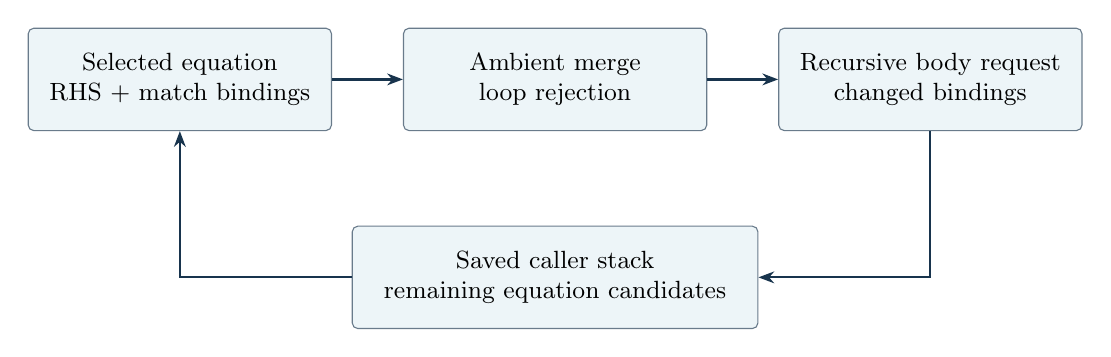
\begin{tikzpicture}
  \node[box] (candidate) {Selected equation\\RHS + match bindings};
  \node[box,right=9mm of candidate] (merge) {Ambient merge\\loop rejection};
  \node[box,right=9mm of merge] (body) {Recursive body request\\changed bindings};
  \node[wide,below=12mm of merge] (stack) {Saved caller stack\\remaining equation candidates};
  \draw[arr] (candidate) -- (merge);
  \draw[arr] (merge) -- (body);
  \draw[arr] (body.south) |- (stack.east);
  \draw[arr] (stack.west) -| (candidate.south);
\end{tikzpicture}
\end{center}
\diagramcaption{Local retained equation execution. The body returns through
the saved continuations; it does not replace its changed bindings by the
pre-call frame. This continuation law does not identify the fuelled HE and
explicit-scope LeaTTa query policies, or establish their full independent
recursive-source correspondence.}

Native retained execution supports pause, continuation, inspection and
cancellation. Checked readback components preserve contextual bindings and
distinguish pending computation from written syntax, under explicit
representation assumptions.

The general correspondence still needs arbitrary nesting, scope, quotation,
typed raw arguments, shared choices, branch worlds, demands, ownership,
effects and residuals. Flattened answer equality cannot establish this:
losing a binding world may change a later demand.

\sources{\name{Mettapedia/Languages/MeTTa/HE/RetainedArgumentSpecification.lean},
\name{Mettapedia/Languages/MeTTa/HE/ScopedEquationQuery.lean},
\name{Mettapedia/Languages/MeTTa/HE/LeaTTaScopedQuery.lean},
\name{Mettapedia/Languages/MeTTa/HE/FirstSuccessSourceExecution.lean},
\name{Mettapedia/Languages/MeTTa/HE/ReflectedStepSharing.lean},
\name{Mettapedia/Languages/MeTTa/Bridges/GSLT/CeTTaNeedHistory.lean},
\name{Mettapedia/Languages/MeTTa/Bridges/GSLT/CeTTaFrameWriteback.lean}.}
\scope{The model proofs and runtime controls are distinct evidence. They do
not constitute a complete theorem about compiled CeTTa execution, nor freeze
the eventual Prime candidate calculus.}

\newpage
\section{GSLT and rho: retain searches, publish occurrences}

The scoped GSLT scheduler advances actual premise, matcher and query frames.
It retains pending tasks, proved results and unresolved obligations.
PeTTa's authored program driver packages these searches into resumable jobs.
Its aggregate and publication are deliberately distinct: a later job may
already have results while an earlier incomplete job still controls their
public order.

\begin{center}
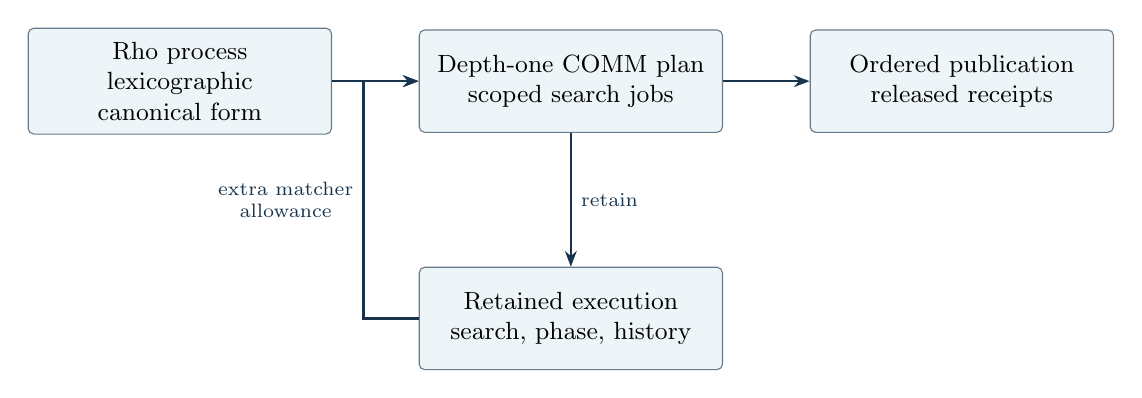
\begin{tikzpicture}
  \node[box] (proc) {Rho process\\lexicographic canonical form};
  \node[box,right=11mm of proc] (jobs) {Depth-one COMM plan\\scoped search jobs};
  \node[box,right=11mm of jobs] (pub) {Ordered publication\\released receipts};
  \node[box,below=17mm of jobs] (search) {Retained execution\\search, phase, history};
  \draw[arr] (proc) -- (jobs); \draw[arr] (jobs) -- (pub);
  \draw[arr] (jobs) -- node[hint,right]{retain} (search);
  \draw[arr] (search.west) -- ++(-7mm,0) coordinate (retry)
    -- node[hint,left]{extra matcher\\allowance} (retry |- jobs.west) -- (jobs.west);
\end{tikzpicture}
\end{center}

The actual \name{rho:run:resume-search} equation advances the pending
\name{ProgramObservation} and returns the full updated \name{RhoSearch}.
The evaluator-return and completion theorems cover that quoted equation,
including unchanged ambient state and empty effect queues.
\name{Search.resume_valid} retains earned validity, and publication grows
by prefix.

A released receipt supplies a source-valid rho step modulo structural
congruence. The existing \name{step_sound}, \name{step_quiescent} and saturation
results distinguish a step, quiescence and insufficient search allowance.
Empty publication establishes quiescence only when the search is complete.
Stopping with no answer so far is not evidence that there is no answer.

The shared trajectory law is instantiated by scheduled states and actual
PeTTa jobs/programs:
\[
 \resume(s,m+n)=\resume(\resume(s,m),n).
\]
The units differ: scheduled fuel counts ticks; PeTTa adds allowance per job.
Publication cursors emit only a newly released suffix and keep absolute
occurrence ordinals, including equal-valued duplicate answers.

\sources{\name{Mettapedia/OSLF/MeTTaIL/StructuralDescentScheduledExecution.lean},
\name{Mettapedia/Languages/MeTTa/PeTTa/Bridges/MeTTaIL/GeneralProgramResumptionExecution.lean},
\name{Mettapedia/Languages/MeTTa/PeTTa/Bridges/MeTTaIL/RhoRunnerExecution.lean}.}
Retained \name{Execution} adds successive completed COMM commitment and
cancellation to the search state. A commit selects one completed publication,
records its before/receipt/after triple, and begins a new search for the
successor process. Its quoted \name{rho:run:commit-candidate} equation checks the
entire supplied receipt wire against that local selection. A foreign candidate
or an immediate stale candidate does not extend the history. Resume preserves
the committed prefix; cancellation preserves history and drops live work.
\name{Execution.advance_add} instantiates the shared resumable trajectory.
Its fuel counts commit attempts, including no-ops; matcher allowance is resumed
separately. A two-communication control keeps both commits in chronology.

Every execution reached by any sequence of retained operations is sound
(\name{Retained.Reached.sound}): its history is a chronological sequence of
committed depth-one COMMs from the canonical start (\name{Retained.Reached.chain}),
its live search runs at that history's endpoint, and a done phase there is exact
quiescence. A commit placed at the wrong state, or with a result that is not the
receipt's, is not a chronicle. Under the common owned host
(\name{Retained.owned_publication}) committed COMMs reach the world exactly once,
copies of used tickets are refused, and the delivered history is that chronological
COMM sequence.

Selection need not always use the first published receipt.
\name{commitPublished} validates membership of the complete supplied receipt,
including its matcher, source job, bindings and premise history. Two ground
communications in disjoint multiset components construct a retained diamond
(\name{disjoint_retained_diamond}): each edge is an actual completed search
and licensed commit. Both schedules reach the same process; their chronological
histories remain distinct, with equality only under the declared causal observer.

The local dependency interface names input, output and fresh allocation
occurrences. Distinct keys retain distinct resources even when their process
values coincide. Fresh, live and spent states prevent reusing a consumed key.
The actual read program produces the candidate's dependencies; disjoint
read/write footprints prove that an unrelated commit preserves its validation.
\name{replay_after_history_refused} excludes reusing a consumed occurrence
through any later accepted history. Cancellation closes the owned publication
channel, and stale reads publish no world change even with a current ticket.
The quoted \name{rho:run:commit-published} and cell-store commands have source
execution and store-refinement proofs, as well as matching native controls.
An old whole-process search receipt is never relabelled for the successor:
its search is rebuilt there, while the local dependency certificate can survive
independent updates.

\scope{A commit's independent rho-step licence requires valid search and a
well-typed process. The quoted bridge uses the pinned depth-one COMM plan and
prepared encoded values. The owned host is a sequential model of authority;
durable or distributed exclusive delivery is a host obligation, and fairness over
all alternatives is not proved here.}

\newpage
\section{World queries: what can safely survive a change?}

A pure adaptive query can choose its next read from a previous result.
Its observation therefore contains both its answer and the ordered reads it
actually performed. A read certificate records complete values, including
absence and complete ordered match lists.

\begin{center}
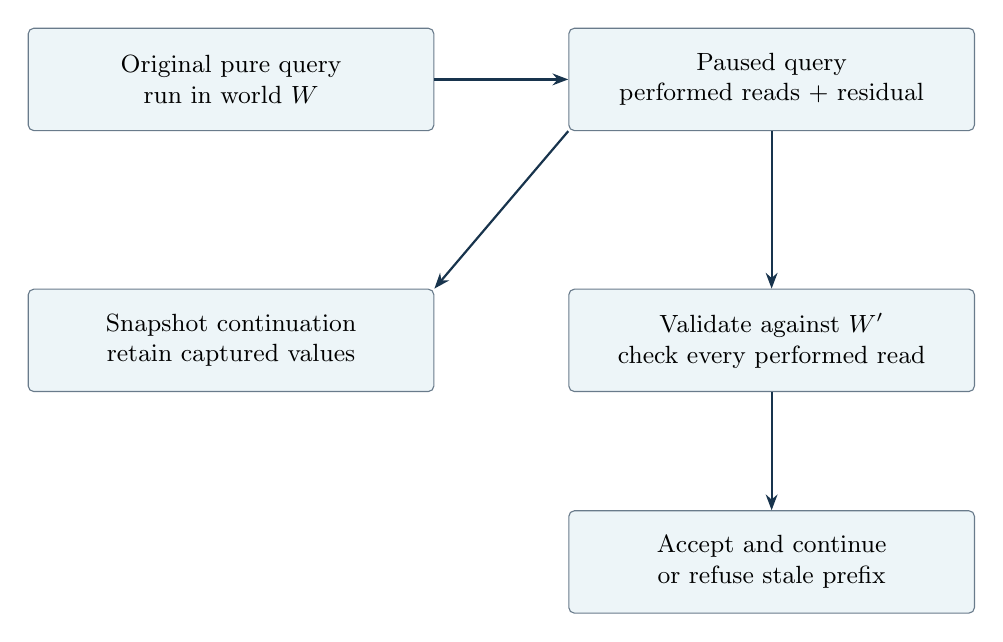
\begin{tikzpicture}
  \node[wide] (query) {Original pure query\\run in world $W$};
  \node[wide,right=17mm of query] (pause) {Paused query\\performed reads + residual};
  \node[wide,below=20mm of query] (snapshot) {Snapshot continuation\\retain captured values};
  \node[wide,below=20mm of pause] (validate) {Validate against $W'$\\check every performed read};
  \node[wide,below=15mm of validate] (continue) {Accept and continue\\or refuse stale prefix};
  \draw[arr] (query) -- (pause);
  \draw[arr] (pause.south west) -- (snapshot.north east);
  \draw[arr] (pause) -- (validate);
  \draw[arr] (validate) -- (continue);
\end{tikzpicture}
\end{center}

Suppose the query reads all matches at a key and gets $[a,a]$. Replacing that
list by $[a,a,b]$ changes the read even though both results are nonempty.
Replacing it by $[a]$ loses an occurrence. Reordering it can change a first
answer. An empty result must also be recorded: a later insertion invalidates
the earlier absence. An update to an unread key can remain compatible.

\name{run_eq_of_agrees} proves that agreement on the complete performed
certificate preserves the query's answer and read path.
\name{Retained.resumeValidated} checks the performed prefix before executing
any pending read. \name{Retained.validated_fresh} connects an accepted earned
prefix to fresh execution of the original query in the new world.

Snapshot continuation is a different policy. A residual may already have
closed over a captured answer, and retains it even when the current store
changes. Failed validation does not retroactively turn that old residual into
a fresh query. Starting the original pure query again is possible; replaying
committed effects to refresh knowledge needs a separate effect contract.

Writes computed from reads follow the same rule. An owner runs a transaction,
a pure query whose answer is a list of writes, on the snapshot it saw and proposes
the writes with the complete read certificate. The ledger commits the proposal
only when every recorded read agrees with the current store. An accepted proposal
writes what its transaction would write now (\name{commit_fresh}), so accepted
commitments are serializable (\name{commitAll_serial}); a proposal is refused
exactly when one of its reads changed (\name{commit_refused_iff}). Two increments
of one counter from the same snapshot commit once; rerunning the refused one on a
fresh snapshot commits it; writing both blindly loses an update. The ledger is a
retained state for the owned host, which publishes each accepted write list once
(\name{ledger_published_once}).

\sources{\name{Mettapedia/Machines/ReadOnlyQuery.lean},
\name{Mettapedia/Machines/ReadCertifiedQueryReuse.lean},
\name{Mettapedia/Machines/ValidatedCommit.lean},
\name{Mettapedia/Coalgebra/CoherentPrefixTower.lean}.}
\scope{This is a pure read interface. Query identity, program revisions,
ownership and service authority are additional dependencies; an unchanged
read list alone does not validate a changed program or authorize consumption.}

\newpage
\section{Effects, services and the limit of a copied continuation}

An effect session retains an actual driver residual, the current interpreted
world, and its committed event history. Continuing advances the residual and
interprets only the new event suffix. Splitting a budget preserves all three
components, including when the handler performs a non-idempotent increment.

\begin{center}
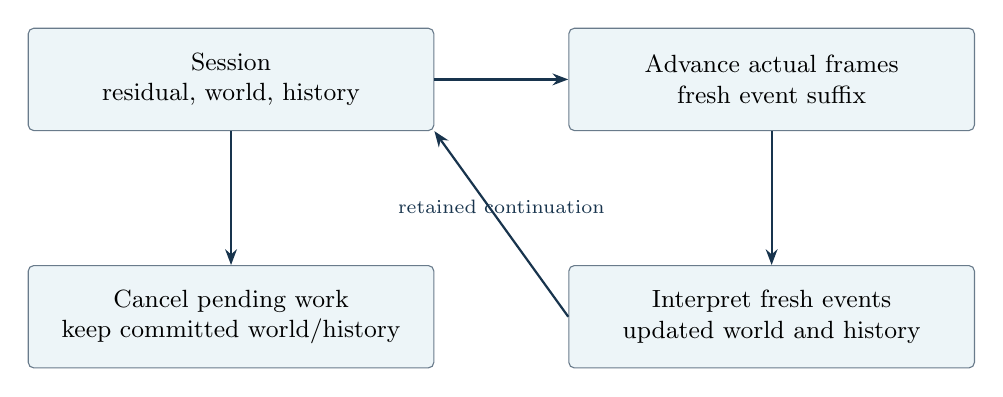
\begin{tikzpicture}
  \node[wide] (session) {Session\\residual, world, history};
  \node[wide,right=17mm of session] (advance) {Advance actual frames\\fresh event suffix};
  \node[wide,below=17mm of advance] (commit) {Interpret fresh events\\updated world and history};
  \node[wide,below=17mm of session] (cancel) {Cancel pending work\\keep committed world/history};
  \draw[arr] (session) -- (advance); \draw[arr] (advance) -- (commit);
  \draw[arr] (commit.west) -- node[hint,above]{retained continuation} (session.south east);
  \draw[arr] (session) -- (cancel);
\end{tikzpicture}
\end{center}

The independent recursive \name{Runs} relation supplies the meaning of
children and caller continuations. Explicit frames realize that meaning with
the exact ordered trace. \name{Session.resume_add} gives the complete sliced
state law. \name{Session.cancel} discards pending execution and preserves
the committed world/history; later resumes stutter.

Pairwise commuting actions permit a permutation theorem for the final world.
The ordered trace still records a different schedule. A negative control
shows a reversed noncommuting pair changes the world. Commutation must be
proved for the actual actions and interference conditions.

The general event machine also has resumable service handling. A request can
run another machine while retaining the caller and service continuations;
faults, stuck endpoints and divergence remain distinct from replies. This is
related to the handler-as-computation approach of interaction trees~\cite{ITrees};
the present interface uses explicit states and finite budgets.

\subsection*{Owned interaction}
The pure session and cursor laws do not enforce exclusive ownership: copying an
earlier cursor can redeliver, and restarting a program can repeat an increment.
The owned host adds consuming authority. A retained computation begins under a
ticket; submitting its derived actions consumes the ticket, applies the actions
once to the shared world and issues the successor ticket. A used ticket is refused
(\name{Owned.used_ticket_refused}), so copies of a computation act at most once
(\name{Owned.copies_act_once}); a cancelled computation refuses further work,
private forks never touch the shared world, and every reached host state accounts
its world as the initial world under the delivered actions. For commuting actions
the final world does not depend on the interleaving (\name{interpret_commute_past},
\name{interpret_interleaving}); a noncommuting pair is a negative control.
External crash recovery, durable exactly-once delivery and the disposition of
non-droppable obligations need a service protocol beyond this sequential host.

\sources{\name{Mettapedia/Machines/OwnedPullDriver.lean},
\name{Mettapedia/Machines/ExecutionHistoryReadout.lean},
\name{Mettapedia/Machines/ResourceOwnership.lean},
\name{Mettapedia/GSLT/Distinction/ProductiveBlocks.lean}.}

\newpage
\section{The fixed C-language machine}

The fixed core is a source language over the existing C11 semantic modules:
typed integer operations under a selected integer model and signed-conversion
policy, byte memory with effective types, automatic object scopes and array
pointers. Names resolve through the lexical scopes of the current activation.
Pure expressions read integer elements, compute, take addresses and move pointers
within live arrays. Statements assign through places, set pointer variables, call
functions recursively with parameter objects, return values, branch, loop, break
and continue, open blocks that reserve declared objects and retire every owned
lifetime on every exit, allocate and release dynamic objects, and suspend on
external requests.

\begin{center}
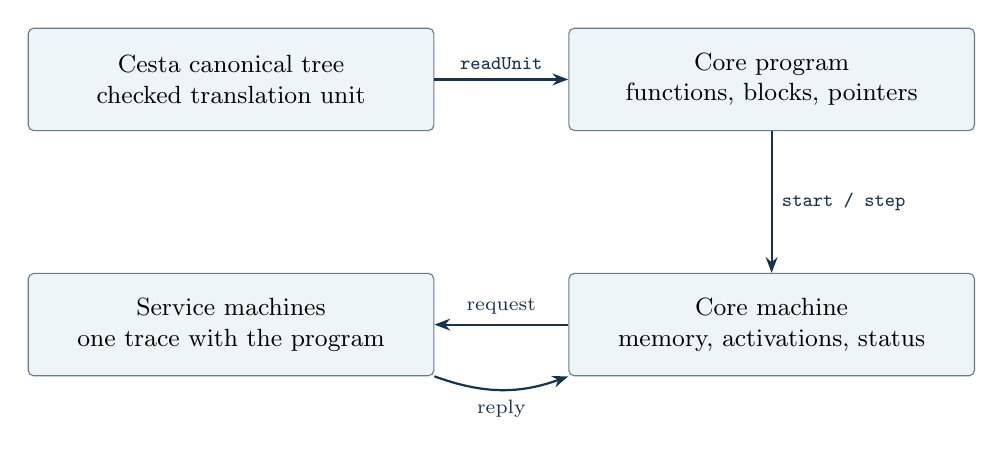
\begin{tikzpicture}
  \node[wide] (ast) {Cesta canonical tree\\checked translation unit};
  \node[wide,right=17mm of ast] (core) {Core program\\functions, blocks, pointers};
  \node[wide,below=18mm of core] (machine) {Core machine\\memory, activations, status};
  \node[wide,below=18mm of ast] (service) {Service machines\\one trace with the program};
  \draw[arr] (ast) -- node[hint,above]{\texttt{readUnit}} (core);
  \draw[arr] (core) -- node[hint,right]{\texttt{start / step}} (machine);
  \draw[arr] (machine.west) -- node[hint,above]{request} (service.east);
  \draw[arr] (service.south east) to[out=-20,in=-160] node[hint,below]{reply} (machine.south west);
\end{tikzpicture}
\end{center}

The executable step is sound and complete for an independent step relation whose
premises are the memory, scope and expression judgments (\name{step_iff}), up to the
two choices C11 leaves open: the identity of each new object and whether an
allocation succeeds. Undefined behaviors stop with their reason: arithmetic
overflow or division by zero, an access to a dead, indeterminate, out-of-bounds or
misaligned element, a trap representation, a pointer formed outside its array, an
invalid or repeated release, or a used missing return. A constraint violation and
a failed host service are reported separately. As a common event machine the core
publishes each step as an occurrence with its actual configurations, and budget
slicing resumes the retained configuration exactly.

The Cesta reader is a static checker for the core fragment. Names resolve through
the C block scopes, operands are integers or pointers to a declared integer type,
and calls are checked against the signatures of the program's functions and of the
host's services. Interleaved declarations become nested blocks; \code{E1[E2]},
\code{&*E} and \code{&E1[E2]} follow their C11 equivalences; returned values and
service arguments are converted to the declared types; the end of \code{int main}
returns \code{0}. Every reading function is equivalent to an independent reading
relation (\name{readUnit_iff}). Constructs outside the fragment are refused, not
approximated. Sources parsed by the Cesta binary run on the core to the values GCC
and Clang compute. On the undefined controls, AddressSanitizer and
UndefinedBehaviorSanitizer report the use after scope, use after release, double
release and overflow under both compilers; only Clang reports the pointer formed
past its array.

Requests are served by service machines through the common callback protocol
(\name{served_call}); running services as machines is a compilation stage from
atomic answers (\name{servedStage}). With the retained HE evaluator as the service,
a C loop calling a MeTTa function returns what GCC computes for the same loop over a
C definition, and the trace contains exactly the evaluator's result occurrences
(\name{metta_call_publishes_evaluator_meaning}). Several results, or an unreadable
one, stop the program with the service's fault: a reply never selects one result
from several.

The located layer remains the place for side effects inside expressions. Its
expression scheduling makes full-expression boundaries and unsequenced conflicts
explicit, and \name{StatementExecution.execute_iff} connects its executable
transition to independent rules.

The common fixed/located fragment now has a constructed translation. An
executable lowering agrees with an independent admission relation for arbitrary
finite pure expressions and for assignment, conditionals, loops, break,
continue and return. Pure expression schedules preserve the same scalar and
semantic memory. An assignment additionally executes its actual conversion,
store and returned-value occurrences. Both legal store/result orders reach
the same boundary; neither may bypass an unfinished operand.

\name{statement_step_simulation} and \name{control_step_simulation} replace
one fixed-core control step by its actual located expression and boundary
steps. Their finite-history composition covers arbitrary admitted successful
runs. \name{Block.finished_realization} then executes the final verdict on the
existing budgeted runner and retains the complete receipt list and unused
schedule suffix. The common memory relation preserves object allocation and
lifetime headers as well as contents; reads outside their admitted live
catalogue are refused. A counter loop reaches zero with the committed values
$[2,1,0]$ under both store/result policies.

Different legal evaluation orders can encounter different first faults when
both pure operands fail. The cross-layer observer therefore distinguishes a
defined scalar result from failure without identifying those diagnostics.
Each located execution retains its own exact fault and chronological prefix.
The whole-run reverse construction now discovers the owning source control
through every partial expression and assignment history. Its
\name{ReachedControl.step} either constructs a genuine source step or strictly
decreases finite pending-expression work. Thus arbitrary source loops remain
possible while an infinite stretch of source-free administration is excluded.
\name{terminal_observation_iff} proves preservation and reflection of complete
success or refusal under the admitted scheduler. The schedule license checks
the actual next ready occurrence; an unready operation is malformed scheduling,
not source undefined behavior. \name{ReachedControl.run} additionally retains
the earned source prefix and exact receipts at every budget exhaustion and
selection request. No supplied decomposition into source blocks is required.

\sources{\name{Mettapedia/Languages/C11/FixedCore.lean},
\name{Mettapedia/Languages/C11/FixedCoreStatements.lean},
\name{Mettapedia/Languages/C11/CestaFixedCore.lean},
\name{Mettapedia/Languages/C11/FixedCoreServices.lean},
\name{Mettapedia/Languages/MeTTa/HE/RecursiveService.lean},
\name{Mettapedia/Languages/C11/LocatedStatements.lean},
\name{Mettapedia/Languages/C11/StatementExecution.lean},
\name{Mettapedia/Languages/C11/ExpressionEventHistory.lean},
\name{Mettapedia/Languages/C11/StatementMachineRefinement.lean}.}
\scope{Object layouts are the selected ABI's, an explicit parameter; pointer
variables hold an abstract provenance-carrying value; external services answer each
request at most once. Named extensions outside the core include calls inside
expressions, pointer-typed objects in byte memory, structures, floating types,
\code{for}, \code{do}, \code{switch} and \code{goto}, array initializers, function
pointers and threads. The common-fragment translation does not additionally
cover calls, allocation instructions or side-effecting operands. These remain
available only at their separately specified machine boundaries.}

\newpage
\section{Regional machines and explicit crossings}

A useful machine comparison fixes three things: a region of admitted programs,
the observations to preserve, and the resource objective. Removing an
observation can permit more representations, but does not by itself establish
a faster implementation. Operational accounts and measured native costs are
different claims.

\begin{center}
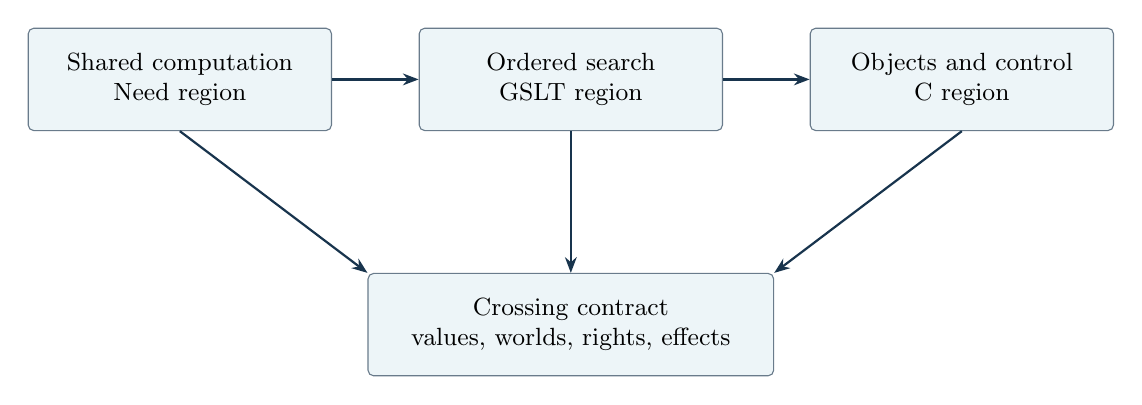
\begin{tikzpicture}
  \node[box] (need) {Shared computation\\Need region};
  \node[box,right=11mm of need] (search) {Ordered search\\GSLT region};
  \node[box,right=11mm of search] (c) {Objects and control\\C region};
  \node[wide,below=18mm of search] (contract) {Crossing contract\\values, worlds, rights, effects};
  \draw[arr] (need) -- (search); \draw[arr] (search) -- (c);
  \draw[arr] (need.south) -- (contract.north west);
  \draw[arr] (search) -- (contract);
  \draw[arr] (c.south) -- (contract.north east);
\end{tikzpicture}
\end{center}

A crossing states what is translated, which observer is preserved, what
dependency/authority evidence travels, and how return or refusal behaves.
Pairwise agreement is insufficient for arbitrary networks: composed paths
must satisfy the applicable compatibility laws. Existing gluing results cover
equation models over a shared binding algebra, equivalence-valued view systems
with trivial cycle transport, and compatible causal histories with explicit
read/write and observation hazards. None of these identifies arbitrary guest
logics or supplies their complete native execution. A general sheaf account of
regional machines still needs its actual restriction and gluing maps.
Trivial cycle transport concerns changes of view that claim to preserve the
same object. An effectful computation cycle can change the world and emit
events; it is not such an identity transport.

\subsection*{Observation, demand and retention are separate controls}
An observer chooses what distinctions a user sees. Demand chooses how much
work is requested. Retention chooses what remains available for inspection or
continuation. \code{once} and \code{select k} bound requested successful
occurrences; they are not general permission to erase faults, reorder effects
or discard owned pending work. Zooming out can license a coarser readout;
zooming in later is possible only if the required information was retained.

\subsection*{Machines do not impose one universal logic}
Conversion within one shared logic and transport between distinct logical
guests have different contracts. A selected machine family retains each
kernel's own state and question type. It does not make HOL, dependent type
theory and set theory one calculus. A stable guest can remain stable while
Prime's candidate develops, provided the crossings state their assumptions.

ZINC~\cite{ZINC} is useful historical comparison for an ML implementation.
Here ZAM denotes a \emph{zipper abstract machine}, which is a different idea
and is discussed in Section~\ref{sec:holes}. No general WAM optimality theorem
is claimed. New regional machines can be
derived or compared through these interfaces, then judged by correspondence
and an explicit cost model.

\scope{The integration target is faithful higher-order MeTTa execution.
CAM and the fixed C core supply substantial instances and reusable laws;
they do not displace that language-facing purpose.}

\newpage
\subsection{Modules, presentations and necessary machine state}

A module assembles declarations and their selected policy layers. A GSLT
states their operational meaning. A regional machine realizes that meaning
with its own representation and control. These are distinct objects: joining
declarations neither selects an evaluation strategy nor proves that two
machines can interact safely.

Universality and the absence of a globally best optimizer do not determine
how many machine families an implementation must expose. One interpreter can
itself dispatch among several strategies. Regional specialization is justified
by a stated program region, correspondence and resource objective, rather
than inferred from undecidability alone.

A region can support a portfolio of implementations, including difficult
higher-order regions; it need not have one fixed algorithm. Vampire provides
an operational precedent for scheduling configurable proof strategies from
workload features~\cite{DynamicStrategyPriority}. The existing bounded-search
portfolio retains private batches, distinguishes cutoff from exhaustion and
publishes one strategy's batch. Combining strategies' rediscovered answers
would require a separate occurrence correspondence. Fair scheduling alone
does not certify exhaustion after a finite budget.

Constraint-solving backends are also candidates for finite collection
matching. A checked encoding must relate decoded solutions to the declared
source matches, preserving their occurrence identities. Auxiliary Boolean
assignments need not correspond one-to-one with those matches, so ordinary
model counting does not automatically count semantic answers. SAT witnesses
and checked unsatisfiability certificates can justify different conclusions;
the encoding and coverage obligations remain~\cite{LRAT}. Specialized AC
representations can also be effective for important restricted rule
classes~\cite{EkerAC}. The general complexity bound does not choose the best
implementation for a workload.

\begin{center}
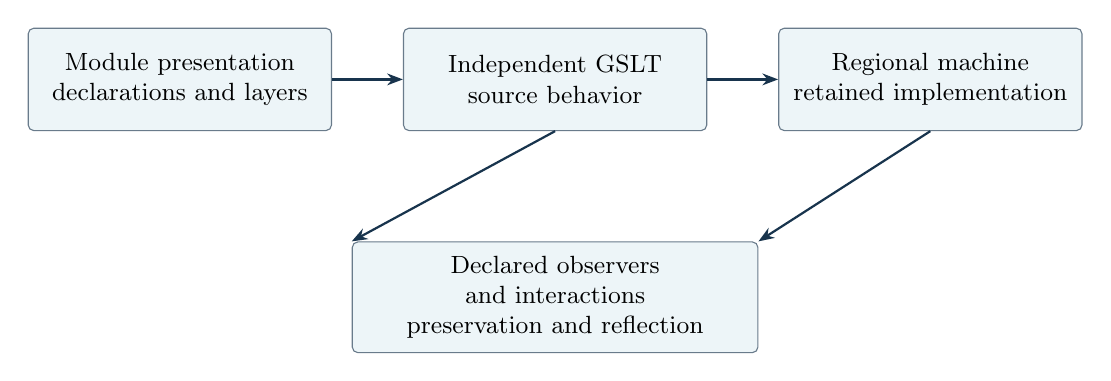
\begin{tikzpicture}
  \node[box] (module) {Module presentation\\declarations and layers};
  \node[box,right=9mm of module] (gslt) {Independent GSLT\\source behavior};
  \node[box,right=9mm of gslt] (machine) {Regional machine\\retained implementation};
  \draw[arr] (module) -- (gslt);
  \draw[arr] (gslt) -- (machine);
  \node[wide,below=14mm of gslt] (observer) {Declared observers and interactions\\preservation and reflection};
  \draw[arr] (gslt.south) -- (observer.north west);
  \draw[arr] (machine.south) -- (observer.north east);
\end{tikzpicture}
\end{center}

An admitted execution region restricts a backend's qualification, not the
module format. A first-order backend can refuse a presentation containing
binders while retaining that presentation for a suitable scoped interpreter.
A general interpretation path and its specialized realizations should share
an independent source observation; the existence of that path does not by
itself establish coverage of every binder or premise form.

The presentation and its surface syntax also have different responsibilities.
The existing five-field \name{LanguageDef} carries sorts, constructors,
equations and rewrites; \name{ExtendedLanguageDef} attaches independently
authored dependent layers. A proof calculus is one such layer. Several concrete
syntaxes can elaborate to this shared structure. Upstream syntax is an
interchange route, not a requirement that every local extension fit a
historical grammar. Improvements to notation must preserve binding, declaration
origins and the laws of the selected layers.

Four current boundaries must not be conflated: the closed-theory
\name{moduleTheory!} Lean quotation; the structured \name{module/1} envelope;
textual \name{.module} languages; and the live runner's emitted MeTTa program.
The quotation and envelope already have structural elaboration laws. The
runner's \name{ReadAfterRender} theorem concerns MeTTa program text, not the
upstream module grammar. A canonical portable surface now establishes
\[
  \mathsf{readBytes}\bigl(\mathsf{renderBytes}(P)\bigr)
    =\mathsf{some}(P),
\]
with a separate elaboration theorem into the existing assembled presentation.
The character reader uses the existing lexer/parser/atom-reader pipeline;
the byte reader validates UTF-8. The complete finite \name{LanguageDef}
codec retains binders, collection metadata, equations and scoped premises.
Dependent layers carry an explicit indexed codec; proof calculi, export
names and products are concrete instances. This does not claim that every
Lean function or relation has a finite serialization.

The surface is an inert \code{(module:document payload)} declaration.
Origin-bearing entries survive the text boundary before the existing import
contract decides sharing or collision. Unknown envelope payloads remain data;
a declared layer rejects an incompatible schema. The canonical syntax does
not implement a historical upstream grammar. Preserving comments, formatting
and import expressions still requires a separate source representation:
an assembled presentation cannot reconstruct information it has discarded.

A finite rule list need not imply first-order syntax: its rules can have
binders and higher-order premises. An effectively enumerable rule family
additionally needs a finite generator description and evidence for each
selected instance. An arbitrary semantic relation in Lean's abstract
\name{GSLT} record need not be effectively enumerable or serializable.
Keeping that semantic generality is compatible with requiring explicit
presentation and realization evidence at an executable boundary.

Even a simple specialization must carry the typing boundary. A variable-root
rule $x:\mathsf{Nat}\rightsquigarrow\mathsf{zero}$ structurally matches a
Boolean term if its type is forgotten. Checked invocation-sort selection must
exclude that candidate before execution, retaining the original indices of
later rules. Comparing two untyped implementations would miss this error.
The same contract must fix when query inputs become available. In the checked
provider profile considered here, an output of the current query does not
retroactively satisfy a required input to that query.

The question of necessary state is relative to the admitted observations and
future interactions. Write
\[
 s\approx_{O,\mathcal C}t
 \quad\Longleftrightarrow\quad
 \forall C\in\mathcal C,\quad O(C[s])=O(C[t]).
\]
The observation may include outcomes, residuals, effects or probability laws.
An encoding supporting every such interaction cannot identify states outside
this equivalence. Turning it into a machine quotient additionally requires
stability under the actual transitions and contexts. This identifies necessary
distinctions, not a fastest implementation or a computable finite quotient.

The contextual observed-coalgebra owner constructs a quotient, its transition
square and exact factorization for compatible natural consumers. That owner
uses labelled set-valued futures: order, multiplicity and probability require
their additional representations and laws. Its quotient is not already the
complete MeTTa machine. The ordered-machine bridge also reads an ordered
successor list as a GSLT membership relation; that modal view alone forgets
list order and repeated successors.
Occurrence simulations transport these ordinary modal formulas without a
positional alignment. The converse fails for occurrence preservation: a
one-successor machine and a machine with two equal successor occurrences
satisfy the same formulas, while their occurrence bags have different
cardinality. This limitation is proved in the native-type bridge.

\begin{center}\small
\begin{tabularx}{\textwidth}{@{}>{\raggedright\arraybackslash}p{36mm}
  >{\raggedright\arraybackslash}X>{\raggedright\arraybackslash}X@{}}
\toprule
Admitted region & Useful machine structure & Distinction to preserve\\
\midrule
Functional terms & CEK, Krivine, CAM or Need & Strategy, captured environment, shared demand\\
Rule search & Retained matcher and frontier & Occurrence identities, selected traversal, residual work\\
Reflective processes & Communication/reaction machine & Names, quotation, ports, permitted scheduling\\
Certificate checking & Decoder, proof state and snapshot & Declared theory, references, checked evidence\\
Probabilistic programs & Kernel-valued machine and history & Draw identity, scores, captured random values\\
\bottomrule
\end{tabularx}\end{center}

Algebraic operational semantics connects syntax and behavior through a
distributive law when the required rule-format and categorical hypotheses
hold~\cite{TuriPlotkin}. Polynomial syntax alone does not provide that law.
Likewise, module-join compatibility is distinct from preservation of conversion
or effects. The existing first-match priority counterexample fails substitution
stability; ordinary relational rewriting has its own substitution theorem.

\sources{\name{Mettapedia/GSLT/LanguageDef/ModuleAlgebra/Semantics.lean},
\name{Mettapedia/GSLT/LanguageDef/ExtendedLanguageDef.lean},
\name{Mettapedia/GSLT/LanguageDef/ModuleAlgebra/UpstreamTheoryQuotation.lean},
\name{Mettapedia/GSLT/LanguageDef/ModuleFormat/Authoring.lean},
\name{Mettapedia/GSLT/LanguageDef/ModuleFormat/Text.lean},
\name{Mettapedia/GSLT/LanguageDef/ModuleFormat/Portable.lean},
\name{Mettapedia/Languages/MeTTa/PeTTa/Bridges/MeTTaIL/GeneralLiveRunnerEmission.lean},
\name{Mettapedia/Machines/BoundedSearchPortfolio.lean},
\name{Mettapedia/GSLT/Logic/ContextualObservedCoalgebraQuotient.lean},
\name{Mettapedia/OSLF/Framework/OrderedSystemNativeTypes.lean},
\name{Mettapedia/GSLT/Dedukti/LeanMinusPriority.lean}.}

\newpage
\subsection{Staged lowering and runtime interaction}

There are two different ways for one language machine to use another.
\emph{Staged lowering} transforms the source before execution.
\emph{Runtime interaction} keeps both computations alive across requests and
returns. Both need semantic preservation, but they retain different states.
Operational semantics based on explicit language boundaries is established
work~\cite{MultiLanguage}; hygienic macro binding also has its own semantic
models~\cite{ScopeSets}.

\begin{center}
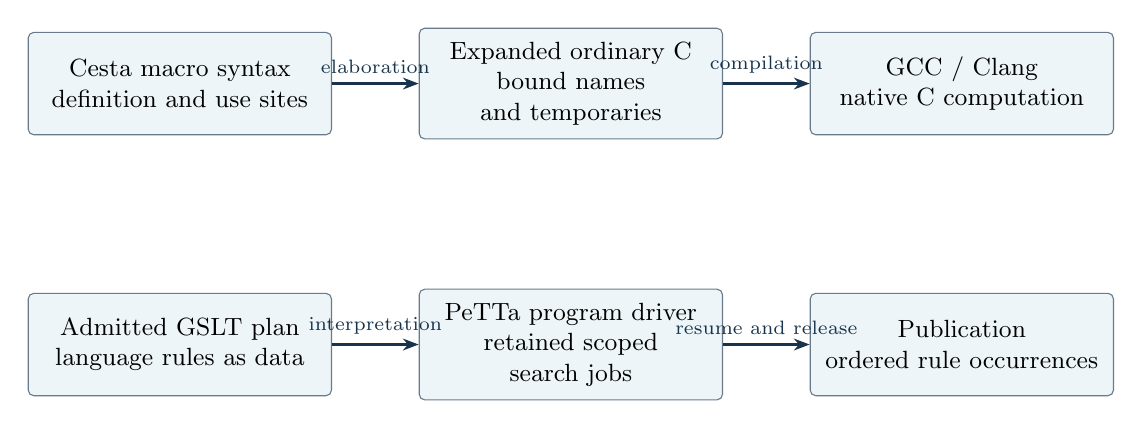
\begin{tikzpicture}
  \node[box] (macro) {Cesta macro syntax\\definition and use sites};
  \node[box,right=11mm of macro] (expanded) {Expanded ordinary C\\bound names and temporaries};
  \node[box,right=11mm of expanded] (native) {GCC / Clang\\native C computation};
  \draw[arr] (macro) -- node[hint,above]{elaboration} (expanded);
  \draw[arr] (expanded) -- node[hint,above]{compilation} (native);
  \node[box,below=20mm of macro] (presentation) {Admitted GSLT plan\\language rules as data};
  \node[box,right=11mm of presentation] (jobs) {PeTTa program driver\\retained scoped search jobs};
  \node[box,right=11mm of jobs] (receipts) {Publication\\ordered rule occurrences};
  \draw[arr] (presentation) -- node[hint,above]{interpretation} (jobs);
  \draw[arr] (jobs) -- node[hint,above]{resume and release} (receipts);
\end{tikzpicture}
\end{center}

Cesta's current macro engine instantiates templates, resolves explicit binding
origins, introduces fresh locals, and emits C. Argument metadata distinguishes
syntax, values and modifiable places, with evaluation contracts. For the
checked narrowing library, source and target types are syntax; the input value
and output place are evaluated once by the emitted C. Macro expansion does not
execute the input expression. The native compiler supplies active-header name
inventory and checks the final C. This is a staged language layer; it is not an
extra interpreter running beside the resulting native program.

The current GSLT driver instead retains a licensed request and actual search
state for every job. Requests carry the presentation/environment, permissions,
binding context, expected type, source and physical rule/site identity.
Receipts retain matcher choices, captured and completed assignments, premise
history, and local and reconstructed targets. The quoted authored equations
are connected to PeTTa evaluation. The general target-step theorem requires
an equation-free, checked-stratified plan and sufficient search allowance.
Its exact canonical reduct-list theorem has a narrower root query-profile
scope. A presentation emitter and a general whole-run loop still need their
complete integrated proofs.

Treating an expander as an abstract machine can clarify its own binding and
phase semantics. It does not require paying for that machine at program runtime:
justified lowering can remove it. A live heterogeneous computation needs
runtime crossing rules in addition to staged source transformations.

\sources{\name{Mettapedia/GSLT/LanguageDef/MacroTemplateNames.lean},
\name{Mettapedia/GSLT/LanguageDef/MacroDefinitionPorts.lean},
\name{Mettapedia/GSLT/LanguageDef/MacroCheckedNarrowing.lean},
\name{Mettapedia/Languages/MeTTa/PeTTa/Bridges/MeTTaIL/GeneralProgramDriverExecution.lean}.}

\newpage
\subsection{A computational-metagraph machine as a candidate}

A candidate Meta-MeTTa machine would retain regional computations at nodes
and pending crossings at edges. Admission, transfer, advancement, reply,
refusal, cancellation and dependency validation would be explicit steps.
This heterogeneous machine remains an integration target.

\begin{center}
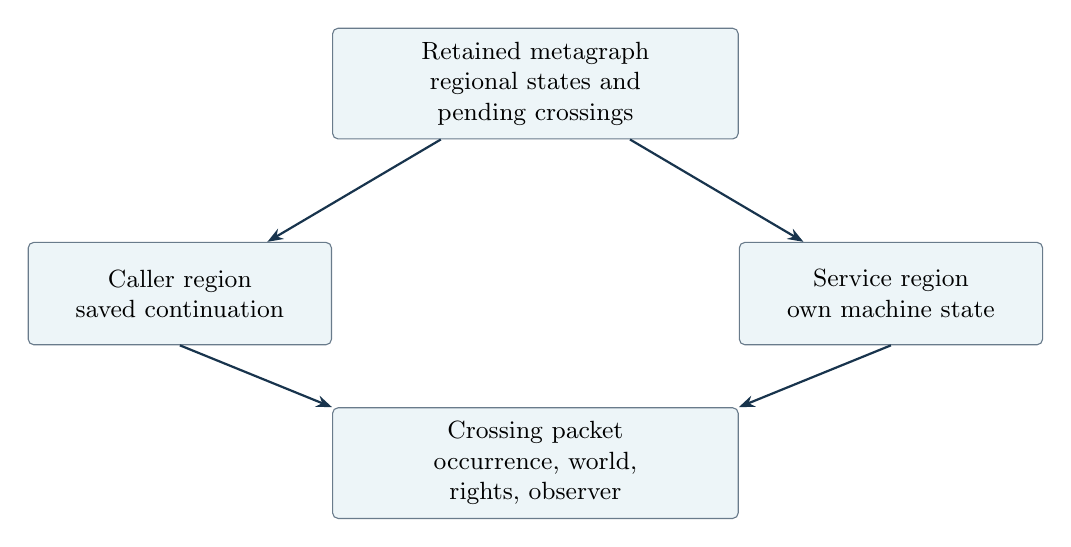
\begin{tikzpicture}
  \node[wide] (graph) {Retained metagraph\\regional states and pending crossings};
  \node[box,below left=13mm and 0mm of graph] (caller) {Caller region\\saved continuation};
  \node[box,below right=13mm and 0mm of graph] (service) {Service region\\own machine state};
  \node[wide,below=12mm of graph,yshift=-22mm] (edge) {Crossing packet\\occurrence, world, rights, observer};
  \draw[arr] (graph) -- (caller); \draw[arr] (graph) -- (service);
  \draw[arr] (caller.south) -- (edge.north west);
  \draw[arr] (service.south) -- (edge.north east);
\end{tikzpicture}
\end{center}

The state needs continuations, ordered occurrences, dependency evidence,
consuming authority and committed history. Each crossing must realize an
independent semantics preserving the selected observations.

\name{MachineCore.familyCore} retains heterogeneous state/question types but
cannot change the selection. \name{Machine.handle} constructs interaction
with retained caller and service states. \name{ScheduledFrontier} preserves
occurrence slots across differing completion times, under independence
hypotheses. Publication, read-validation and effect-session laws still need
the common ownership join.

\name{GSLT.Poly.BindingSignature} represents binding terms as a context-indexed
free monad. The indexed polynomial client in \name{GSLT.Poly.SortedTraversal}
retains argument occurrences and reply slots. Neither polynomial structure nor
a slot determines a child's interpretation or force rights.

In the MM2 evidence-material theory, two actual matcher paths conclude the
same fact but deliver different origin lists. Their consuming continuation
cannot factor through conclusion support. An ordered material batch or receipt
retains enough information; the recovery theorem uses a classical partial
inverse, rather than an executable native decoder.

Native MM2 controls separately run a finite staged consumer on three input
occurrences, two with equal payloads. Shared choice gives six deliveries;
separate choice coordinates give twelve. Sequence fields recover their order.
Retained cursors preserve the answers and three counter updates across reloads.
Restarting repeats an update; changing the captured environment changes later
answers. \code{head 1} alone still permits sibling writes. This does not
establish a general MeTTa correspondence or external-effects protocol.

Producer identity supports sharing; delivery identity supports occurrence
observation. Indexed set storage can retain both views. The richer encoding
then carries the surrounding machine's cursor, world and commitment protocol.

\sources{\name{Mettapedia/Machines/MachineSubstrate.lean},
\name{Mettapedia/GSLT/Distinction/ProductiveBlocks.lean},
\name{Mettapedia/GSLT/Distinction/OrderedSimulationSpans.lean},
\name{Mettapedia/GSLT/Distinction/CausalGluing.lean},
\name{Mettapedia/GSLT/Scope/Holonomy.lean},
\name{Mettapedia/GSLT/LanguageDef/ModuleAlgebra/SemanticGluing.lean},
\name{Mettapedia/GSLT/Poly/SortedTraversal.lean},
\name{Mettapedia/GSLT/Logic/ProgrammableSpaceMM2EvidenceMaterial.lean}.}

\newpage
\subsection{The trinity as a fibred web of presentations}

The language-facing trinity names intensional mathematics, extensional
mathematics and a GSLT-IL operation presentation. These are semantic roles,
not necessarily separate kernels. The contextual computational-trinity
framework compares programs, proofs or typed terms, and generalized elements
in spaces. Each face is a presheaf over contexts, so substitution is part of
the presentation rather than an untracked surrounding operation.

\begin{center}
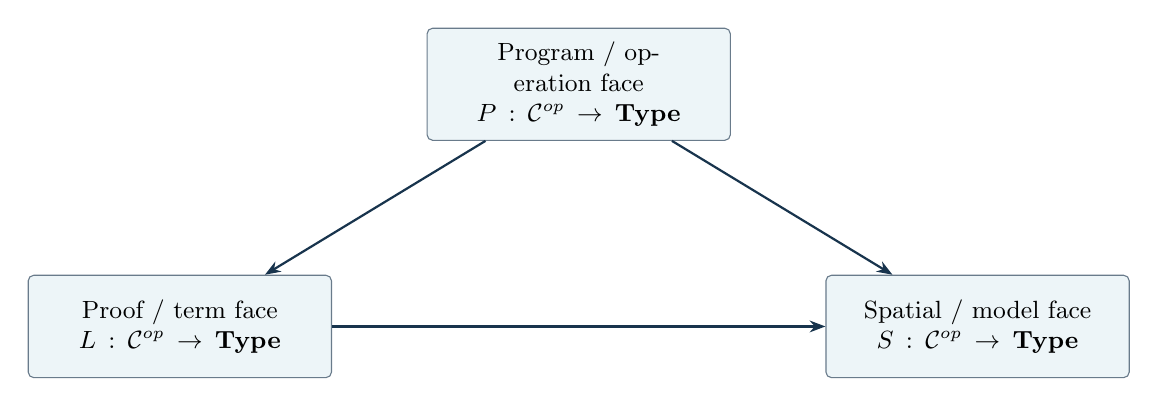
\begin{tikzpicture}
  \node[box] (program) {Program / operation face\\$P:\mathcal C^{op}\to\mathbf{Type}$};
  \node[box,below left=17mm and 12mm of program] (logic) {Proof / term face\\$L:\mathcal C^{op}\to\mathbf{Type}$};
  \node[box,below right=17mm and 12mm of program] (space) {Spatial / model face\\$S:\mathcal C^{op}\to\mathbf{Type}$};
  \draw[arr] (program) -- (logic);
  \draw[arr] (program) -- (space);
  \draw[arr] (logic) -- (space);
\end{tikzpicture}
\end{center}
\diagramcaption{Comparison means a commuting triangle of natural maps.
Exactness additionally requires invertible maps. The abstract construction
does not instantiate the whole native DTT/HOL/set/GSLT triangle.}

Actual categorical owners already have different variances. Theory models
reindex by reducts along theory arrows, forming a Grothendieck fibration.
Typed open code has forward transport and cocartesian lifts. Finite retained
execution paths form another category-valued index. These constructions do
not make every theory arrow an executable, resource-safe or conservative
machine crossing. The complete step, residual and observer comparison must
be added for the actual route. The additive world-model doctrine likewise
cannot silently justify deleting a record or normalizing a Bayesian update.

The STT/DTT and selected set-family bridges are scoped interpretations.
Representing a HOL formula does not prove it; a native inhabitant is not
automatically a source HOL derivation. Logical borrowing needs the selected
conservativity contract. Adding a stronger conversion bubble also needs its
own substitution and join laws. Two component normalizers do not necessarily
decide their combined conversion.

Hyperset presentations retain graph occurrences; material equality quotients
by bisimulation. A dependent consumer therefore needs family and section
descent before those distinctions are erased. Internal coalgebraic membership
and the host's well-founded membership remain distinct. Initial/final
comparisons also keep their bounds and existence hypotheses: identifying an
initial algebra with a final well-founded coalgebra does not prove that every
set functor has either~\cite{WellPointed}. Unrestricted powerset has no
set-sized fixed point. Qualified bounded constructions state their size
conditions separately.

\sources{\name{Mettapedia/Computability/ComputationalTrinity.lean},
\name{Mettapedia/GSLT/LanguageDef/TheoryGraphModels.lean},
\name{Mettapedia/Languages/MeTTa/PrimeCandidates/ContextualDataFibration.lean},
\name{Mettapedia/GSLT/Core/OperationalPathFibration.lean},
\name{Mettapedia/TypeTheory/MaterialSets/Hypersets/FamilyDescent.lean},
\name{Mettapedia/Logic/WorldModel/Indexed/Doctrine.lean}.}

\newpage
\section{Proof machines: scoped, licensed composition}
\label{sec:checking}

\begin{quote}
\emph{What follows from what, under which conditions?}
\end{quote}

A checking machine makes a proposed answer to this question inspectable.
The local rules specify the permitted connections; evidence identifies the
connection being proposed; composition connects its output to the next input.
The interface shared by proof checking and rewrite checking is therefore
\emph{scoped, licensed composition}. This identifies a common organization,
while leaving each presentation responsible for its own judgments, equality,
binding and resource rules.

Write
\[
 T;\Gamma\vdash e:A\longrightarrow B
\]
for a supplied piece of evidence $e$ connecting boundaries $A$ and $B$ under
presentation $T$ and scoped conditions $\Gamma$. The notation is schematic:
the boundaries may be premise contexts and conclusions, rewrite states, or
typed interfaces carrying a world and resource obligations. An independent
judgment determines which such connections are licensed. The machine realizes
its checking discipline.

\begin{center}
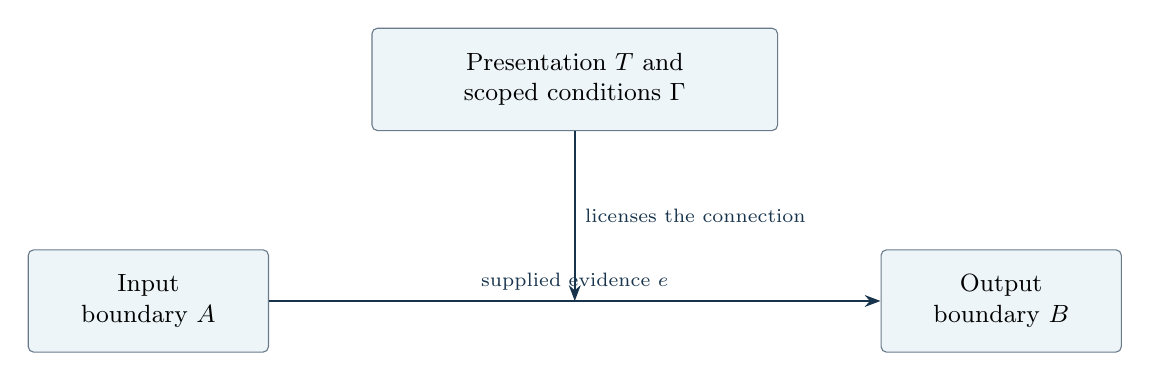
\begin{tikzpicture}
  \node[wide] (conditions) {Presentation $T$ and scoped conditions $\Gamma$};
  \node[smallbox,below left=15mm and 13mm of conditions] (a) {Input\\boundary $A$};
  \node[smallbox,below right=15mm and 13mm of conditions] (b) {Output\\boundary $B$};
  \draw[arr] (a) -- node[hint,above]{supplied evidence $e$} (b);
  \draw[arr] (conditions) -- node[hint,right]{licenses the connection} ($(a)!0.5!(b)$);
\end{tikzpicture}
\end{center}
\diagramcaption{A boundary states what must fit. The selected theory determines
whether evidence is reusable, whether an input must be consumed, and which
conversions are admissible.}

This perspective is continuous with the categorical treatment of proofs and
programs as composable processes~\cite{RosettaStone}, and with rewriting
logic's treatment of computation by proof terms~\cite{RewritingLogic}.
Variable binding requires its own substitution algebra, including weakening,
capture avoidance and metasubstitution~\cite{SecondOrderMetatheory}. These
ingredients explain how a small checker can serve many presentations without
choosing one object logic as their common meaning.

There are distinct categorical levels here. A rule with several premises is
naturally a generator of a multicategory; substitution composes proofs into
its premise slots. A sequence of unary rewrites instead gives paths in a
free category. Exchange, contraction and weakening require the structural
laws of the selected calculus. The category of checking machines describes
realizations of these proof structures, with operational observations and
costs. It is not the proof category itself. This agrees with the nLab's
accounts of deductive systems, multicategories and syntactic
categories~\cite{nLabInference}. Institutions additionally organize signatures,
models and satisfaction under change of notation; they do not by themselves
provide an executable certificate checker.

Storage navigation is a further realization level. A cursor, stack, stream,
tree focus or dependency schedule may organize the same proof evidence.
None is a primitive of every proof calculus. A focused position can be an
observation of a machine---an account of what it is currently attending
to---but a comparison must state whether it preserves that focus or hides
it. Forgetting navigation need not forget the proof's premise dependencies.
The dependency direction is from source rules to checking realizations and
then to storage adapters, rather than from a particular backend to logic.
For the authored-calculus classifying category, closed source derivations
are equivalent to arrows from the empty premise context to a singleton goal;
the two executable maps preserve the actual proof term. VibeITP and Metamath
connect their source judgments at this level, before choosing graph replay
or retained source-address checking.

\subsection{Local evidence, exact checking and coverage}

For one admitted effective presentation, let
$\mathsf{Cert}_T(\Gamma;A,B)$ be the supplied certificate data and let
$\mathsf{Valid}_T(\Gamma;A,e,B)$ be the independent validity judgment. The
local checker earns
\[
 \mathsf{check}_T(\Gamma,A,e,B)=\mathsf{true}
 \quad\Longleftrightarrow\quad
 \mathsf{Valid}_T(\Gamma;A,e,B).
\]
The separate coverage theorem relates this judgment to the intended source
relation:
\[
 A\mathrel{\mathsf{Step}_{T,\Gamma}}B
 \quad\Longleftrightarrow\quad
 \exists e.\;\mathsf{Valid}_T(\Gamma;A,e,B).
\]
The first theorem qualifies the submitted evidence. The second establishes
which source steps have a representation in that evidence language. Neither
asserts that a search procedure will find the evidence within a given budget.
Existential coverage alone also supplies no polynomial-time certificate
translator.

For an ordinary calculus with implication elimination, a local rule is
\[
 \frac{T;\Gamma\vdash p:A\qquad T;\Gamma\vdash q:A\Rightarrow B}
      {T;\Gamma\vdash\mathsf{mp}(p,q):B}.
\]
Its checker resolves the two premise citations, checks the rule instance and
compares the claimed conclusion. A resource-sensitive rule instead states how
its inputs are split or shared. Local computation can instantiate a rule;
evidence must still establish its side conditions. A negative premise such as
``no equation applies'' requires a checked exhaustion argument or a justified
index certificate.

Declaration identity belongs to this boundary. Content addressing can locate
a rule, while exact comparison or stated digest assumptions establish which
rule was found. A repeated declaration can have several occurrences despite
identical content. Certificate references must retain the occurrences required
by the observer. The host additionally identifies the theory it intended to
authorize: a valid proof under a packet's supplied theory does not identify
that theory with an externally requested one.

\subsection{Proof terms, slots and retained ambiguity}

A proof term records enough information to reconstruct the licensed use.
For an authored rewrite this can be a rule occurrence, a typed site, matching
choices, premise references and equation evidence. Deterministic fields can be
computed during replay. The current \name{GeneralRewriteRecipeExpansion}
distinguishes a compact invocation from its expanded firing receipt and proves
sound expansion and reconstruction of valid expanded firings.

Consider a two-input rule $r:(A,A)\to B$ and evidence $p,q$ of $A$.
The terms $r(p,q)$ and $r(q,p)$ record different slot assignments. Their
conclusions may coincide; identifying the derivations requires an explicit
equation or observer. Unique scoped names for slots, together with a
substitution, can encode the assignment. They do not remove choices caused
by collection matching, equations or alternative premise derivations.

Ambiguity may be useful compression. A packed proof structure can retain a
family of alternatives, just as a packed parse forest retains multiple parses.
Its boundary must say whether it certifies one selected derivation, all
represented derivations, or a complete collection of derivation occurrences.
Finding one valid branch licenses an existential claim. Certifying every
represented branch requires their local validity; claiming that the family
contains every source answer additionally requires coverage and multiplicity
laws. Backend traversal order grants none of those permissions.

The following quantities are distinct:
\[
 \text{stored nodes},\qquad \text{reference uses},\qquad
 \text{derivations distinguished by the selected observer}.
\]
A shared node can have many uses. Two positional replay choices can yield the
same firing observation, while two identical declaration copies can generate
distinct answer occurrences. The quotient must name what it forgets and prove
that the remaining consumer descends through it.

Sharing can change certificate size exponentially. A fixed example in
\name{ProofSharingBounds} has an axiom $q_0$ and the rules
$q_n,q_n\vdash q_{n+1}$. Every accepted proof tree of $q_n$ contains exactly
$2^{n+1}-1$ nodes. A chronological DAG instead stores $n+1$ nodes and two
references at each nonbase node. Its checked input size is at most
$4(n+1)^2$ even with unary rule and reference indices. The resulting theorem
excludes every polynomial-size translation from this calculus's DAGs to its
trees. This is a lower bound for the target representation, rather than a
claim about the behavior of one unfolding algorithm. It does not separate
Frege from extended Frege.

Textual parsing is another boundary. A structural certificate reader is not
the lexer and grammar of its source language. Source ambiguity must survive
in the packed parse result until an explicit policy selects, ranks or rejects
it. Binding lowering then preserves the selected scopes. The portable
presentation roundtrip supplies a proved textual surface for its supported
document schema; it does not identify every upstream module grammar with that
surface.

\subsection{The algebra of checked composition}

Five operations expose the common algebra:

\begin{tabularx}{\linewidth}{@{}p{25mm}XX@{}}
\toprule
Operation & Evidence being composed & Required law \\
\midrule
Sequence & $A\xrightarrow{p}B\xrightarrow{q}C$ & Exact joining boundary. \\
Hole filling & Premise outputs into an open derivation & Substitution respects scope and the selected structural rules. \\
Context & A local rewrite inside $C[-]$ & The context is licensed and replacement preserves its typing and binding interface. \\
Sharing & Several references to stored evidence & Every reference use remains justified and counted where required. \\
Parallel & Two orders of independent actions & Checked residual edges close the selected square. \\
\bottomrule
\end{tabularx}

\begin{center}
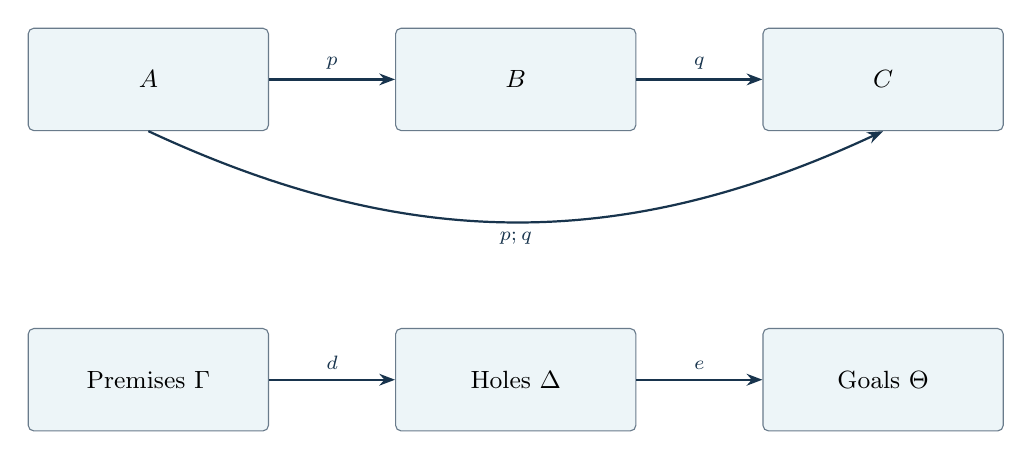
\begin{tikzpicture}
  \node[smallbox] (a) {$A$};
  \node[smallbox,right=16mm of a] (b) {$B$};
  \node[smallbox,right=16mm of b] (c) {$C$};
  \draw[arr] (a) -- node[hint,above]{$p$} (b);
  \draw[arr] (b) -- node[hint,above]{$q$} (c);
  \draw[arr] (a.south) to[bend right=25] node[hint,below]{$p;q$} (c.south);
  \node[smallbox,below=25mm of a] (g) {Premises $\Gamma$};
  \node[smallbox,right=16mm of g] (d) {Holes $\Delta$};
  \node[smallbox,right=16mm of d] (h) {Goals $\Theta$};
  \draw[arr] (g) -- node[hint,above]{$d$} (d);
  \draw[arr] (d) -- node[hint,above]{$e$} (h);
\end{tikzpicture}
\end{center}
\diagramcaption{Temporal composition and premise substitution are distinct
constructions. A particular checker realization relates them by adequacy.}

The common executable law is
\[
 \mathsf{replay}(s,p\mathbin{+\!+}q)
 =\mathsf{replay}(s,p)\mathbin{\gg\!=}
       (\lambda t.\,\mathsf{replay}(t,q)).
\]
It holds for success and refusal in
\name{DerivationGraph.replayFrom_append_eq}; the authored rewrite instance is
\name{GeneralRewriteRecipeComposition.Trace.replay_append}. Its categorical
readout is composition of \emph{partial state transformations}. A bare Boolean
verdict forgets the intermediate state needed for composition. On successful
paths, identity and concatenation give a category of checked executions.

Open derivations have another category:
\name{CertificateGSLTClassifyingCategory} takes premise contexts as objects
and vectors of open derivations as morphisms. Composition substitutes those
vectors into premise holes. Its existing Cartesian structure licenses reuse
and discard. A multi-input or linear presentation needs its corresponding
multicategorical or monoidal structure; these structural permissions are not
consequences of sequencing alone.

The authored checker already realizes the other three operations.
\name{GeneralRewriteRecipeContext} transports local receipts through admitted
typed contexts, including binders.
\name{GeneralRewriteRecipeDAG} admits local recipes and reuses the existing
shared-certificate checker for references and joins.
\name{GeneralRewriteRecipeParallel} checks four original residual firings,
independent addresses, stable site labels and literal endpoint closure; the
accepted square constructs an existing Mazurkiewicz swap. It does not infer
the missing residuals from two disjoint sites. Changed provider worlds or
observable effects require further independence evidence.

\newpage
\subsection{Checking whether another machine was stepped correctly}

Let $M$ have states $S$ and an independently stated transition relation
$s\mathrel{\longrightarrow_M}t$. Suppose local certificates $c$ have earned
the exactness and coverage contracts above. A submitted finite execution is
\[
 s_0\xrightarrow{c_1}s_1\xrightarrow{c_2}\cdots
       \xrightarrow{c_n}s_n.
\]
The checking machine threads the actual state $s_i$ and validates $c_{i+1}$
against the proposed $s_{i+1}$. Induction on the submitted sequence proves
that acceptance is equivalent to validity of all its local certificates.
Coverage then represents every finite $M$-execution. The induction uses the
actual intermediate state, so scope, heap, continuation and world components
cannot be reset between steps.

A checked instruction log is evidence of machine execution; a source evaluation
derivation supplies evidence for the source judgment. Adequacy relates their
claims. One possible result, completed evaluation and a complete result multiset
are different judgments: the latter two require the corresponding terminal or
exhaustive-branching evidence, including duplicate occurrences and pending work.

\begin{center}
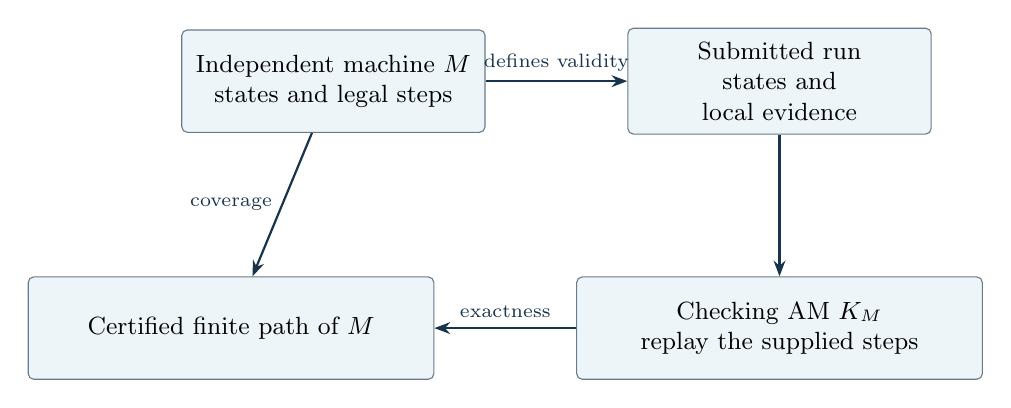
\begin{tikzpicture}
  \node[box] (spec) {Independent machine $M$\\states and legal steps};
  \node[box,right=18mm of spec] (cert) {Submitted run\\states and\\local evidence};
  \node[wide,below=18mm of cert] (checker) {Checking AM $K_M$\\replay the supplied steps};
  \node[wide,left=18mm of checker] (path) {Certified finite path of $M$};
  \draw[arr] (spec) -- node[hint,above]{defines validity} (cert);
  \draw[arr] (cert) -- (checker);
  \draw[arr] (checker) -- node[hint,above]{exactness} (path);
  \draw[arr] (spec) -- node[hint,left]{coverage} (path);
\end{tikzpicture}
\end{center}
\diagramcaption{The checked machine and its checking machine are separate
roles. A machine can play either role once the relevant evidence interface is
constructed. An empty path alone proves neither program formation nor loading
validity.}

This applies to proof-kernel instructions as readily as to CAM instructions,
rho communications or ISA transitions, when their local certificate contracts
are available. The authored GSLT implementation supplies one concrete route:
\name{GeneralRewriteRecipe.check_exact} checks its independent receipt
judgment, and \name{exists_checked_iff_step} covers the original
equation-saturated step relation. Composed recipes reach the existing finite
may-reachability native types. That modal readout establishes the witnessed
finite path; exhaustive search, termination and physical execution cost have
their own obligations.

Checking a run of $K_M$ is another instance of the same pattern. Such reflection
requires an encoding of $K_M$ and adequacy of its transition certificates.
Encoding its states as numbers or graphs preserves only the distinctions
proved for that encoding. It does not turn a certificate about a checker's run
into unconditional soundness of every theory that checker might load.

\subsection{Reconstruction, elaboration and reproducible hints}

A partial reconstructor $r$ can process output from an external prover,
tactic or repair procedure. With destination checker $c$, publication is
\[
 \mathsf{reconstruct}_{c,r}(A,o)=
 r(A,o)\mathbin{\gg\!=}
  \bigl(\lambda p.\;\mathsf{if}\ c(A,p)\ \mathsf{then}\ \mathsf{some}(p)
      \ \mathsf{else}\ \mathsf{none}\bigr).
\]
It returns $p$ exactly when $r$ returned $p$ and $c$ accepted it. No soundness
of the producer is assumed. Producer failure and checker refusal both publish
nothing; the submitted-output coverage theorem states exactly which accepted
certificates the producer can return. Composing two such stages retains both
checking boundaries. This is a general reconstruction interface, not a
completed translation of an arbitrary ATP proof format.

An elaboration has another obligation: an accepted source certificate must
produce accepted destination evidence. Existing local elaborations compose
and lift to articles. Polynomial output size, actual translation time and
logical soundness are separate properties. An output-size bound yields a
size simulation; it does not manufacture an executed polynomial-time
translator. A model interpretation likewise supplies no resource bound.

For reproducible checking, fix a deterministic strategy $f:S\to S$ and an
explicit observation $v:S\to V$ with decidable equality on $V$. A checkpoint
$(k_i,z_i)$ requests $k_i$ strategy ticks followed by the comparison
$v(f^{k_i}(s_i))=z_i$. The checker continues from its \emph{computed} internal
state, never from a replacement state supplied by the certificate. On success,
\[
 s_{\mathrm{final}}=f^{\sum_i k_i}(s_0),\qquad
 \mathsf{tickCalls}=\sum_i k_i.
\]
This remains true when $v$ forgets private theory, ownership or environment
data. A wrong checkpoint refuses at that boundary, retaining the work count
of the attempted gap. Checkpoint sequences compose from the actual residual.

Fuel alone records the budget; checkpoints additionally cross-check selected
residual observations; a full trace records one observation per tick. The
formal materializer produces exactly $n$ trace entries from budget $n$.
All three replay the specified computation: checkpoints alone do not make
the intervening computation cheaper. Tick calls, observation comparisons,
stored observation sizes and native instructions require distinct accounts.
Implementation heartbeats are not interchangeable with these strategy ticks.

The Lean4Lean instance uses its existing finite-catalog beta/delta/head
algorithm. Its checkpoints include the expression and a terminal flag.
Acceptance proves a path in the independent head-event relation and an
endpoint with no remaining head event. Completeness is relative to this
strategy reaching a common head-normal form. The raw self-application term
$\Omega$ remains pending at every budget, yet every submitted finite
normalization certificate is refused. This instance neither requires nor
asserts termination of arbitrary Lean conversion, and it is not the complete
Lean type-checking kernel.

The algorithmic and ideal judgments must also be distinguished. Lean4Lean
implements a particular checking algorithm and separately studies the
declarative type theory; verification of its implementation is partial
work~\cite{Lean4Lean}. An exact contract for an algorithmic judgment does not
decide every ideal equality. If a family of budgets enumerates exactly the
same algorithmic successes, an ideal equality absent from that set remains
absent at every budget. This is a theorem about the acceptance boundary,
independent of implementation heartbeats.

Within a fixed formed-expression fibre, checked comparisons may instead be
leaves of explicit reflexivity, symmetry and transitivity recipes. The
checker computes their endpoints and refuses a mismatched intermediate
join. It has exact authority for the equivalence closure
$\operatorname{EqvGen}(R_{\mathrm{alg}})$ of the independent leaf relation.
Soundness into ideal equality follows from a sound leaf interpretation.
Completeness for ideal equality additionally requires the generation theorem
$R_{\mathrm{ideal}}\subseteq\operatorname{EqvGen}(R_{\mathrm{alg}})$; it is
not supplied by fuel or by categorical composition alone. On raw syntax,
ideal typed equality need not be reflexive: formation remains an explicit
obligation before entering this fibre. The finite nontransitive control in
the library illustrates this distinction without claiming to be a
counterexample from Lean's full conversion implementation.

Lean4Less gives a concrete reason to separate these routes: it replaces
selected implicit proof-irrelevance and K-like conversions with explicit
equality proofs and transports, then checks the output with those conversion
features disabled~\cite{Lean4Less}. This is an elaboration between equality
profiles, with separate declaration, universe and resource obligations.
Destination rechecking can validate a proposed output even when the producer
is partial; neither a total translator nor a polynomial size bound follows
from that check. The present boundary theorems do not complete either
external system's metatheory.

The practical propositional connection reuses Lean's verified LRAT checker
for RUP, RAT and deletion actions~\cite{LRAT}. Its adapter preserves native
clause satisfaction pointwise, including repeated literals and clauses.
Accepted refutations imply an empty-clause derivation in the independently
complete resolution calculus. That implication supplies no polynomial
LRAT-to-resolution compiler. The public checker may stop at a successful
empty-clause action, so its verdict does not validate an unused action suffix.

Finite intuitionistic and classical Hilbert certificates are checked directly
by their formula instances and ordered premises. The existing standard
Hilbert calculi in Foundation supply the independent source judgments;
soundness and tree/DAG coverage are proved against them. The classical
profile admits excluded middle, while the intuitionistic profile refuses
that rule. A computable elaborator now returns terms in the existing
\code{PropDeriv} family from accepted certificates, using the supplied
children and a computed finite lookup rather than choosing an existential
proof. The retained-term interface publishes a term exactly when the native
checker accepts the requested formula.

Intuitionistic non-theorems have a complementary finite certificate: a
partial-order table, a persistent atomic valuation, and a refuting world.
The checker validates those tables and computes the Kripke semantics of the
formula. Soundness follows through the independent source semantics;
Foundation's finite-model completeness supplies a finite data certificate
for every non-theorem. A two-world control refutes excluded middle, while
malformed orders, nonpersistent valuations and out-of-range worlds refuse.

Proof and countermodel certificates are countably encoded as finite data.
Enumerating those codes until one validates gives an executable terminating
decision procedure for the original intuitionistic theorem judgment.
Termination uses the two coverage theorems, not an ideal decision oracle.
Submitted proofs or countermodels can be checked first as hints; incorrect
hints are skipped and the same total search remains available. The least
successful index is bounded by the code of any supplied valid certificate.
This exhaustive construction proves decidability. Its search order has no
practical complexity claim and is separate from the native replay kernel.

The classical extension checker adds literal hypotheses
$p_i\leftrightarrow A_i$ with fresh names. It refuses a name appearing in
the final claim, any earlier declaration, or its own right-hand side.
Definitions are hypotheses, never additional substitution-closed axiom
schemes. A valuation of the old vocabulary extends in declaration order to
satisfy every definition while preserving the claim. Consequently the
extension checker has exactly the ordinary classical theorems. Native tree
and shared-DAG coverage are proved. The direct Frege-DAG embedding retains
all formulas, parent references and node counts, and has the same replay
verdict; no tree expansion is involved.

Literal elimination of definitions has a separately measured cost. The
admitted chain $p_{i+1}\leftrightarrow(p_i\wedge p_i)$ has encoded size at
most $5(n+1)(n+2)$, including unary name costs and the final reference.
The specified last-definition-first unfolding algorithm returns a formula
with exactly $2^{n+1}-1$ nodes. This bounds that literal materialization
policy. It is not a lower bound on every equivalent formula, nor a
separation between unrestricted Frege and extended Frege. An executed
Cook--Reckhow polynomial bound remains a further obligation.

\subsection{Retained checking, suspension and evidence release}

A checking configuration retains what its remaining work needs:
\[
 K=(T,\Gamma,\mathsf{cache},\mathsf{boundary},
       \mathsf{residual},\mathsf{obligations},\mathsf{status}).
\]
The concrete representation may use references and shared tables. World
revisions, provenance and consuming rights enter those components where the
selected calculus requires them. Accepting a local instruction extends the
checked prefix; final acceptance additionally requires the requested root and
all obligations required for that claim.

As one storage realization, the authored-calculus cursor instantiates this
retained machine directly.
Its completed successful runs are exactly licensed runs of the original
source rows, including unused rows in the submitted schedule. VibeITP's
instance preserves its independently specified static theorem judgment and
auxiliary term-operation judgments. Metamath's projected snapshot connects
common graph acceptance to successful original normal-label execution under
its projection and empty-stack hypotheses. Neither connection replaces
parser provenance or native storage refinement.

Portable calculus modules retain both the complete term-language base and
the proof-calculus layer. The verified text reader, followed by the original
calculus validator, recovers the exact selected package. Malformed text,
another layer schema and failed validation cannot select that package.
This is the portable module data surface, separate from the upstream
theory-builder grammar. Reading declarations grants no theorem authority.

\begin{center}
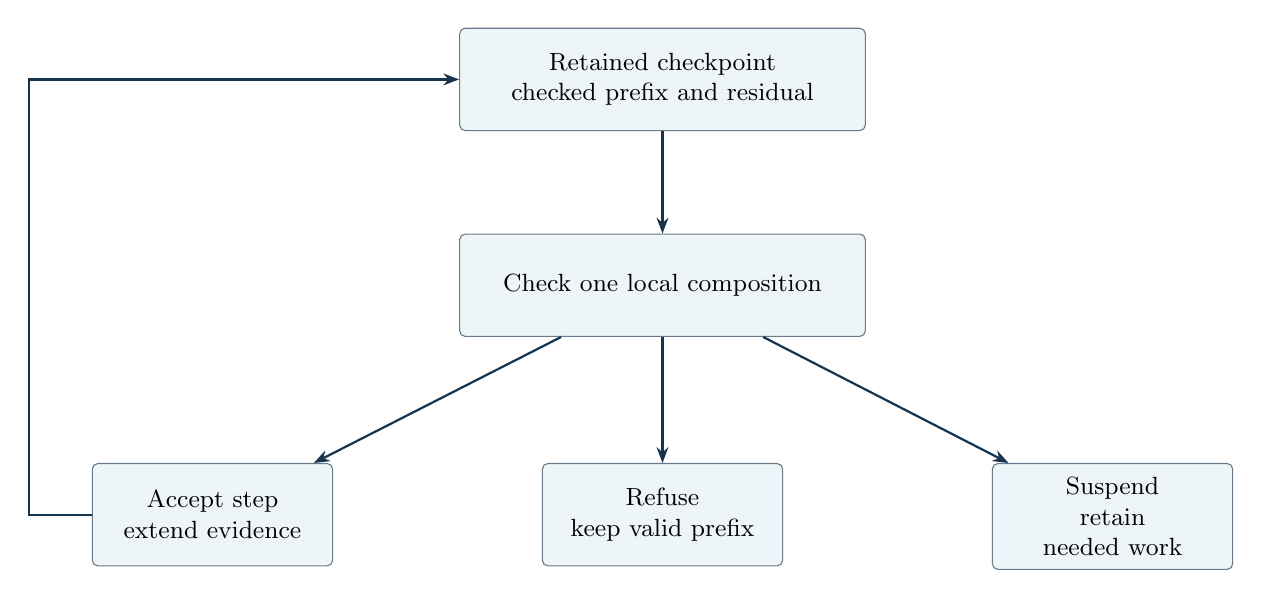
\begin{tikzpicture}
  \node[wide] (saved) {Retained checkpoint\\checked prefix and residual};
  \node[wide,below=13mm of saved] (step) {Check one local composition};
  \node[smallbox,below left=16mm and 16mm of step] (accept) {Accept step\\extend evidence};
  \node[smallbox,below=16mm of step] (refuse) {Refuse\\keep valid prefix};
  \node[smallbox,below right=16mm and 16mm of step] (wait) {Suspend\\retain needed work};
  \draw[arr] (saved) -- (step);
  \draw[arr] (step) -- (accept);
  \draw[arr] (step) -- (refuse);
  \draw[arr] (step) -- (wait);
  \draw[arr] (accept.west) -- ++(-8mm,0) |- (saved.west);
\end{tikzpicture}
\end{center}
\diagramcaption{Missing evidence, exhausted checking budget and an unanswered
external request are different suspension reasons. Refusing the supplied
certificate establishes neither falsity nor unreachability of its claim.}

The retained law is
\[
 \mathsf{advance}(m+n,K)
   =\mathsf{advance}(n,\mathsf{advance}(m,K)).
\]
It compares complete checkpoints. MM0 assertion execution and the HOL Light
source receiver already instantiate \name{ResumableTrajectory}. For MM0,
the command tail and unification continuation remain live; final assertion
validation is a separate observer. For HOL Light, \name{EventWork} retains
the accepted theory/proof state, remaining JSON events and refusal status.
A refused event stays at the residual's head. Accepted receipt prefixes grow
without replay, and two separately identified reflexivity events with the same
conclusion remain two occurrences. The budget counts source events, whose
local costs need not coincide.

The authored recipe DAG and equation-application DAG now have retained
workers over their original nodes and checkers. Each checks one submitted row
per transition, retaining the last accepted table and the entire refused
suffix. Their completed verdicts are exactly the existing certificate
verdicts, and their actual runs finish within the number of rows plus one
finishing transition. The rho tree worker similarly inspects one original
inference occurrence per transition, with exact recursive-checker agreement
and a bound of the tree's node count plus one. Endpoint formation remains an
additional rho request-boundary check. These bounds count calls of the local
worker; they do not price every internal substitution or equality operation.
For authored GSLTs, existence of an actual terminated checker run with an
accepted root is equivalent to inhabiting the existing reaching native type
for an equation-respecting target predicate. The native-type readout therefore
comes from the original finite rewriting semantics, rather than a command
layer with an unspecified local step.

All these workers are objects of the existing machine category at their own
observation interfaces. The MM0 instance keeps its command and unification
microsteps, the HOL Light instance keeps its registered source-event receiver,
and the Lean4Lean head-profile instance keeps its actual head strategy.
Choosing a common observation interface and proving a bounded stage between
two objects are additional obligations. Object construction alone supplies
no translation of one native logic into another.

Retention is governed by future use, not by a requirement to keep every detail
forever. For ordinary value readouts $d$ in a declared consumer family $\mathcal D$,
replacing a detailed record by $q(x)$ is licensed when
\[
       \forall d\in\mathcal D\;\exists\bar d.\qquad d=\bar d\circ q.
\]
Dependent evidence additionally needs coherent family and section descent.
An outstanding obligation must be discharged or transferred under its own
authority contract. Once a recipient owns the needed evidence and every
remaining local consumer factors through the retained summary, the sender
may release detail that no longer serves those obligations. A newly admitted
consumer cannot recover erased distinctions merely by requesting them.

\subsection{A category of machines and realization stages}

For fixed event, verdict and request types $(E,V,Q)$, the existing
\name{ObservedMachine} bundles an actual state carrier $S$ and productive
stepper $M:S\to\mathsf{Option}(\mathsf{Transition}(S,E,V,Q))$.
Its morphisms are the existing \name{Stage} contracts: a relation between
source and target states, a forward cost-bounded simulation and completion
reflection. Identity uses the equality relation at bound one. For stages
$(R,c)$ and $(S,d)$, composition has
\[
 (S\circ R)(x,z)\ \Longleftrightarrow\
       \exists y.\;R(x,y)\wedge S(y,z),
 \qquad \mathsf{cost}=dc.
\]
\name{Stage.refl_comp}, \name{Stage.comp_refl} and
\name{Stage.comp_assoc} supply the category laws. The
\name{ObservedMachine.relabelFunctor} maps a common observation interface
to another while retaining the underlying state carriers. Noninjective label
maps can forget distinctions; each dependent consumer needs its own descent
law before using that coarser view.

\begin{center}
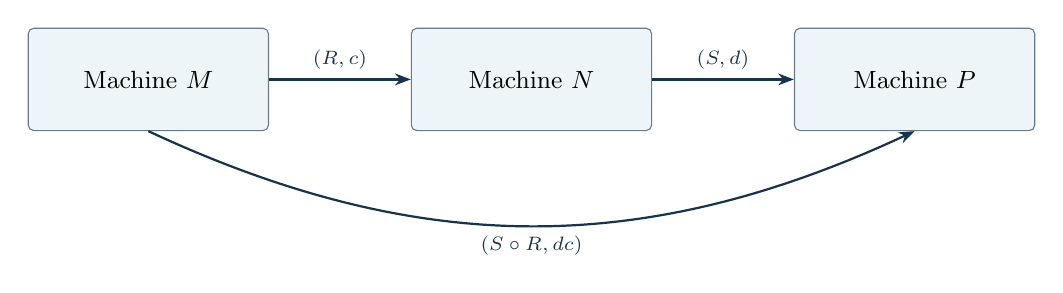
\begin{tikzpicture}
  \node[smallbox] (m) {Machine $M$};
  \node[smallbox,right=18mm of m] (n) {Machine $N$};
  \node[smallbox,right=18mm of n] (p) {Machine $P$};
  \draw[arr] (m) -- node[hint,above]{$(R,c)$} (n);
  \draw[arr] (n) -- node[hint,above]{$(S,d)$} (p);
  \draw[arr] (m.south) to[bend right=25]
    node[hint,below]{$(S\circ R,dc)$} (p.south);
\end{tikzpicture}
\end{center}
\diagramcaption{Composition retains the declared relational contract and
resource bound. It neither selects a compiler implementation nor identifies
all intermediate execution witnesses.}

The controls make the distinction concrete: two stages with bound three
require composite bound nine; the proposed sum six fails. A checker/interpreter
round trip preserves its final observation but differs from the identity
stage because its retained cost bound is three. The bound is a proved account
for the chosen machine transitions, not a measurement of native time.
The present \name{Stage} contract reflects completion; preserving stuckness
versus silent divergence requires further endpoint laws. An existing negative
control relates a stuck source to a spinning target under the weaker contract.
The extra \name{MatchesStuck} obligation excludes that case.

There is also a general finite-trace relational envelope. Fix observable
words $w$, with internal steps erased by a declared observer. For branching
machines, take relations $R$ satisfying
\[
 R(s,u)\ \wedge\ s\overset{w}{\Longrightarrow}_M t
 \quad\Longrightarrow\quad
 \exists v.\;u\overset{w}{\Longrightarrow}_N v\ \wedge\ R(t,v).
\]
Equality is an identity relation. Relational composition preserves this law:
choose the intermediate related state, match the source path in the middle
machine, then match that middle path in the final machine. Relational unit
and associativity laws therefore give a category at this extensional contract
level. This mathematical schema states a finite may-preservation profile;
backward, divergence, probability and resource obligations enrich it separately.
The concrete kernel-checked category above currently uses deterministic
steppers, whose schedules may realize branching source calculi only through
their own adequacy theorem.

Vacuous relations are not executable realizations. Loading must relate every
admitted source entry to an actual target entry; representation, request/reply
and authority laws complete the applicable contract. Furthermore, forgetting
the middle state can erase information required by a dependent result.
\name{DependentComposition.Path} retains that state as data; its descent
theorems identify when transport is independent of the chosen middle witness.
Thus a category of endpoint contracts and a richer account of executions can
coexist, with information release justified at the selected boundary.

\subsection{Fibres, crossings and a machine of machines}

The functional GSLT construction is already literal category theory.
\name{OperationalTranslation} preserves equations and source steps;
\name{CoveredTranslation} additionally covers target steps at image states.
The functor \name{executionIndex} sends each operational theory $L$ to its
category of finite execution paths. Its Grothendieck construction has objects
$(L,s)$ and arrows
\[
 (L,s)\longrightarrow(K,t)
 \quad=\quad
 \bigl(f:L\to K,\;p:F(f)(s)\longrightarrow t\bigr).
\]
For $f:L\to K$, $g:K\to H$ and compatible paths $p,q$, the composite is
$(g\circ f,F(g)(p);q)$. Identity and associativity follow from the base and
fibre laws and the functor laws. This is a constructed total category for
functional operational transport. Its underlying proposition-valued steps do
not distinguish two rule occurrences with identical endpoints; receipts or
labelled edges retain such distinctions when required.

\begin{center}
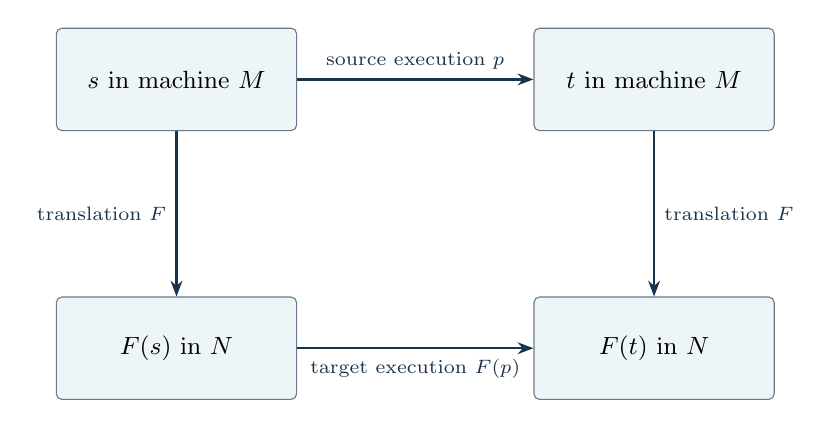
\begin{tikzpicture}
  \node[smallbox] (s) {$s$ in machine $M$};
  \node[smallbox,right=30mm of s] (t) {$t$ in machine $M$};
  \node[smallbox,below=21mm of s] (fs) {$F(s)$ in $N$};
  \node[smallbox,right=30mm of fs] (ft) {$F(t)$ in $N$};
  \draw[arr] (s) -- node[hint,above]{source execution $p$} (t);
  \draw[arr] (s) -- node[hint,left]{translation $F$} (fs);
  \draw[arr] (t) -- node[hint,right]{translation $F$} (ft);
  \draw[arr] (fs) -- node[hint,below]{target execution $F(p)$} (ft);
\end{tikzpicture}
\end{center}
\diagramcaption{A functional path map supplies a commuting square. Relational
block simulations instead retain related endpoints and their actual matching
paths; their coherence is an additional construction.}

The executable \name{GSLTILNativeKernel} separates stepping inside a fibre
from crossing an explicit route. The installed \name{GSLTILAuthoredFibre}
uses the actual authored rewrite checker and its source-coverage theorem.
It currently installs no translation routes. Its \code{at}/\code{via}
dispatcher can host locally justified routes, but does not manufacture their
interpretations, resource transport or conservativity.

A broader web can retain relational simulations and comparison cells instead
of forcing all crossings into state functions. Horizontal paths then concern
executions within a regional machine; vertical comparisons relate configurations
of different machines; a cell supplies the matched execution evidence. These
cells need their own composition and coherence laws. Substitution, logical
interpretation, world update and authority transport retain different
preservation contracts even when they occur in one diagram. This is the
remaining generalization, not an implication of the Grothendieck name.

\subsection{Regional kernels, semantic faces and open-ended reflection}

The checking machine has an operational run; its accepted evidence inhabits
an intensional derivation judgment; model interpretation supplies an
extensional face. These comparisons form the computational trinity around the
checker. Logical soundness goes from derivations to validity in the selected
models. Logical completeness, where established for the particular fragment,
goes in the other direction. Coverage of certificate representations is
instead a comparison with derivations. These three claims have different
hypotheses and do not identify the faces.

MM0 makes the distinction between its readable specification and binary proof
program explicit~\cite{MM0}. Its verifier computes with stacks, hypotheses,
terms and binder data, and declaration agreement binds that computation to
the intended specification and preceding environment. HOL Light supplies
kernel-authorized inference through the LCF interface~\cite{HOLLight}; its
theorem cache and receipt graph have a separate retained execution account.
Megalodon checks typed proof objects with normalization and delta expansion
under its selected environment. OpenTheory articles give a textual proof
stack machine~\cite{OpenTheoryArticle}; CakeML includes a verified article
checker and Candle's HOL Light implementation~\cite{CakeMLProofMachines}.
These are regional realizations, with distinct logical commitments and
checking disciplines.

Lambdapi and HOL Light exercise different binder obligations. Lambdapi's
restricted higher-order rewrite patterns test scoped matching under
binders~\cite{LambdapiRules}. HOL Light's primitive replay tests term/type
instantiation and theorem construction. Real HE and PeTTa evaluation kernels
must likewise use their own independent judgments: a certified rewrite at one
atom's root does not establish the dialect's nested evaluation, quoted/raw
arguments, complete result multiplicity or retained effects.

Structural compilation of an admitted profile and checking a finite execution
are complementary hosting routes. Partial recursive checkers admit finite
bounded-evaluation witnesses~\cite{MathlibPartrecCode}; actual hosting still
requires the source encoding, target certificate construction and checker
adequacy. A p-simulation further requires a polynomial-time proof translator
under declared encodings, hence polynomial output size. A short operation
name does not make a large substitution or conversion cheap. Shared-node
size, expanded uses and executed work require separate accounts.

Small primitive inventories, weak logical assumptions and cheap checking are
different objectives. The existing inference-basis theory supplies
inclusion-minimal generating subsets for a finite inventory, including
incomparable minima with no least generating basis. It supplies neither an
efficient minimizer nor a universal least kernel. The common interface is
licensed composition; individual presentations choose their generating rules
and prove their interpretation.

An interactive prover additionally retains open goals, scoped metavariables,
substitutions and delayed constraints. Its search may diverge or remain
incomplete even when each closed certificate is finitely checkable. Reflection
makes these presentations and checking processes available as data. Goertzel's
reflective metagraph account motivates this internal availability of rules and
their transformations~\cite{ReflectiveMetagraph}. Weinbaum's open-ended
intelligence motivates admitting new vocabularies and observers rather than
requiring a final fixed inventory~\cite{WeinbaumThesis}. The architectural
proposal is to combine that openness with explicit crossings: changing a
theory exposes new commitments, replacing a machine preserves the declared
observations, and neither silently changes what an earlier certificate proved.

\sources{\name{Mettapedia/Logic/DerivationGraph.lean},
\name{Mettapedia/GSLT/LanguageDef/CertificateGSLTClassifyingCategory.lean},
\name{Mettapedia/OSLF/MeTTaIL/GeneralRewriteRecipe.lean},
\name{Mettapedia/OSLF/MeTTaIL/GeneralRewriteRecipeExpansion.lean},
\name{Mettapedia/OSLF/MeTTaIL/GeneralRewriteRecipeComposition.lean},
\name{Mettapedia/OSLF/MeTTaIL/GeneralRewriteRecipeContext.lean},
\name{Mettapedia/OSLF/MeTTaIL/GeneralRewriteRecipeDAG.lean},
\name{Mettapedia/OSLF/MeTTaIL/GeneralRewriteRecipeExecution.lean},
\name{Mettapedia/OSLF/MeTTaIL/GeneralRewriteRecipeParallel.lean},
\name{Mettapedia/GSLT/Distinction/SimulationComposition.lean},
\name{Mettapedia/GSLT/Distinction/SimulationCompositionControls.lean},
\name{Mettapedia/GSLT/Distinction/DependentComposition.lean},
\name{Mettapedia/GSLT/Core/OperationalPathFibration.lean},
\name{Mettapedia/GSLT/LanguageDef/GSLTILAuthoredFibre.lean},
\name{Mettapedia/Languages/MM0/Formats/MMB/MachineCost.lean},
\name{Mettapedia/Languages/MM0/MeTTa/Formats/MMB/ExecutedSoundness.lean},
\name{Mettapedia/Languages/HOLLight/IncrementalExecution.lean},
\name{Mettapedia/Languages/HOLLight/KernelAtlas.lean},
\name{Mettapedia/Languages/MeTTa/EquationKernel/Execution.lean},
\name{Mettapedia/Languages/ProcessCalculi/RhoCalculus/NativeExecution.lean},
\name{Mettapedia/Languages/Lean/HintedHeadConversion.lean},
\name{Mettapedia/Languages/Lean/Lean4LessCheckerBoundary.lean},
\name{Mettapedia/Logic/EqualityRecipe.lean},
\name{Mettapedia/Computability/FuelledConversionEvidence.lean},
\name{Mettapedia/Machines/ExecutionHints.lean},
\name{Mettapedia/GSLT/LanguageDef/KernelCheckingClasses.lean},
\name{Mettapedia/GSLT/Logic/PropositionalLRAT.lean},
\name{Mettapedia/Logic/PropositionalExtension.lean},
\name{Mettapedia/Logic/IntuitionisticDecision.lean},
\name{Mettapedia/Logic/PropositionalHilbertChecking.lean},
\name{Mettapedia/Logic/ProofSharingBounds.lean},
\name{Mettapedia/Coalgebra/CoherentPrefixTower.lean},
\name{Mettapedia/Logic/InferenceBasis.lean}.}
\scope{Local authored checking, its composition operations, functional path
transport, costed stage composition, checked reconstruction and the retained
native checker instances are constructed at their stated contracts. Authored packet coverage
uses the existing admission compiler and an empty dynamic provider; textual
module parsing is a separate front end. The finite-trace
relational envelope is a mathematical schema. A complete heterogeneous
execution/certificate web, its route authentication, general relational
coherence and native physical resource bounds remain further constructions.}


\newpage
\section{Execution contracts: determinism is one dimension}
\label{sec:contracts}

A deterministic implementation can enumerate many answers, compute an entire
distribution, or simulate concurrent processes under a selected schedule.
A sampler can return exactly one answer while representing a nontrivial
probability law. These properties therefore cannot be represented by one
exclusive choice between deterministic, nondeterministic and probabilistic.

\begin{tabularx}{\linewidth}{@{}p{34mm}XX@{}}
\toprule
Dimension & Contract question & Distinguishing example \\
\midrule
Transition & At most one next state? & An ordered search driver steps
deterministically through many alternatives. \\
Cardinality & How many successful occurrences in a completed run? & Two equal
answers count twice. \\
Completion & Is any work still pending? & One answer followed by a suspended
branch is not a closed singleton. \\
Probability & What measure describes outcomes? & A fair and a biased coin
have the same finite support. \\
Concurrency & Which enabled actions may be scheduled? & Two independent
actions can commute without one global deterministic schedule. \\
Commitment & Which alternatives or effects may be discarded? & \code{once}
selects a success; it does not prove there was only one. \\
\bottomrule
\end{tabularx}

\subsection*{Cardinality belongs to a calling mode and its world}
The existing answer grades bound the number of occurrences in a completed
answer collection: zero, exactly one, zero-or-one, one-or-more, or unrestricted.
Relational choice adds occurrence counts; an exclusive conditional combines
bounds by an interval hull. Sequential binding applies a bound separately
to each reachable input occurrence with its bindings. Types, instantiation,
termination, faults and effects remain additional obligations. A declaration
of \code{det} expresses a contract; an optimization needs evidence for the
actual calling mode and relevant provider revision.

The current weighted cardinality consumer accepts a complete cut only when
it is empty or contains one returned occurrence. It preserves that occurrence's
coefficient, including zero. A cut with a pending state is refused even if
its current returned prefix has length one. The accepted result is stable
under further resumption. This is a representation theorem about an already
computed cut, not a procedure for deciding termination or safely pruning
an unfinished search. Probing for another answer can perform effects,
force otherwise unused work, or diverge.

\subsection*{What a deterministic region can improve}
The independently defined queued and direct executors already agree on
ready operands, functional primitives, worlds, ordered effects, failures and
instruction-boundary residuals. Their primitive invocation counts agree;
their modeled dispatch counts differ. This licenses eliminating that queue
within the admitted region. It establishes no native speedup and does not
yet cover arbitrary expressions, binding merges or concurrent mutation.

\sources{\name{Mettapedia/Machines/AnswerCardinality.lean},
\name{Mettapedia/Machines/DeterministicRegion.lean},
\name{Mettapedia/Machines/OccurrenceMachine.lean},
\name{Mettapedia/GSLT/Dynamics/WeightedBranchingCardinality.lean}.}

\newpage
\subsection{Probabilities, coefficients and schedules}

A coefficient is not automatically a probability. The weighted resumption
interfaces work with algebraic coefficients and preserve pending contributions
and occurrence identity. A probabilistic interpretation additionally needs
nonnegative mass and a specified normalization or subnormalization law.
An importance weight, a scheduling priority, a cost and an ownership permission
are different quantities even when they use similar algebraic notation.

\begin{center}
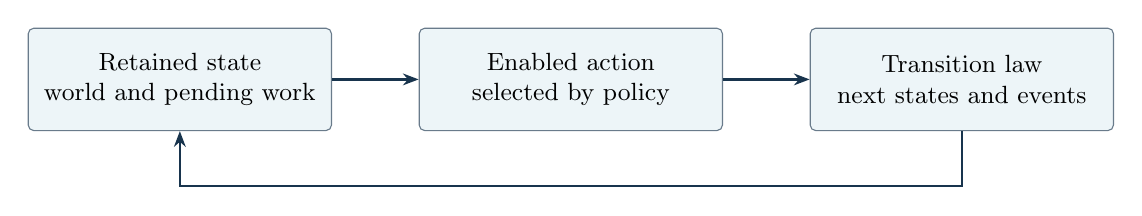
\begin{tikzpicture}
  \node[box] (state) {Retained state\\world and pending work};
  \node[box,right=11mm of state] (action) {Enabled action\\selected by policy};
  \node[box,right=11mm of action] (law) {Transition law\\next states and events};
  \draw[arr] (state) -- (action);
  \draw[arr] (action) -- (law);
  \draw[arr] (law.south) -- ++(0,-7mm) -| (state.south);
\end{tikzpicture}
\end{center}
\diagramcaption{A scheduler selects an enabled action; a probabilistic kernel
specifies its stochastic transition. Relational alternatives need not carry a
canonical probability law. A point mass recovers deterministic transition.}

Combining nondeterministic choice with probability is a semantic choice:
the available scheduler information and the order of the two effects matter.
One cannot assume that an arbitrary combination of the familiar monads has
the desired distributive laws~\cite{ProbNondet}. A machine contract should
state the admissible policies and what the observer compares: possibilities,
ordered occurrences, trace distributions, or another declared quantity.

The existing finite probabilistic systems use subdistributions and account
for missing mass as declared refusal. Their probabilistic bisimulation retains
more information than the support relation. However, the system record does
not itself prove that its kernel follows the underlying GSLT rewrite relation;
that is an operational bridge still to construct. Erasing probabilities to
possibility support cannot justify a probability-preserving implementation.
For a continuous distribution, a singleton can have probability zero without
being an impossible value; positive point mass is not a general support test.

\subsection*{Sampling, scoring and resumption}
A retained draw needs its dynamic occurrence identity and original world.
Resuming a committed draw must reuse its result. Calling a resampled suspension
creates a new occurrence; merely sharing written syntax does not establish
stochastic independence. Independence requires a law for the actual joint
execution, often conditional on captured latent variables.

Scoring generally produces an unnormalized measure. Forming a posterior
requires an evidence mass $Z$ with $0<Z<\infty$; zero or infinite evidence
needs explicit treatment. Retention must preserve committed factors and avoid
applying them again. Existing coefficient plumbing is useful here, but it
does not supply this entire probability-and-authority contract.

\scope{No production port is licensed solely by cardinality or coefficient
laws. The complete world, bindings, effect history, faults, ownership and
residual demand must travel through the same constructed correspondence.}

\sources{\name{Mettapedia/GSLT/Dynamics/WeightedResumption.lean},
\name{Mettapedia/GSLT/Dynamics/WeightedBranchingResumption.lean},
\name{Mettapedia/GSLT/Distinction/Probabilistic/System.lean},
\name{Mettapedia/GSLT/Distinction/Probabilistic/Semiring.lean},
\name{Mettapedia/ProbabilityTheory/IndependentFiniteSampling.lean}.}

\newpage
\section{Focus, zippers and typed graph holes}
\label{sec:holes}

For regular tree syntax, the derivative of a datatype describes its one-hole
contexts~\cite{Derivative}. A zipper retains a focused subtree and the
context needed to rebuild its surroundings~\cite{Zipper}. Indexed
polynomials extend this organization with context and sort information;
dissections distinguish already processed positions from remaining positions.
These are representation and navigation tools. A legal position is not by
itself permission to evaluate, force, sample or commit an effect.

\begin{center}
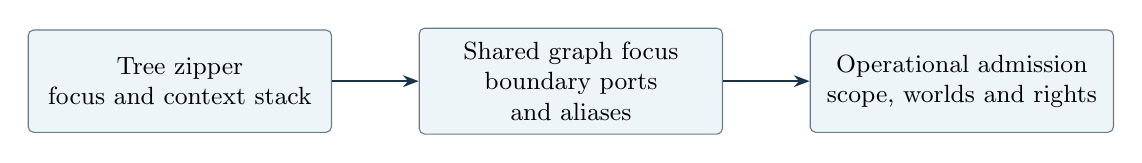
\begin{tikzpicture}
  \node[box] (tree) {Tree zipper\\focus and context stack};
  \node[box,right=11mm of tree] (graph) {Shared graph focus\\boundary ports and aliases};
  \node[box,right=11mm of graph] (rights) {Operational admission\\scope, worlds and rights};
  \draw[arr] (tree) -- (graph);
  \draw[arr] (graph) -- (rights);
\end{tikzpicture}
\end{center}

The existing PathMap zipper interface transports query membership under
iteration and store-agreement hypotheses. Concrete flat and trie instances
prove particular traversal and rebuilding laws. This is useful ZAM structure;
it is not a proof of the full native Rust machine, ordered query multiplicity,
or its world and demand semantics. A membership theorem alone cannot establish
that two equal rows produce two answer occurrences.

\subsection*{A shared hole needs an interface, not just a path}
Replacing a shared subgraph affects every alias to it. A graph hole therefore
needs the incoming and outgoing ports crossing its boundary, their scoped
types, identity and sharing requirements, and the resources or obligations
that move with them. A single tree path loses those other connections.
Cycles require the corresponding consistency and update rules. Bag or set
quotients also need occurrence identities when their physical ordering is
not canonical.

Goertzel's reflective metagraph account makes programs and rewrite rules
graph data~\cite{ReflectiveMetagraph}. Graph rewriting's preserved interface
and gluing conditions are useful guidance: a replacement must account for
the links it preserves and those it removes. This motivates a runtime contract;
it does not already provide a typed effectful graph-hole machine.

\subsection*{Different holes have different filling rules}
An unknown source fragment, a paused computation, a stochastic latent variable,
an external response and an unfulfilled proof obligation are not interchangeable.
The existing pure higher-order hole evaluator retains environments and
indeterminate operations. Its filling/resumption equivalence has a termination
condition. Its controls show that divergent call-by-value fillers and effectful
reordering can break an unrestricted equivalence. The tree multi-hole monad
also deliberately permits capture; it is not a ready-made hygienic shared-graph
interface. Filling must establish the applicable scope and execution contract.

\sources{\name{Mettapedia/GSLT/Poly/BindingSignature.lean},
\name{Mettapedia/GSLT/Poly/SortedTraversal.lean},
\name{Mettapedia/OSLF/PathMap/ZipperExecution.lean},
\name{Mettapedia/OSLF/PathMap/Trie/HuetZipper.lean},
\name{Mettapedia/OSLF/Programs/HoleEvaluation.lean},
\name{Mettapedia/OSLF/MeTTaIL/MultiHoleContext.lean},
\name{Mettapedia/GraphTheory/Representation/Metagraph.lean}.}

\newpage
\subsection{A core MAM for heterogeneous retained computations}

The strongest candidate here separates execution, dependency accounting and
reflection. They refer to the same occurrence identities, but they need not
use one physical representation. A machine can execute a compact packed
region while exposing a metagraph view on demand. Reflection need not allocate
a public syntax object for every primitive instruction.

\begin{center}
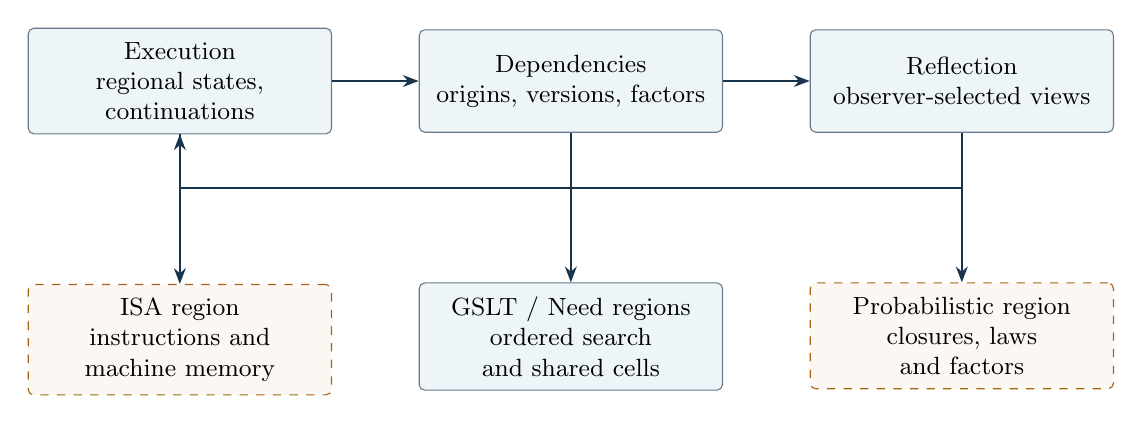
\begin{tikzpicture}
  \node[box] (execution) {Execution\\regional states, continuations};
  \node[box,right=11mm of execution] (dependency) {Dependencies\\origins, versions, factors};
  \node[box,right=11mm of dependency] (reflection) {Reflection\\observer-selected views};
  \draw[arr] (execution) -- (dependency);
  \draw[arr] (dependency) -- (reflection);
  \draw[arr] (reflection.south) -- ++(0,-7mm) -| (execution.south);
  \node[future,below=19mm of execution] (isa) {ISA region\\instructions and machine memory};
  \node[box,below=19mm of dependency] (gslt) {GSLT / Need regions\\ordered search and shared cells};
  \node[future,below=19mm of reflection] (ppl) {Probabilistic region\\closures, laws and factors};
  \draw[arr] (execution) -- (isa);
  \draw[arr] (dependency) -- (gslt);
  \draw[arr] (reflection) -- (ppl);
\end{tikzpicture}
\end{center}
\diagramcaption{Dashed regions mark unconstructed general interfaces. All regional
calls use the crossing contract; the connecting lines do not assert an ISA or
higher-order probability correspondence already exists.}

The proposed retained state includes local computations, typed open boundaries,
shared producer/use identities, ordered alternatives, world dependencies,
committed draws and factors, consumed rights, and selected observations.
Its transitions admit and focus a region, advance it, deliver a request or
reply, fill an authorized hole, validate dependencies, pause, or dispose of
cancelled obligations. Sampling and scoring come from an admitted regional
semantics. Neither graph shape nor a type annotation silently authorizes them.
Logical guests retain their own judgment systems; a common port protocol
does not make their propositions interchangeable.

Qualification would lift local correspondences through admitted graph
contexts, fillings and crossings. At publication, suspension and return,
the chosen trace observations and related residuals must survive together.
Probabilistic regions compare the resulting laws under declared scheduling
policies, or a stated coupling bound; equal possible values are insufficient.
These compatibility laws must be proved for the actual assembly. Listing
types and authority metadata does not establish them.

An ISA region would load code with an instruction-validity contract and retain
registers, memory, faults and external-service state. Its source translation
must state ABI and memory assumptions. The existing register-code machine
supplies a narrower lowering and execution connection; a proposed
\code{lts:isa} interface is not established by that result. Cesta macro
elaboration belongs to a staging phase, before the resulting C/native region.

A GSLT interpreter is a general rule-execution machine. Calling it UTM-tier
requires an encoding of universal computation and a correspondence theorem.
Even such a theorem would not preserve fairness, ordered occurrences, costs,
probability laws or ownership automatically. Those are regional contracts,
not consequences of computational universality.

\scope{This architecture is a research target assembled from existing owners.
It is not an implemented universal MAM or a claim that one representation is
optimal for every region. Its first consumer remains the actual MeTTa
source/native and owned-interaction connection.}

\sources{\name{Mettapedia/Machines/RegisterCode.lean},
\name{Mettapedia/Languages/TuringMachine/MathlibBridge.lean},
\name{Mettapedia/GSLT/Dynamics/ObservationSchedulerSufficiency.lean},
\name{Mettapedia/GSLT/Dynamics/ScheduleObservationFactorization.lean}.}

\newpage
\section{Higher-order probabilistic holes}

Consider a hole with type
\[
 \Box_{\mathrm{make}}:\mathrm{Unit}\longrightarrow
 \mathcal P(\mathrm{Unit}\longrightarrow\mathcal P\mathrm{Bool}),
\]
where $\mathcal P$ denotes a probability computation. A consumer obtains
$f$ from \code{make ()}, calls $f$ twice, and returns the pair $(a,b)$.
There are two well-typed fillings:

\begin{tabularx}{\linewidth}{@{}>{\raggedright\arraybackslash}X>{\raggedright\arraybackslash}X@{}}
\toprule
Shared draw & Fresh draw per call \\
\midrule
\code{cached () =} & \code{fresh () =} \\
\quad draw $z\sim\operatorname{Bernoulli}(1/2)$ &
\quad return a closure which, on every call, draws a fresh
$z\sim\operatorname{Bernoulli}(1/2)$ and returns $z$. \\
\quad return $(\lambda().\ \text{return }z)$ & \\
\bottomrule
\end{tabularx}

Both give a fair marginal for either individual call. Their joint laws differ:

\begin{center}
\begin{tabular}{@{}lrrrr@{}}
\toprule
Filling & $(0,0)$ & $(0,1)$ & $(1,0)$ & $(1,1)$ \\
\midrule
Shared draw & $1/2$ & $0$ & $0$ & $1/2$ \\
Fresh draws & $1/4$ & $1/4$ & $1/4$ & $1/4$ \\
\bottomrule
\end{tabular}
\end{center}
Thus $\Pr(a=b)$ is respectively $1$ and $1/2$. Matching the hole's type or
one call's marginal cannot license replacing one filling by the other.
One shared draw has one producer with two use edges; two independent draws
have two dynamic sampling occurrences, even if their source syntax is equal.

\begin{center}
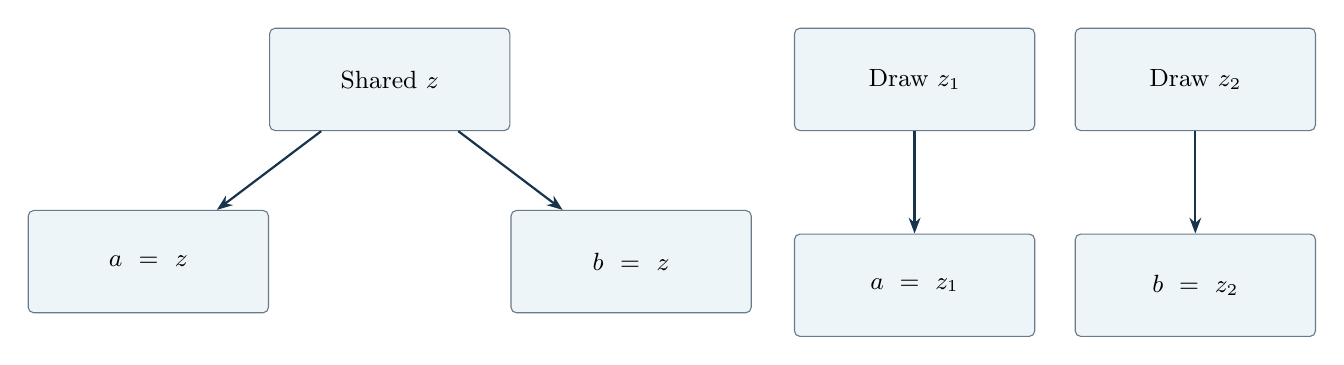
\begin{tikzpicture}
  \node[smallbox] (z) {Shared $z$};
  \node[smallbox,below left=10mm and 0mm of z] (a) {$a=z$};
  \node[smallbox,below right=10mm and 0mm of z] (b) {$b=z$};
  \draw[arr] (z) -- (a); \draw[arr] (z) -- (b);
  \node[smallbox,right=36mm of z] (u) {Draw $z_1$};
  \node[smallbox,right=5mm of u] (v) {Draw $z_2$};
  \node[smallbox,below=13mm of u] (c) {$a=z_1$};
  \node[smallbox,below=13mm of v] (d) {$b=z_2$};
  \draw[arr] (u) -- (c); \draw[arr] (v) -- (d);
\end{tikzpicture}
\end{center}

\subsection*{Two semantic routes remain open}
An operational route places measures over encoded closures and retained
machine states, with application specified by the evaluator. A denotational
route supports function spaces directly. Ordinary measurable spaces are
insufficient for the desired general higher-order structure; quasi-Borel
spaces provide a compositional alternative~\cite{QBS}, with domain-theoretic
extensions for recursion and recursive types~\cite{ProbDomains}.
Neither route should be confused with the existing mixture-of-kernels or
probabilistic-HOL-model modules, which do not implement a general probabilistic
lambda calculus. The small example above is a mathematical discriminator,
not a newly proved machine instance.

\sources{\name{Mettapedia/ProbabilityTheory/HigherOrderProbability/Basic.lean},
\name{Mettapedia/ProbabilityTheory/HigherOrderProbability/GiryMonad.lean},
\name{Mettapedia/ProbabilityTheory/IndependentFiniteSampling.lean}.}

\newpage
\subsection{Zooming requires a law for future computation}
\label{sec:zoom}

Let $v:S\to C$ forget details of a fine state. Equal coarse readouts now
are insufficient: different hidden states can react differently to the next
command. An exact coarse machine needs a law relating its future transitions
to those of the fine machine, for the declared action and observer family.

\begin{center}
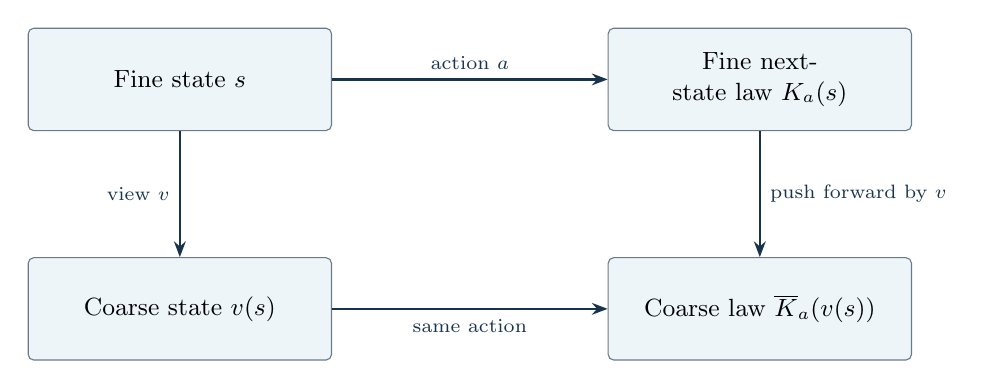
\begin{tikzpicture}
  \node[box] (s) {Fine state $s$};
  \node[box,right=35mm of s] (next) {Fine next-state law $K_a(s)$};
  \node[box,below=16mm of s] (coarse) {Coarse state $v(s)$};
  \node[box,below=16mm of next] (coarsenext) {Coarse law $\overline K_a(v(s))$};
  \draw[arr] (s) -- node[hint,above]{action $a$} (next);
  \draw[arr] (s) -- node[hint,left]{view $v$} (coarse);
  \draw[arr] (next) -- node[hint,right]{push forward by $v$} (coarsenext);
  \draw[arr] (coarse) -- node[hint,below]{same action} (coarsenext);
\end{tikzpicture}
\end{center}

For finite probabilistic states, existing strong lumpability says that states
in one view fibre have the same aggregated next-state law for every admitted
action. It constructs a representative-independent coarse kernel and proves
\[
 v_*\bigl(\mu\mathbin{\mathrm{bind}}K_a\bigr)
   =(v_*\mu)\mathbin{\mathrm{bind}}\overline K_a.
\]
Here $v_*$ is pushforward. Without this condition, retain additional state or
history, restrict actions/observers, or accept a weaker approximate contract.
A policy depending on hidden details also needs its own factorization law.

Existing probabilistic-square results offer a finite controlled-chain route
to approximation: local couplings bound expected discrepancy, and Lipschitz
and discount hypotheses control its accumulated observational effect.
They are not exact quotients or reversible maps. Numerical closeness also
depends on the observer: a finite floating-point distribution and a continuous
law can be maximally different in total variation despite close numerical
samples. A metric suited to the permitted queries may be more appropriate.

Zooming in can expose retained fine state or reconstruct an authorized view.
It cannot recover arbitrary forgotten choices from a non-injective quotient.
For the shared-draw example, the first call's marginal hides the captured
draw and whether subsequent calls reuse it; reconstructing by resampling
can break those correlations. Similarly,
replaying a native trace must not repeat committed effects. Observation,
demand and retention therefore remain separate in-language controls.

\subsection*{The remaining research question}
The missing joint theory is typed open-metagraph filling with scope, shared
identity, effects, probability and ownership, together with observation maps
that commute with continuation. Useful research would compare existing
models, identify incompatibilities, and work one higher-order shared/fresh
example through both exact finite execution and a continuous denotation.
General recursion, conditioning and scheduling must keep their explicit
conditions; universal complete inference is not a consequence of a universal
machine.

\sources{\name{Mettapedia/ProbabilityTheory/FiniteLumpability.lean},
\name{Mettapedia/Cybernetics/ApproximateAdequacy/ProbabilisticSquares.lean},
\name{Mettapedia/GSLT/Dynamics/ObservationSchedulerSufficiency.lean},
\name{Mettapedia/GSLT/Dynamics/ScheduleObservationFactorization.lean}.}

\newpage
\section{Qualification and the remaining joins}

An earlier shared resumption package extended eight existing semantic modules
without adding a Lean module. Its clean canonical build completed 5,547 jobs;
27 strict package/consumer checks and the declaration audit passed. The audit
covers 2,528 declarations, including 1,109 theorems, using only
\name{propext}, \name{Classical.choice} and \name{Quot.sound}.
The 1,058 GSLT controls produced identical output on CeTTa's PeTTa dialect,
the shared PeTTa checkout and the existing empty-superpose fork.

The earlier value-graph CAM, owned host with the retained rho chronicle, fixed C
core, its Cesta reader and its services were qualified together: the C11 and HE
language hubs build in 9,372 jobs, and the principal theorems and controls of these
packages use only the same three axioms. Their controls run Cesta-parsed C programs
to the values GCC and Clang compute, and serve C requests by the HE evaluator.

The joined resolver and machine migration has passed a serial strict check of
288 affected modules, including the recursive C-to-MeTTa service controls and
the translated MM0 and HOL consumers. An earlier 98-module receipt qualifies
the corresponding intermediate source state.
The HE oracle gate passes all 33 fixtures; the two-realization native gate
passes all 258 controls. The latter compares occurrence multisets across
realizations and retains each execution's own history. A subsequent complete
GSLT runner gate passes 1,230 named controls in 34 families, with identical
outputs on CeTTa and PeTTa, including the retained COMM controls. These runtime
checks do not establish source/native correspondence for arbitrary programs.

The query layer now proves that successful variable resolution is unique
across fuel and visited sets. In a binding record admitted by the native loop
filter, every successful recursive read agrees with public instantiation,
and the selected non-variable class value satisfies its instantiation equation.
That selected-value theorem is deliberately distinct from satisfaction of
every stored constraint: a raw record can contain another, inconsistent value
in the same class. The matcher now constructs the required consistency
invariant through its actual insertions, reconciliation and merges. On
float-free inputs its native instantiation satisfies every stored constraint;
successful native matches consequently pass the full independent dependency
criterion. The reverse matcher correspondence and its direct consumers have
been checked with that constructed invariant.

A structural change of binding layout is distinct from erasing execution
occurrences. Permuting the assignment and equality lists preserves all
class-dependency edges, semantic acyclicity and the executable cycle
decision. The lower equality-graph theorem requires only equal edge
membership; it does not identify the classes' enumeration order. Conversely,
adding an equality may create a cycle: the open assignment $x=f(y)$ becomes
cyclic after $x=y$. Recursive correspondence therefore retains both the
worker's exact record and the independent source record, related at their
declared representation boundary.

Representative order admits a more precise law than graph invariance.
Appending an already-stored equality preserves the first-appearance order,
every ordered class, its selected residual variable and its ordered direct
values. The extra native relation occurrence is retained. By contrast,
permuting two edges with the same membership can change the representative
from $a$ to $c$. Removing such a repeated logical edge preserves these observations;
arbitrary edge permutation does not justify that stronger conclusion.

A stronger record-permutation contract fails even on coherent alias frames.
Take assignments $x\mapsto F(z)$, $y\mapsto F(w)$, $z\mapsto A$,
$w\mapsto A$ with equality edges $(x,y)$ and $(z,w)$, then merge a fresh
private assignment to $B$. The actual HE-model reconciliation duplicates
the edge $(z,w)$; the independent singleton source merge preserves the
two-edge list. A checked inversion proves that no source endpoint is a
permutation of the three-edge result. Both endpoints nevertheless have the
same complete solution theory and the same tested joint readout, including
two uses of one open residual variable. This is a counterexample to the
representation contract, not an observable Rust or CeTTa defect.

The replacement must retain the concrete worker record for resumption and
compare its public observations through one coherent semantic readback.
Separate alpha witnesses for each value would not suffice: they could
forget whether two results share one residual variable. The existing
presentation-principality laws now connect to the executable HE binding
model's actual equality-aware resolver. Ordered class selection and the
unresolvable-value shortcut are checked against the canonical valuation;
the executable structural coverage bound supplies sufficient read depth.
Coherent acyclic records consequently yield one residual renaming for the
whole observation tuple, including repeated variables and private-frame
extensions. This is a theorem about the executable binding model, with
the actual C materializer correspondence still separate.

Joint alpha comparison alone does not license replaying a continuation under
the same commitments. An arbitrary extension of the observed variable map may
move an unobserved constrained name. For full solution-theory equality, the
comparison now has a stronger constructed form: one residual permutation
aligns the entire observed tuple, fixes every source model valuation pointwise,
and fixes every name outside the two observed residual supports. It therefore
preserves the complete source binding theory. The finite extension is made
inside fibres of the model-observation map, rather than choosing an arbitrary
permutation of names. Scoped observational equivalence alone does not supply
this stronger conclusion: a private equality may be visible only in one of
the two full theories.

The independent source endpoint need not itself be a coherent input to that
resolver. Its ordered equation fold constructs a normal exact finite
presentation. Mutual factorization of this presentation and the actual
principal readout yields one residual permutation for the complete observed
tuple. Thus source materialization is constructed even when directly running
the executable resolver on the source record would give an incorrect
principal observation. Repeated public and residual variables are compared
together, rather than by unrelated per-value alpha witnesses.

The chronological presentation is an additional representation convention,
not a consequence of the published binding theory. For the single equality
$\mathsf{public}=\mathsf{private}$, the current equation fold eliminates
$\mathsf{public}$, while the executable binding resolver retains it as the
class representative. A checked counterexample therefore refutes literal
equality between those two materializers, even at sufficient depth. The
independent query judgment now follows the published candidate-first merge
order. A constructed reversed-merge theorem transports the existing query
witness without changing its native binding record: both independent
endpoints have exactly the same full solution theory, although their row
layouts need not agree. Neither result licenses erasing variable spellings
from observable text.

That convention is nevertheless functional on fixed ordered rows.
Simultaneous induction through the three presentation-matching judgments
proves uniqueness of their output substitution; induction through the
equation fold then proves uniqueness of the complete presentation.
Every satisfiable record consequently has one joint historical readout for
all operands. This does not make it invariant under row permutation:
the equation lists $[(a,b),(a,c)]$ and $[(a,c),(a,b)]$ have the same complete
solution theory, but the fold reads $(a,a)$ as $(c,c)$ and $(b,b)$ respectively.
Both the positive folds and rejection of the opposite literal result are
kernel checked.

The mismatch is reached by an actual open query from an empty caller.
For the rule \code{(= (share \$x) \$x)}, the maintained query and merge
produce an alias between the public argument and a fresh rule variable.
The native-model request retains the public representative; the historical
source fold cannot emit it. Thus restricting the old equation-body contract
to reached caller records would still not repair that contract's hardwired
materializer. This is a counterexample to that source-model interface,
rather than a failure of the successful query.

The readback comparison also has a uniform executable form. Resolve the
complete finite binding support once and retain the nonidentity results as
a finite substitution. This one table agrees with every atom at sufficient
resolver depth, is normal and presents exactly the source solution theory.
It is not selected separately for each operand. A model-fixed residual
permutation relates it to the independent chronological presentation. This
constructs a finite representation of the executable HE binding model; it
does not establish the corresponding C decoder, nor determine a source
profile's history-sensitive representative policy.

The existing evaluator now carries this choice in one retained
\name{BindingFrame}. Its raw constraints are accompanied either by the
historical readout or by a finite table with a \name{ReadoutCertificate}.
The certificate relates that table to an independent equation fold through a
model-fixed residual permutation and certifies agreement for every future
operand. Renaming transports the constraints, the table and the certificate
together. It does not rename a previously produced string.

The current logical store now constructs such a presentation from its own
contents. Complete row enumeration retains each slot's generation, write
metadata and unbound status. Stored values carry their lexical context;
qualification names a variable by its full logical reference, so equal source
spellings in different frames remain distinct. The scoped preparation entry
checks every stored payload and the entire operand tuple against the actual
frame inventories and one explicit global-name context. An undeclared name
cannot silently become a shared global.

For unique acyclic assignments, the existing dependency-cycle decision
constructs a decreasing natural-number rank through the finite dependency
scheduler. The existing substitution fold then constructs the normal table
and its independent equation-presentation certificate. Admission requires no
supplied variable ordering. Every live operand uses that same table. Repeated
uses remain correlated, known unbound slots remain open, and stale contextual
references are refused. The scheduling witness establishes admissibility;
it does not select a common observable representative policy for all dialects.

An actual write into an open logical slot preserves the complete frame
inventory and adds exactly its new binding equation. Scope-checked preparation
and the two actual cycle checks reconstruct the updated certificate.
The stronger solution theory absorbs the old table for the entire pending
tuple, earning selected-frame renewal. An overwrite need not strengthen that
theory, and a scoped cyclic write can remain a valid storage operation while
falling outside this finite-tree readout admission. These results concern
one shared-store lineage. Rational values, correspondence with a language's
unification operation and physical implementation are separate obligations.

The normalized view also supplies a constructed immediate-function instance.
After an actual open-slot write and successful preparation, the existing
worker loads that view and the independent source step uses its certified
selected frame. Both reach the same invocation result through the actual
call and return transitions. The laws retain arbitrary caller and older
continuation data, a prior publication prefix and exact saved resumption.
They do not identify the raw store snapshot with a literal worker binding
record: loading the normalized view is an explicit representation step.

This is one mutually recursive evaluator, not a second selected evaluator.
All twelve judgment families carry the same frame. Pure transitions preserve
it literally; an actual query, merge or cast may renew its readout alongside
that operation's independent premise. A retained activation cannot silently
reselect a different valid table. Historical-mode preservation is proved
through the complete rule block. Existing function, raw-call, typed-return
and generated-dispatch consumers have been adapted through the complete
frame and explicit historical projections.

The source-execution relation additionally requires agreement with the actual
native-model table on every operand. An open query from an empty caller now
constructs the selected next frame from its physical source occurrence. The
controls follow two uses of one residual variable through a later real
unification and function return, obtaining \code{Pair A A}. They also reject
unlicensed table reselection, retain opaque rendered strings, and distinguish
an unfinished open call from its checked completion. These results concern
the maintained binding/control machine. A selected source derivation that
chooses another representative is not thereby proved to reflect into Rust
or C execution. Raw opaque binding payloads remain restricted to historical
frames until their actual saved representation carries the selected table.

Binding refinement supplies a separate compositional law. If a later frame
has a stronger complete solution theory, its normal finite presentation
absorbs the earlier presentation on every syntactic operand. The same law
holds for an ordered tuple of pending operands, preserving repeated uses and
shared variables. Actual successful match/merge and independent evaluator
extension laws now supply the required refinement; the published type
service earns its extension laws from its own matching and candidate scan.
Covered resolver calls may use different sufficient depths before and
after refinement. Rendered strings remain opaque: this absorption theorem
does not identify evaluation of an earlier string with rendering a later
representative.

The necessary coherence is also constructed by actual merge replay.
Starting with a unique, equality-free seed, each value conflict and class
join preserves pairwise agreement at a fixed canonical dependency
frontier. Recursive unifiers are confined to strictly smaller dependencies;
their replay establishes the pivot equations needed at the joined class.
Induction on the final dependency order then supplies canonical coherence.
For non-variable input assignments and a common finite-term model, the
actual solution-intersection law earns output loop freedom as well.
Thus a successful merge from an actual open match yields a principal
executable readout without assuming caller coherence or output
correspondence. Independent match and merge completeness then construct the
candidate-first source endpoint, its entire solution theory and its exact
freshness support. These are primitive query-boundary results; transporting
an arbitrary open continuation remains a separate obligation. Duplicate
native relation rows remain present throughout.

The independent unify and equation-query judgments now use
\name{LogicalMergeRel}: a successful merge has exactly the conjunction of the
two input constraint theories, exactly their union of support names, and a
finite model. This contract prescribes no relation-list layout or residual
representative. A concrete readout is a separate retained datum. Raw merge
replay supplies compatibility evidence when its output has an earned model;
neither an arbitrary raw merge nor its structural loop filter alone proves
consistency. A pure conservative-signature theorem transports native solution
implication to the larger structural atom signature, preserving the existing
model observations without importing an evaluator into the source rules.

The constructed operation \name{QueryBindingProjection.AliasReadout}
handles bare aliases in the incoming record. It exposes those assignments
as equality constraints before actual reconciliation and retains the structural
cycle filter. Each surviving occurrence earns the exact conjunction of the
original input theories, unchanged name support, a finite model and one
certified readout table. That table absorbs the old selected table across the
whole pending tuple. The result list is literally unchanged on callers whose
assignments contain no bare variables, including its order, multiplicity and
residual spelling. A crossed-alias control succeeds with all five observed
positions shared; structural occurs checks, rigid disagreement and inconsistent
seeds still refuse. The maintained recursive worker now uses this operation
at primitive unification and equation-query reconciliation boundaries; its
coverage checks and task denotation use the same boundary. The general raw
merge algorithm is unchanged. Stability after covered discovery does not
establish general source discovery completeness or justify treating budget
exhaustion as refusal.

Scoped comparison has explicit composition laws. Complete solution-theory
equality composes with the same added constraints; a scoped comparison
requires those new constraints' entire support to lie in its observation
scope. The negative controls distinguish these obligations. A tautological
equality changes freshness support while preserving every solution, and
adding a constraint on a hidden name can destroy scoped equivalence.
Hygiene support therefore remains a separate contract, rather than being
inferred from semantic redundancy.

The existing substitution algebra now also proves a support-determination
law. Two first-order substitutions produce the same pattern exactly when
their materialized variable values agree on that pattern's variable
occurrences. Consequently, they give the same template whenever its variables
are covered by the pattern. The source type-valuation interface is proved to
realize that same operation. An unused environment entry may differ;
an uncovered template variable need not agree. These laws concern structural
substitution and do not assume a quotient by object-language equations.

The ordinary recursive source family now constructs worker paths through
equation bodies, arguments and retained caller stacks. One uniform grammar
supports both relation-list permutation and complete solution-theory plus
hygiene-support comparison. The latter retains an independently certified
source readout table and agreement with every covered native-model read.
Principal native frames construct sufficient instances of this relation;
they are not required of every related frame. Its completion, encoded
execution, resumption, collection and
service-handler laws preserve each exact worker occurrence. Nested calls, a recursive
\code{peel} definition and duplicate physical equation declarations are checked.
The query-admission constructor now covers arbitrary finite closed first-order
patterns, including several and repeated variables, with a covered body
vocabulary. It constructs the match, merge, model, loop-freedom and body
materialization evidence from the actual hygienic query hit. The semantic
comparison admits alias-bearing reached callers and constructs the next
principal frame by reconciliation. A nested-call control retains three then
four equality occurrences while the corresponding independent source layout
differs. Completion, a reached pause, service delivery and one joint residual
observation are checked together. This remains a closed-query,
pattern-covered literal-result theorem. Open-query continuation transport,
general polymorphic/host cases remain outside that family's automatic
construction.

Typed invocation has a further constructed composition boundary. Declared
singleton arrows earn actual first-success selection and matcher coverage
from argument-domain evidence. The resulting head and argument paths compose
with an admitted minimal function body and its actual typed-return children,
preserving every ordered occurrence and the reached binding frame. The
raw-domain \code{function} annotation supplies a concrete instance: its body
syntax remains held until invocation, then a binding-changing body returns
two correlated uses through the ordinary receiver. A reached checkpoint
retains the nonempty bindings, caller and pending syntax and resumes exactly.
These constructions inhabit the existing recursive application judgment.
A nested duplicate-equation control follows ordinary return demand into a
typed function that changes bindings; its saved checkpoint retains both
receivers and the second source occurrence. Resumption preserves both results,
their separate reached bindings and an arbitrary older stack and output prefix.
This is admitted local source preservation and checked worker execution;
unrestricted source reflection, general polymorphic selection and physical
backend correspondence remain separate obligations.

The independent source evaluator has a simultaneous renaming action on all
twelve evaluator, return and minimal-control judgments. It transports the
whole space, live scope, saved caller, binding record and returned occurrences.
Its inverse reflects derivations, including the public success-priority rule.
The published type service is proved invariant by constructing lookup, casts,
argument applicability and the complete ordered candidate scan; arbitrary
foreign services remain explicitly transported components. This action does
not establish unchanged-default native adequacy.

Diagnostic rendering makes that distinction observable. A malformed minimal
\code{unify} embeds its rendered source atom, including fresh variable names,
inside a message symbol. Renaming variable leaves does not rewrite characters
already stored in that symbol. A checked source counterexample refutes
unchanged-renderer equivariance, whereas the named transported renderer admits
the renamed derivation. The following context also distinguished an actual
CeTTa compatibility defect from Rust HE:
\begin{verbatim}
(= (malformed)
   (function (chain (unify $a A B) $r (return $r))))
!(case (malformed)
   (((Error $s IncorrectNumberOfArguments) code) ($other text)))
\end{verbatim}
Rust returns \code{text}; the former compatibility boundary returned
\code{code}. The repaired boundary returns \code{text} and retains the source
subject. Successful four-argument calls and the other declared profiles retain
their behavior. This is a contextual branch, so treating diagnostic text as
non-normative would not establish contextual equivalence. The native formatter's
finite buffer remains a separate implementation limit.

There is also a fixed contextual separation, rather than only different
printed replies. Change one private rule variable from \code{\$a} to
\code{\$z}, keeping the public rule name and the entire observer unchanged.
The observer catches the message, formats it as a string, sorts it against a
fixed marker ending at the diagnostic prefix followed by \code{\$m}, and
tests whether that marker is first. Rust HE and both CeTTa execution paths
return \code{False} for the first program and \code{True} for the second.
Two activations of either program retain its respective Boolean. Ordering is
decided at the private letter, before the fresh numeric suffix; no generated
identifier is guessed. Well-formed primitive controls return the same
non-error token. Thus unrestricted contextual alpha-invariance is false for
this full observer language, even though the structural error subjects are
alpha-equivalent. A representation-independent profile must specify its
diagnostic and reflection policy; the binding-theory comparison alone cannot
establish that policy.

The distinction persists without an error. Consider this successful minimal
unification and its raw formatting result:
\begin{verbatim}
(= (probe)
   (function
     (chain (unify $a $z (format-args "{}" ($a)) Fail) $selected
       (chain (eval $selected) $text (return $text)))))
\end{verbatim}
Rust HE retains the left variable's spelling; the earlier CeTTa image
retained the right variable's spelling. Sorting the returned string against
the fixed marker \code{"\$m"} converts this difference to opposite ground
Booleans, before either numeric suffix matters. Swapping the two operands
reverses both results. These are equal first-order solution theories with
different observations in an unchanged context. The repaired HE-compat
primitive now retains the left representative after a successful match of
two distinct variables. Bound caller values, conflicts, both execution
paths and the previous raw-case protocol pass the independent runtime
controls; the other profiles retain their declared behavior. This narrow
repair does not reverse every matcher call:
other profiles deliberately orient their matches, and external matching
services may be asymmetric. The required comparison must retain each
profile's actual representative and materialization policy.

Fresh identity display is a separate observable boundary. A reflexive
\code{unify \$a \$a} keeps the same representative letter in both engines,
yet formatting exposes different generated suffixes. A fixed lexical marker
turns that difference into opposite ground Booleans on the pinned activation.
Unlike the letter-based control, this witness depends on that activation's
fresh supply. Correcting alias orientation alone therefore cannot establish
unrestricted equivalence for literal variable formatting; the freshness and
rendering policy must also belong to the declared profile.

A query can expose this choice without comparing different implementations
or changing the program. On the pinned Rust HE implementation, the following
closed program returns either ground Boolean on different executions:
\begin{verbatim}
(Pair $v $v)
!(let $text (match &self (Pair $a $z) (format-args "{}" ($a)))
   (let $sorted (sort-strings ($text "$m"))
     (== (car-atom $sorted) "$m")))
\end{verbatim}
Thirty-two fresh runs produced fifteen \code{False} and seventeen
\code{True} observations; repeated queries also varied within one process.
The bound-value control always returned \code{True}, and a query imposing
conflicting rigid values always returned the empty bag. The relevant source
route is \code{GroundingSpace::single_query}: it collects query variables in
a \code{HashSet}, then calls \code{narrow_vars}. The latter copies query
variables first and dependency variables second, choosing the first copied
member as each retained class's representative. One enumeration is shared
across the query's physical hits; it is not a separate choice for each
occurrence in a returned term. Both tested CeTTa execution paths instead
retained the stored variable's spelling and returned \code{True}.
These observations expose a representation choice through ordinary string
operations. They do not establish that HE promises deterministic spelling.
They do rule out deriving unrestricted contextual conformance solely from
equal binding solution theories: the adapter must justify the actual
narrowing and rendering policies as well.

A further compatibility control exposed a missing root-invocation route:
ordinary \code{case A ((A Hit))} returns \code{Hit}, while invoking that same
form through minimal \code{eval} returned \code{NotReducible} on the earlier
CeTTa image. Rust HE returns \code{Hit} through both routes. Its standard
library defines \code{case} by a minimal function body: it evaluates the
scrutinee and selects a branch. Arithmetic calls and ordinary effect calls
remain raw. Its \code{switch-minimal} protocol nevertheless enters a selected
\code{function} delimiter and converts selected \code{NotReducible} to
\code{Empty}; a bare \code{return} or \code{chain} remains syntax. A function
returning a print call yields that call without printing it. Thus neither
blanket holding nor blanket evaluation describes this boundary. The native
ordinary-case implementation alone does not supply this reflected root
invocation. Replacing the missing route by complete branch evaluation would
also be incorrect when the selected branch contains effects. The repaired
HE-compatibility route reuses the existing scrutinee capture and first-match
builder, publishes the substituted template with its actual bindings, and
leaves function entry to the existing raw-return continuation. Native controls
retain duplicate scrutinee occurrences, select only the first matching clause,
distinguish a missed clause from an empty scrutinee, and check the raw effect
boundary. An independent comparison against Rust passes on both native
execution paths with bounded and unbounded scheduling and collection enabled;
the earlier image remains a negative control. Other profiles retain their
declared behavior. This is a qualified native repair, not a whole-interpreter
source correspondence theorem.

Minimal invocation must also expose the standard library's actual one-step
program. In Rust HE,
\texttt{eval (let \$a 7 \$a)} returns
\texttt{(unify 7 \$a \$a Empty)}, rather than the final value $7$.
The caller's continuation and demand decide whether that program subsequently
runs. The compatibility implementation now installs the actual library
equation on its imported-library boundary. Querying that equation, raw
invocation and full evaluation consequently use the same stored occurrence;
repeated user equations retain their separate alternatives. An intrinsic
that merely synthesizes the same final value would not establish this
source-observation property.

A second native repair composes minimal function completion with the
caller's typed result continuation. A named untyped function that returns
\code{(println! 9)} prints once; a bare function with the declared
\code{Atom} return demand keeps that expression as data. A named function
whose body is \code{(println! 9)} without a return marker instead yields
\code{NoReturn} and does not print. Independent replay of a named
\code{chain}/\code{let}/\code{eval} example now returns $7$ on Rust HE and
both native execution paths. A subsequent compatibility query repair
publishes a terminal variable under its unique projected query representative
and rewrites the carried bindings consistently. It does not choose a name when
two query variables share that terminal. The six earlier letter-representative
failures are closed in the recorded 96-cell correlation gate. Generated private
suffixes and multiply represented classes retain their separate observable
boundaries; this is not unrestricted literal-name conformance.

A nonempty returning-function example exposed an additional native crossing:
\begin{verbatim}
(= (wrap $x $y) (function (return (got $x $y $x $y))))
!(let ($r) (collapse (wrap $a $a)) (== $r (got $a $a $a $a)))
\end{verbatim}
Before the repair, canonical native execution returns \code{True}, while the
noncanonical delimiter returns \code{False}: its collected value contains the
private terminal of the rule-variable chain. Both paths now use the same
compatibility-profile query-representative operation. The canonical
\code{CALLER} frame already applies its reached environment; that application
has not been replaced by a synthesized answer. The repaired image passes 80
maintained fixture executions and 20 independently replayed focused controls,
including the earlier failing image. Its retained-execution gate checks a
returned effect with a bound argument at 52 pause points, with cancellation,
and commits the effect once. Extended and formal profiles retain their own
readout policies. These executions do not supply the still-missing general
physical proof for nonempty binding application and \code{CALLER}; the Rust
representative boundary below also remains explicit.

The same investigation exposed an independent source-model defect:
\begin{verbatim}
(= (foo) (function (SomeValue)))
!(eval (foo))
\end{verbatim}
Both Rust HE and the two native execution paths return
\code{(Error (foo) NoReturn)}. The former source rules admitted
\code{(Error (SomeValue) NoReturn)} because equation and host invocation
completion omitted the saved call. The four raw/typed equation/host rules
now supply the assembled invocation as the nearest caller. Embedded minimal
instructions retain their ambient continuation. Generic exact laws for
closed data bodies cover both historical and retained finite readouts; a
negative control rules out the old body-origin answer at this completion
boundary. The correction uses the existing judgments, rather than a second
evaluator. Two maintained Rust fixtures exercise raw and full evaluation.

A second source-model defect concerned the boundary between ordinary and
minimal invocation. The actual annotated call
\code{(function (return 7))} returns $7$ on Rust HE and both native paths,
whereas the former full source judgment admitted its unchanged wrapper.
Its equation fallback had not excluded embedded instructions. An ordinary
\code{unify} could also publish its selected template without passing the
ordinary typed return gate. With \code{(= (f) Value)}, ordinary
\code{(unify X X (f) Fail)} returns \code{Value}, while the explicit raw
\code{eval} form returns \code{(f)}. The repaired source judgment delegates
embedded invocation to the existing minimal relation and then to the existing
ordinary return relation. Their exact composition law retains the reached
binding frame and selected demand; it preserves the separate producer-completed
native lane. Malformed-unify diagnostics now belong to the primitive step and
retain their declared renderer. A negative control excludes the unchanged
function wrapper and another excludes erasing a selected binding readout.
Successful primitive selection also has to read its template through the
selected frame. With \code{(= (f A) Hit)}, the program
\code{(unify \$x B (f \$x) Fail)} returns \code{(f B)}. Constraint evidence
alone would permit publishing the unread template; it does not determine the
emitted syntax. The repaired success rule requires the actual match/merge
candidate, frame renewal and exact materialization. Refusal instead retains
the identical complete frame and the raw fallback. Separate controls preserve
two uses of one variable, keep variable-looking string data opaque, and reject
discarding the retained readout. An exhausted equation query uses
\code{NotReducible}; the ordinary return gate restores its saved invocation.
This query fallback is distinct from a host operation's empty-result protocol.

The maintained corpus now passes 40 Rust cases, with all earlier bags
unchanged and source anchors checked. The frozen native compatibility image
also passes all 40 cases under both canonical execution settings: 80 executions,
with multiplicity preserved and no alpha normalization. The coherent eight-owner repair passes
strict compilation. Its audit covers 6,805 kernel declarations and 3,629
theorem declarations, using only the standard three Lean axioms; 16 generated
compiler implementations are validated separately. These are source-model
repairs and local adequacy results, not whole-interpreter correspondence.

The retained source admission now constructs minimal data, admitted
unification success and genuine no-match, cons/decons, recursive function
bodies and ordinary embedded calls in the existing mutual family. Successful
unification uses the actual match and merge to construct the selected next
frame. Each function-body result is read in its own reached frame before the
continuation resumes an instruction. Ordinary calls compose that minimal
execution with the independent typed-return judgment. Checked completion and
saved resumption preserve the same admission, original caller and prior output.
Controls retain two pending uses through a real binding change and an actual
four-step checkpoint. Completed producer provenance keeps function-looking
result data separate from emitted code.

Equation admission now composes the actual query occurrence, prepared input,
emitted producer execution and typed return. Function-producing equations run
their bodies through the same primitive and continuation machinery before
resuming the ordinary receiver. The three ordered occurrence coordinates
remain distinct; the previous nonfunction equation path is a proved
singleton-producer specialization. Checked completion determines the entire
delivered result list and publication prefix, and each occurrence has an
independently derived source call at its reached frame. Two identical physical
equations retain two results and distinct fresh bindings. An actual
thirteen-step checkpoint retains an active function, the second producer and
the ordinary receiver, then resumes exactly. Nine executions on Rust HE and
both native canonical settings agree on twelve ground observations, including
the original caller in a non-returning function error.

Raw invocation and structural \code{chain} now compose in this same mutual
admission family. Raw \code{eval} reads its actual input frame, runs the
selected equation's producer and returns through the raw receiver. A chain
reads each child's reached frame, substitutes its explicit destination into
the saved syntax, then resumes the existing minimal continuation under the
original caller and live scope. It does not install that structural destination
as a new binding assignment. The constructed completion, whole-result-list
uniqueness, per-occurrence source meaning and saved resumption laws apply to
these admitted requests. They do not assume a completed suffix or a whole-run
correspondence as local evidence.

Checked controls compose a raw query, two identical physical equations,
function-producing bodies, a two-use chain template and an enclosing function.
An actual twenty-step checkpoint retains seven continuation frames and both
fresh nonempty result bindings; resumption delivers both occurrences. A
binding-changing unification also reaches both pending uses correctly.
Separate controls distinguish genuine query absence, ordinary restoration,
internal \code{Empty} and depth suspension. Three Rust/native executions agree
on twelve ground observations. General non-symbol-headed raw invocation,
all-filtered queries, polymorphic applicability, embedded-head typing and
effectful host/world composition remain separate admission obligations.

The authored \code{switch-minimal} library has a separate boundary. Rust gives
it the type \code{(-> Atom Expression Atom)}; it is not an embedded primitive.
Ordinary invocation and raw invocation both hold the selected \code{(f)}
in the example above. The source model's unconditional switch shortcut has
been removed in favor of actual authored equations. The repaired frozen native
compatibility image now agrees with Rust on both entries; its seven boundary
programs pass in both native canonical execution settings. This closes the
concrete library-return discrepancy. The general retained invocation
correspondence remains a separate obligation.

An open-answer control exposes a stronger representative boundary than
printing. Consider
\begin{verbatim}
!(let ($r)
  (collapse (let (pair $x $y) (pair $a $b) (got $x $y)))
  (== $r (got $a $b)))
\end{verbatim}
In 24 fresh processes of the pinned Rust HE 0.2.10 executable, this program
returns \code{True} 13 times and \code{False} 11 times. The result is a ground
Boolean, so renaming printed result variables cannot explain the difference
away. The branch's equality-class representative is materialized into the
collapsed atom; its branch bindings are then absent from the outer comparison.
A native candidate consistently selects the earliest left-operand variable
and returns \code{True} under both execution settings. The unchanged corpus
and separate duplicate-occurrence controls pass, but this policy is not thereby
literal equivalence to all Rust observations. A proposed deterministic
readout contract must state what correlation with caller variables survives
collapse. Complete solution-theory preservation before projection does not
alone preserve later literal-equality observations after the binding context
has been discarded.

One actual full-evaluation behavior remains under investigation. Bare
\code{(function (println! 9))} prints nothing but returns an unresolved
\texttt{\$result\#17} on a fresh pinned Rust process; a preceding evaluation
changes its generated identity. The named non-returning form gives the
expected caller-origin error. Native compatibility instead retains the
minimal \code{NoReturn} result for the bare form. The unresolved internal
plan variable, the minimal error and the caller's full result are distinct
observations. A proposed semantic repair must identify that boundary and
state its profile explicitly; inventing a matching fresh-name counter would
not explain it.

An isolated SWI-PeTTa experiment illustrates the distinction between machine
refinement and a small semantic change. Direct \code{(/ 1 0)} and its
\code{eval} entry raise the host zero-divisor exception. Dynamic
\code{(reduce (/ 1 0))} catches every host exception and instead fails as a
Prolog goal, so subsequent top-level commands continue. Removing that catch
in one isolated process makes dynamic dispatch propagate the same exception;
an explicit MeTTa catch then receives the structured error. Ten program pairs
retain successful arithmetic, duplicate answers, ordinary failure, unknown
syntax and shared variables while exposing that deliberate fault-policy
change. The production translator is unchanged. This experiment proves neither
a general SWI compiler correspondence nor a speedup; it identifies a small
candidate whose semantic benefit can be assessed against actual programs.

The existing PeTTa source and streaming owners now carry a destination-aware
relational continuation alongside the eager policy. Destination matching may
reject a rigid data skeleton before evaluating its contents; a primitive
producer can instead commit its effect before its result fails to match the
destination. The local native goal-array square retains older requests,
bindings, world and occurrence positions. Its admitted structural region is
explicit: list cells, rational terms and specialized scalar routing require
their own readbacks. A suspended child reply is
distinct from a request for another child, and consumed rows cannot be replayed.

The finite store presentation now instantiates this destination return step.
Scope-checked preparation supplies the actual equations and one table for the
value, destination, result and older goals. The independent return judgment
accepts or refuses exactly when its materialized counterpart does. Successful
resolution constructs one residual-variable permutation for the entire live
tuple. Future solutions of the extended equations absorb the earlier table,
preserving repeated uses. The actual saved-cursor laws retain the world,
output, caller context and pending goal occurrences; resumption uses that
cursor rather than repeating the earlier print. Refusal completes the branch
with its reached world and differs from budget exhaustion. This instance
uses finite first-order constraints within the declared acyclic store
profile. Its event carrier is empty: the retained-world result is not a
physical C receipt theorem. Choice, collection and additional primitive or
equation invocation policies need their remaining operational joins.

Argument return has a separate local source judgment: its saved continuation
is a younger/older list split, represented by a checked finite delimiter.
A normal value continues the whole pending list. An error bypasses the younger
argument work and constrains the outer destination with the reached equations.
Refusal preserves the reached world; a malformed delimiter is a distinct
boundary. Actual argument scheduling preserves delimiter validity, as does
every exhausted prefix, so an admitted run cannot reach that malformed state
at any budget. The scope-checked current-store instance uses one table for
the returned value and every younger and older goal operand. The print step
commits its output before result matching, and arbitrary saved prefixes compose
with exact resumption. Other invocations retain their resolved arguments and
continuation as requests; retaining a request is not executing it.

Collection exposes a further source-model defect:
\begin{verbatim}
!(let ($a $b) (collapse (superpose ($x $x))) (== $a $b))
\end{verbatim}
SWI-PeTTa and the native PeTTa path both return \code{false}. Each collected
answer has its own fresh variables, while repeated uses within that answer
remain shared. The current eager logical collector instead reuses the same
variable across the two answers and returns \code{true}; a kernel-checked
computation establishes that disagreement. A maintained four-query reference
also retains duplicate ground answers, tests binding one answer before reading
the other, and distinguishes sharing within an answer from sharing between
answers. Both implementations pass all four observations. A faithful
collection rule must copy an answer and its associated retained syntax with
one renaming, independently of other answer copies. Renaming printed output
cannot repair the ground Boolean disagreement.

The retained terminal-copy component is now constructed in the existing scope
carrier. An actual completed destination run determines its terminal prefix;
the collector reads that reached cursor, appends its value, equations and
occurrence, then computes independent answer copies before installing the
saved caller. The laws retain the reached shared world, caller bindings and
context, older alternatives and prior answer metadata. One injective renaming
serves each answer and its associated syntax, with disjoint complete tuples
between answers. A kernel computation of two actual returns followed by the
existing equality operation gives \code{false}.

The existing retained driver now also has an explicit scoped destination
profile. Its finite loader jointly qualifies authored code, cells, operands
and caller context. The scheduler constructs child entry, follows actual
equation and primitive operations, copies completed answers, restores the
caller and retains the shared world. Empty search is distinguished from
refusing one branch; faults and associated work retain the exact saved scope.
Every finite prefix preserves scope nesting, and every published occurrence
has independently satisfiable reached constraints. Local mutable-operation
laws preserve the identity inventory from the actual supported payloads.
Controls execute nested collection, within-answer correlation, distinct answer
copies and effectful refusal with exact resumption. The old eager default
remains unchanged. Arbitrary dynamically created variable names, complete
provenance through future world updates and execution of associated work
remain further obligations; the profile is not a whole-language or physical
backend correspondence theorem.

Finite clause selection likewise executes the existing solver rather than
receiving a chosen solution. A shared freshening covers the pattern and body;
the independent common-solution judgment characterizes both acceptance and
refusal. Physical source occurrences, including identical equations, survive
selection. The current-store instance supplies one readout for all pending
operands and retains the selected body as work for the actual continuation.

Type-search paths and answer occurrences have different roles. The actual
Rust evaluator chooses the first successful pair in the flattened scan of
function types and their applicability bindings. For example,
\begin{verbatim}
(: ident (-> Atom Atom))
(: ident (-> Number Number))
(= (ident $x) $x)
!(collapse (ident 7))
\end{verbatim}
returns \code{(7)} in both the pinned Rust evaluator and native compatibility
settings. One arrow with two successful argument-type paths likewise produces
one answer. Repeating the defining equation instead produces \code{(7 7)}.
The older all-candidate Lean evaluator duplicates the first example; retaining
every successful binding from one callback also duplicates the second.
These controls identify model discrepancies. A faithful implementation must
honor the declared selection boundary while retaining subsequent equation
occurrences; backend scheduling freedom does not authorize extra answers.

Polymorphic instantiation exposes another source-model boundary:
\begin{verbatim}
(: ident (-> $t $t))
(= (ident $x) $x)
!(Pair (ident 7) (ident True))
\end{verbatim}
The pinned Rust and native compatibility executions return \code{Pair 7 True}.
The maintained retained worker currently rejects the second call because its
annotation lookup reuses the declaration's variable after the first call has
constrained it to \code{Number}. A call-site instance must freshen the whole
arrow against the complete saved configuration, preserving repeated domain
and return variables within that arrow while separating successive calls.
Raw declaration lookup remains useful for inspection. This is a model scope
defect, not evidence that either checked implementation rejects the program.

The first-success worker now also uses the common checked resource interface.
Its coverage predicate follows the failed applicability prefix and selected
candidate, then stops; an unselected divergent suffix creates no obligation.
Depth exhaustion retains a request and complete saved configuration. Genuine
empty completion is distinct. A completed checked execution gives the same
full result at every larger pending evaluator depth, with exact structured
and encoded resumption. The recursive controls construct the required checked
runs. Finite source evidence alone does not yet construct sufficient coverage
for every bounded matcher leaf. A stronger constructed route now adds local
coverage for precisely the reached type selections, casts, query, merge and
materialization leaves. Induction on that source derivation yields a finite
checked worker path and hence a sufficient scheduler budget, valid at every
larger budget. Every actual exhausted scheduler checkpoint resumes to the
same completed occurrences from its saved state. Closed type casts obtain
their local bound from syntax size; arbitrary open or foreign leaf coverage
remains an explicit further construction.

Variable support is also preserved through the actual native binding
operations. Every name returned by reconciliation or merge comes from an
input equation or binding record. Recursive resolution introduces no name
outside its input term and the complete caller record; projection introduces
no name outside that record, even if an unbound name was requested.
Freshness therefore includes dependencies inside open stored values.
A local may acquire equality aliases during matching while its class remains
valueless. Assigning a closed value to such a class retains the complete
caller, and the executable loop check still selects success or refusal.
The existing fresh-variable API is derived from this class-level law.

The shared binary argument fold also records each result's physical input
occurrence and the state reached after all earlier input occurrences. Its
origin theorem retains arbitrary incoming bindings and both actual
merge/projection boundaries. Equal first results can therefore lead to
different later effects without being merged: the controls execute the next
argument in successive states, while a changed terminal suppresses that
argument entirely. These are laws of the existing worker's chronology, not a
global MeTTa enumeration policy.

These are package-specific qualification results, not completion of every
machine or of the whole source/native goal. Separate historical receipts
qualify earlier CAM, VM and native-boundary packages. A full joined acceptance
must identify the exact current sources, assumptions, executable consumers
and relevant runtime gates.

\begin{tabularx}{\linewidth}{@{}p{34mm}X@{}}
\toprule
Package & Remaining constructed connection \\
\midrule
Common theory & Legal contextual closure and observer/scheduling joins for
the actual language instances. \\
MeTTa & Complete source/configuration/native correspondence at arbitrary
nesting, preserving raw/quoted boundaries, sharing, worlds, occurrences and
each worker's retained history. Live-scope equation lookup and checked
completion now support nested calls and recursive services; the complete
contextual correspondence remains open. LeaTTa-only coverage and conformance
are optional supporting results; they do not discharge the CeTTa connection
or block its acceptance. \\
Interaction & Complete contextual MeTTa/effectful interaction joins.
The retained rho runner now constructs both orders of disjoint COMMs,
with exact histories, dependency validation, cancellation and no replay.
Crash recovery and distributed agreement are separate host assumptions. \\
CAM & Joined current-source qualification. Extended scoped readback and
memoizing execution now have bidirectional correspondences with their
independent source judgments, including captured scope and nested demand. \\
Fixed C core & The common fixed/located fragment now covers successful and
faulting source histories, licensed expression/assignment refusals and exact
retained budget splits. Its whole-run reverse simulation discovers the owning
source controls from arbitrary licensed located histories, including partial
assignments and loops. Joined current-source qualification remains.
Named extensions such as \code{for}, \code{do}, \code{switch}, array
initializers and calls inside expressions remain outside the fixed core. \\
Joined acceptance & Full relevant runtime gates and current-source audits
through the shared interfaces. Recursive MeTTa services and retained logical
checkers have package-specific qualification; this does not supply the whole
source/native correspondence. \\
\bottomrule
\end{tabularx}

The priority is to close the complete MeTTa representation and owned
interaction joins. The productive block laws, actual retained searches and
world-query certificates already provide reusable pieces. Extending another
independent framework would not replace those connections.

\begin{thebibliography}{99}
\bibitem{CAM}
G. Cousineau, P.-L. Curien and M. Mauny.
\emph{The categorical abstract machine}.
Science of Computer Programming 8(2), 173--202, 1987.
\url{https://doi.org/10.1016/0167-6423(87)90020-7}.

\bibitem{AlgebraicStepper}
J. Clements, M. Flatt and M. Felleisen.
\emph{Modeling an Algebraic Stepper}.
ESOP 2001, Lecture Notes in Computer Science 2028, 320--334.
\url{https://doi.org/10.1007/3-540-45309-1_21}.

\bibitem{LetRewriting}
F. J. L\'opez-Fraguas, E. Martin-Martin, J. Rodr\'iguez-Hortal\'a and J. S\'anchez-Hern\'andez.
\emph{Rewriting and narrowing for constructor systems with call-time choice semantics}.
Author manuscript, 2012.
\url{https://arxiv.org/abs/1209.2617}.

\bibitem{Refocusing}
O. Danvy and L. R. Nielsen.
\emph{Refocusing in Reduction Semantics}.
BRICS Report RS-04-26, 2004.
\url{https://www.brics.dk/RS/04/26/BRICS-RS-04-26.pdf}.

\bibitem{ITrees}
L. Xia, Y. Zakowski, P. He, C.-K. Hur, G. Malecha, B. C. Pierce and S. Zdancewic.
\emph{Interaction Trees: Representing Recursive and Impure Programs in Coq}.
Proceedings of the ACM on Programming Languages 4, POPL, Article 51, 2020.
\url{https://doi.org/10.1145/3371119}.

\bibitem{ZINC}
X. Leroy. \emph{The ZINC Experiment: An Economical Implementation of the ML Language}.
INRIA technical report 117, 1990.
\url{https://xavierleroy.org/publi/ZINC.pdf}.

\bibitem{MultiLanguage}
J. Matthews and R. B. Findler.
\emph{Operational Semantics for Multi-Language Programs}.
ACM Transactions on Programming Languages and Systems 31(3), Article 12, 2009.
\url{https://doi.org/10.1145/1498926.1498930}.

\bibitem{ScopeSets}
M. Flatt. \emph{Binding as Sets of Scopes: Notes on a New Model of Macro
Expansion for Racket}.
\url{https://users.cs.utah.edu/~mflatt/scope-sets-2/}.

\bibitem{Derivative}
C. McBride. \emph{The Derivative of a Regular Type is its Type of One-Hole
Contexts}. Extended abstract, 2001.
\url{http://strictlypositive.org/diff.pdf}.

\bibitem{Zipper}
G. Huet. \emph{The Zipper}. Journal of Functional Programming 7(5),
549--554, 1997.
\url{https://www.cs.tufts.edu/comp/150FP/archive/gerard-huet/zipper.pdf}.

\bibitem{ProbNondet}
D. Varacca and G. Winskel. \emph{Distributing probability over
non-determinism}. Mathematical Structures in Computer Science 16(1),
87--113, 2006.
\url{https://www.cl.cam.ac.uk/~gw104/distprobnd_journal.pdf}.

\bibitem{ReflectiveMetagraph}
B. Goertzel. \emph{Reflective Metagraph Rewriting as a Foundation for an
AGI ``Language of Thought''}. arXiv:2112.08272.
\url{https://arxiv.org/abs/2112.08272}.

\bibitem{QBS}
C. Heunen, O. Kammar, S. Staton and H. Yang.
\emph{A Convenient Category for Higher-Order Probability Theory}.
LICS, 2017. \url{https://arxiv.org/abs/1701.02547}.

\bibitem{ProbDomains}
M. V\'ak\'ar, O. Kammar and S. Staton.
\emph{A Domain Theory for Statistical Probabilistic Programming}.
Proceedings of the ACM on Programming Languages 3, POPL, Article 36, 2019.
\url{https://arxiv.org/abs/1811.04196}.

\bibitem{RosettaStone}
J. C. Baez and M. Stay.
\emph{Physics, Topology, Logic and Computation: A Rosetta Stone}.
In B. Coecke (ed.), \emph{New Structures for Physics},
Lecture Notes in Physics 813, pp. 95--172, 2010.
\url{https://doi.org/10.1007/978-3-642-12821-9_2};
\url{https://arxiv.org/abs/0903.0340}.

\bibitem{RewritingLogic}
J. Meseguer. \emph{Conditional rewriting logic as a unified model of concurrency}.
Theoretical Computer Science 96(1), pp. 73--155, 1992.
\url{https://doi.org/10.1016/0304-3975(92)90182-F}.

\bibitem{SecondOrderMetatheory}
M. Fiore and D. Szamozvancev.
\emph{Formal Metatheory of Second-Order Abstract Syntax}.
Proceedings of the ACM on Programming Languages 6, POPL, 2022.
\url{https://doi.org/10.1145/3498715};
\url{https://arxiv.org/abs/2201.03504}.

\bibitem{MM0}
M. Carneiro. \emph{Metamath Zero: The Cartesian Theorem Prover}.
arXiv:1910.10703. \url{https://arxiv.org/abs/1910.10703}.

\bibitem{HOLLight}
J. Harrison. \emph{HOL Light: An Overview}.
\url{https://www.cl.cam.ac.uk/~jrh13/papers/hollight.html}.

\bibitem{Lean4Lean}
M. Carneiro. \emph{Lean4Lean: Verifying a Typechecker for Lean, in Lean}.
arXiv:2403.14064, version 3, 2025.
\url{https://arxiv.org/abs/2403.14064}.

\bibitem{Lean4Less}
R. Vaishnav. \emph{Lean4Less: Eliminating Definitional Equalities from Lean
via an Extensional-to-Intensional Translation}. ICTAC 2025.
\url{https://rish987.github.io/files/lean4less.pdf};
\url{https://github.com/Deducteam/Lean4Less}.

\bibitem{LambdapiRules}
Lambdapi contributors. \emph{Lambdapi User Manual: Commands, rewrite rules}.
\url{https://lambdapi.readthedocs.io/en/stable/commands.html}.

\bibitem{CakeMLProofMachines}
CakeML contributors. \emph{CakeML projects and verified applications}.
\url{https://www.cakeml.org/projects.html};
\url{https://cakeml.org/}.

\bibitem{OpenTheoryArticle}
J. Hurd. \emph{OpenTheory Article File Format}.
\url{https://www.gilith.com/opentheory/article.html}.

\bibitem{MathlibPartrecCode}
{\raggedright
Mathlib contributors. \emph{G\"odel numbering for partial recursive functions}.
\code{Mathlib.Computability.PartrecCode}, especially \code{exists\_code},
\code{evaln\_sound}, \code{evaln\_complete} and \code{primrec\_evaln}.
\url{https://leanprover-community.github.io/mathlib4_docs/Mathlib/Computability/PartrecCode.html}.\par}

\bibitem{DynamicStrategyPriority}
M. Rawson and G. Reger. \emph{Dynamic Strategy Priority:
Empower the strong and abandon the weak}. PAAR, 2018.
\url{https://rawsons.uk/michael/papers/PAAR-2018.pdf}.

\bibitem{LRAT}
L. Cruz-Filipe, M. J. H. Heule, W. A. Hunt Jr., M. Kaufmann and
P. Schneider-Kamp. \emph{Efficient Certified RAT Verification}. CADE, 2017.
\url{https://www.cs.cmu.edu/~mheule/publications/lrat.pdf}.

\bibitem{EkerAC}
S. Eker. \emph{Associative-Commutative Rewriting on Large Terms}. RTA, 2003.
\url{https://maude.cs.illinois.edu/papers/abstract/EkerACrewriting_2003.html}.

\bibitem{WellPointed}
J. Ad\'amek, S. Milius, L. S. Moss and L. Sousa.
\emph{Well-pointed coalgebras}. Logical Methods in Computer Science 9(3:2),
2013. \url{https://lmcs.episciences.org/704/pdf}.

\bibitem{TuriPlotkin}
D. Turi and G. Plotkin. \emph{Towards a Mathematical Operational Semantics}.
Proceedings of LICS, 1997, pp. 280--291.
\url{https://homepages.inf.ed.ac.uk/gdp/publications/Math_Op_Sem.pdf}.
\bibitem{WeinbaumThesis}
D. R. Weinbaum (Weaver). \emph{Open-Ended Intelligence}.
PhD thesis, Vrije Universiteit Brussel, 2018, especially Chapters 5 and 7.
\bibitem{nLabInference}
nLab contributors. \emph{Deductive system}, \emph{multicategory},
\emph{syntactic category}, and \emph{institution}.
\url{https://ncatlab.org/nlab/show/deductive+system};
\url{https://ncatlab.org/nlab/show/multicategory};
\url{https://ncatlab.org/nlab/show/syntactic+category};
\url{https://ncatlab.org/nlab/show/institution}.
\end{thebibliography}
\end{document}
